% ECE441 Lab 4 report. Compile with pdfLaTeX, XeLaTeX, or Tectonic.
% Keep the figures/ directory beside this file. The complete download includes it.
% Numbers and images are from the existing analysis; no new EEG analysis is claimed.
% Complete the author information below before submission.
\documentclass[11pt,a4paper]{article}
\usepackage[T1]{fontenc}
\usepackage{lmodern}
\usepackage[margin=22mm]{geometry}
\usepackage{microtype}
\usepackage{amsmath,amssymb}
\usepackage{graphicx}
\usepackage{float}
\usepackage{booktabs,tabularx}
\usepackage{caption}
\usepackage[section]{placeins}
\usepackage{enumitem}
\usepackage{xcolor}
\usepackage[hidelinks]{hyperref}

\graphicspath{{figures/}{../../report/img/}{report/img/}{img/}}
\captionsetup{font=small,labelfont=bf,skip=5pt}
\setlength{\parindent}{1.2em}
\setlength{\parskip}{3pt}
\setlength{\textfloatsep}{12pt plus 2pt minus 2pt}
\setlength{\floatsep}{10pt plus 2pt minus 2pt}
\setlength{\intextsep}{10pt plus 2pt minus 2pt}
\setlist{nosep,leftmargin=*}
\renewcommand{\arraystretch}{1.13}
\emergencystretch=1.5em
\newcommand{\uv}{\ensuremath{\mu\mathrm{V}}}
\newcommand{\ep}{\ensuremath{\hat p}}

\title{EEG responses to targets and non-targets\\in a visual oddball task}
\author{Laurence Yang (1010500520)\\[2pt]
  \small [Member 2 name and student number]\\
  \small [Member 3 name and student number]}
\date{ECE441, Lab 4}

\begin{document}
\maketitle
\vspace{-1em}

\section{Introduction}

We recorded EEG during a visual oddball task in which a participant pressed a
button for red circles and ignored blue squares. Each run contained 15 circles
and 75 squares. The task tests whether the responses to rare targets differ from
those to frequent non-targets. A common response in oddball tasks is the P300,
a late positive potential with a centro-parietal maximum \cite{polich}.

We compared the two conditions in two recordings from the same participant,
using the cluster-based permutation test of Maris and Oostenveld \cite{maris}.
The analysis follows the lab's single-channel procedure, with an additional
correction across the eight electrodes. We analysed the runs separately and
also combined their trials.

The analysis code is available at
\url{https://github.com/Echo078/ece441_lab4}.
The statistical functions are in \texttt{lab4\_stats.py} and the processing
pipeline is in \texttt{lab4\_analysis.py}; code screenshots are included in
Appendices~\ref{app:statscode} and~\ref{app:analysiscode}.

\section{Cluster-based permutation testing}

An epoch in the main analysis contains 176 time samples on each of eight
channels. Testing every sample separately at $\alpha=0.05$ creates a multiple
comparisons problem. Bonferroni correction controls the family-wise error rate,
but does not use the temporal structure of EEG. The cluster test uses that
structure by combining neighbouring samples into one statistic.

For each channel, we calculate a two-sample $t$-test at every time point.
Adjacent samples with two-sided $p<0.05$ form a cluster, with positive and
negative $t$-values grouped separately. The sum of the $t$-values is the cluster
mass. We retain the cluster with the largest absolute mass:
\begin{equation}
  T_c=\max_{K\in\mathcal{K}_c}\left|\sum_{t\in K}t_c(t)\right|,
\end{equation}
where $\mathcal{K}_c$ is the set of clusters on channel $c$. We set $T_c=0$
when no cluster is present and retain the selected cluster's sign when
reporting its mass.

Under the null hypothesis, trials from the two conditions are exchangeable.
Shuffling their labels and repeating the calculation gives a null distribution
of maximum cluster masses. Comparing the observed maximum with this distribution
accounts for searching across time within a channel. It does not correct for
testing several channels. For that comparison, we also use the maximum absolute
cluster mass across all eight channels in each shuffle.

This is the paper's single-subject, between-trials design. The inferential unit
is the trial, rather than the participant, so the results describe these
recordings. A cluster-level result also does not establish the significance of
each time point or precisely locate the onset of an effect.

\section{Methods}

\subsection{Recording and event alignment}

One participant completed two runs of the video in the same session without
removing the headset. We recorded at 250~Hz with an OpenBCI Cyton using FP1,
FP2, C3, C4, P7, P8, O1 and O2. The files \texttt{trial1.txt} and
\texttt{trial2.txt} contain 118.7 and 119.6~s of data.

A photoresistor over the video marker drove digital input D13, recording
stimulus markers on the EEG sampling clock. Frame-by-frame inspection of the
video showed five initial flashes 100~ms apart, followed by 90 stimuli at
1.2~s intervals. The first stimulus began 1.8~s after the first sync flash.
Each stimulus remained visible for 0.9~s; its white marker lasted 50~ms.
The circle labels matched \texttt{circle\_mask.csv} for all 90 trials.

The five initial flashes merged into one recorded pulse in each run. We matched
detected rising edges to the known stimulus schedule, allowing a timing error
of $\pm0.15$~s and refitting the schedule to accommodate clock drift. All 90
trials were matched in run~1. Run~2 missed trial~24, a square; we omitted that
trial and its mask entry. The matching procedure and the missed trial are
shown in Appendix~\ref{app:quality}.

\subsection{Preprocessing and epochs}

We loaded the recordings with pandas, converted EEG values from microvolts to
volts, and created an MNE \texttt{RawArray} with eight EEG channels and one
stimulus channel \cite{mne}. In these files, D13 was stored in
\texttt{Other.3}; the column listed in the manual, \texttt{Other.2}, was constant.
We detected rising edges with \texttt{mne.find\_events} and attached them as
annotations. The packet counters indicated no lost samples.

We applied a zero-phase FIR band-pass filter from 1 to 50~Hz to the EEG
channels. A remaining 60~Hz peak was removed with a notch filter
(Figure~\ref{fig:psd}). We cropped the recordings to 6.36--115.37~s and
6.28--115.32~s, respectively, retaining the trials while excluding the merged
sync pulse.

The main epochs covered $-0.2$ to $0.5$~s relative to each detected marker.
We subtracted the mean of the $-0.2$ to 0~s baseline, then divided each epoch
and channel by its own baseline standard deviation:
\begin{equation}
  z(t)=\frac{x(t)-\mu_{\mathrm{baseline}}}
                  {\sigma_{\mathrm{baseline}}}.
\end{equation}
Run~1 yielded 15 circle and 75 square epochs; run~2 yielded 15 and 74.
We repeated the analysis with epochs extending to 0.8~s, before either the
0.9~s stimulus offset or the next stimulus. No trials were rejected for EEG
artefacts, and no blink-removal procedure was applied.

\begin{figure}[tbp]
  \centering
  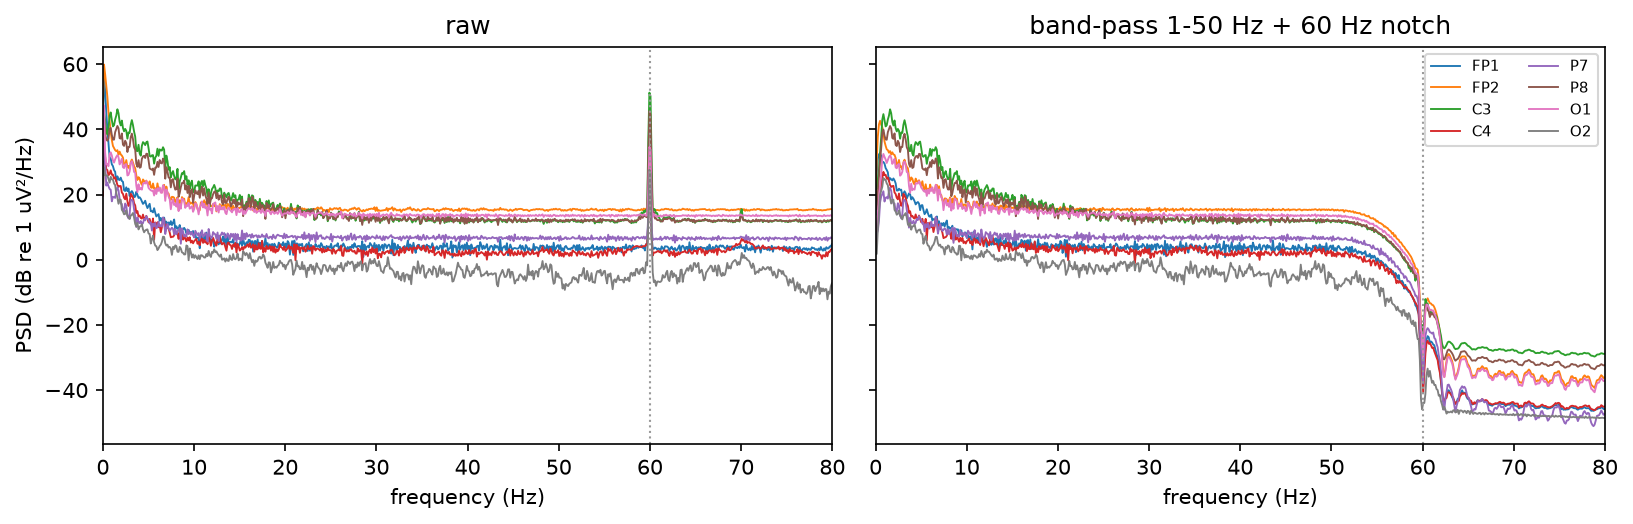
\includegraphics[width=0.94\linewidth]{run1_psd_before_after.png}
  \caption{Run~1 power spectra before filtering (left) and after the 1--50~Hz
  band-pass and 60~Hz notch (right). The dotted line marks 60~Hz.}
  \label{fig:psd}
\end{figure}

\subsection{Statistical implementation}

The first function, \texttt{nonparametric\_test}, accepts arrays with shape
$(n_{\mathrm{epochs}},8,n_{\mathrm{times}})$ and returns each channel's selected
cluster mass and location. It uses \texttt{scipy.stats.ttest\_ind} and
\texttt{scipy.ndimage.label}. The second function,
\texttt{permutation\_test}, pools the conditions, shuffles the trials and splits
them back into groups of their original sizes. We used 1000 random partitions
with seed~0 and a two-sided comparison of absolute cluster masses.

We estimated the permutation tail probability as
\begin{equation}
  \hat p_c=\frac{1}{1000}\sum_{b=1}^{1000}
            \mathbf{1}\!\left(T_c^{(b)}\geq T_c^{\mathrm{obs}}\right).
\end{equation}
For correction across channels, $T_c^{(b)}$ is replaced by
$\max_j T_j^{(b)}$. When no partition exceeded the observed statistic, we
report the count $0/1000$; finite sampling does not establish an exact
$p$-value of zero. We used $\alpha=0.05$.

Simulation checks included a planted effect, a brute-force cluster calculation
and pure-noise data. MNE's cluster-test implementation gave values differing
by at most 0.001. We tested each run separately
and then concatenated their z-scored epochs for the pooled analysis. In the
pooled test, labels were shuffled across all trials without a run restriction.

\section{Results}

\subsection{Data quality}

The cropped recordings contained 90 and 89 trial events, with no additional
sync events. Recorded pulse widths had medians of 120 and 136~ms, longer than
the video's 50~ms marker. Signal quality varied across electrodes
(Table~\ref{tab:quality}). C4 and O2 had lower variability than C3, FP2 and P8.
The raw traces and P8's sharp marker-locked deflection are shown in the
appendices.

\begin{table}[H]
  \centering
  \caption{Trial counts and standard deviations of the cropped, filtered EEG.}
  \label{tab:quality}
  \begin{tabular}{lrr}
    \toprule
     & Run 1 & Run 2 \\
    \midrule
    Matched trials / 90 & 90 & 89 \\
    Circle / square epochs & 15 / 75 & 15 / 74 \\
    Lost samples & 0 & 0 \\
    \midrule
    FP1 SD (\uv) & 38.2 & 85.2 \\
    FP2 SD (\uv) & 100.2 & 119.4 \\
    C3 SD (\uv)  & 239.0 & 130.4 \\
    C4 SD (\uv)  & 25.4 & 24.4 \\
    P7 SD (\uv)  & 16.8 & 35.6 \\
    P8 SD (\uv)  & 145.9 & 150.3 \\
    O1 SD (\uv)  & 59.7 & 28.0 \\
    O2 SD (\uv)  & 17.9 & 17.0 \\
    \bottomrule
  \end{tabular}
\end{table}

\subsection{Main analysis window}

No channel reached the 0.05 threshold in run~1. In run~2, circles were more
negative than squares at C4 from 360 to 500~ms and at O2 from 420 to 500~ms
(Figure~\ref{fig:targets}). The average circle-minus-square differences within
these clusters were $-19.8$ and $-12.9$~\uv, respectively. The pooled analysis
selected negative clusters at the same two channels. Table~\ref{tab:main}
gives the results for all electrodes. No cluster remained below 0.05 after
correction across channels; the smallest corrected value was 0.174.

\begin{table}[H]
  \centering
  \caption{Main-window permutation results. Values in parentheses
  use the maximum statistic across eight channels.}
  \label{tab:main}
  \small
  \begin{tabular}{lccc}
    \toprule
    Channel & Run 1 & Run 2 & Pooled \\
    \midrule
    FP1 & 1.000 (1.000) & 0.577 (0.999) & 1.000 (1.000) \\
    FP2 & 1.000 (1.000) & 0.088 (0.392) & 0.088 (0.338) \\
    C3  & 1.000 (1.000) & 0.145 (0.482) & 1.000 (1.000) \\
    C4  & 0.286 (0.863) & 0.023 (0.174) & 0.044 (0.220) \\
    P7  & 0.104 (0.526) & 0.594 (0.996) & 0.465 (0.970) \\
    P8  & 0.596 (0.992) & 1.000 (1.000) & 0.436 (0.953) \\
    O1  & 0.462 (0.947) & 0.322 (0.859) & 0.315 (0.835) \\
    O2  & 0.157 (0.678) & 0.006 (0.230) & 0.017 (0.179) \\
    \bottomrule
  \end{tabular}
\end{table}

\begin{figure}[H]
  \centering
  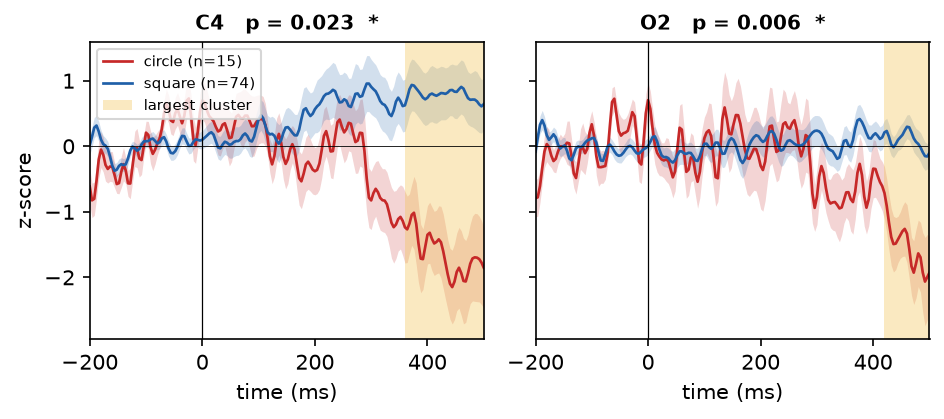
\includegraphics[width=0.79\linewidth]{run2_main_erp_significant.png}
  \par\smallskip
  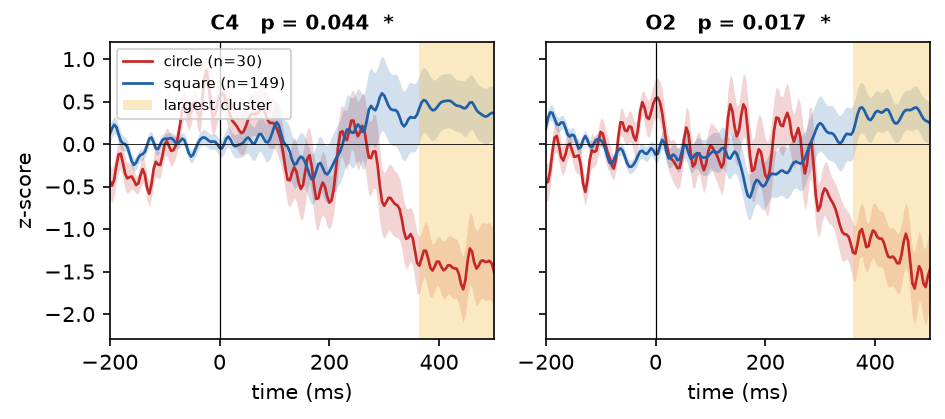
\includegraphics[width=0.79\linewidth]{pooled_main_erp_significant.png}
  \caption{Main-window responses at C4 and O2 in run~2 (top) and pooled data
  (bottom). Red: circles; blue: squares. Bands around the means show SEM;
  yellow marks the selected cluster. Title values are channel-wise,
  without correction across channels.}
  \label{fig:targets}
\end{figure}

\subsection{Extended analysis window}

With the longer epochs, run~2's O2 cluster extended to 580~ms and none of the
1000 sampled partitions exceeded its observed mass. The pooled O2 cluster
extended to 576~ms. Run~2 also had negative clusters at C4 and C3; pooled C4
was above the channel-wise threshold (Table~\ref{tab:extended}). Run~1 again
had no channel below 0.05. Across all extended-window results, the smallest
channel-corrected value was 0.116. The extended-window waveforms are shown in
Appendix~\ref{app:extendedplots}.

\begin{table}[H]
  \centering
  \caption{Selected extended-window clusters. The table includes channels
  below 0.05 in either run~2 or the pooled analysis; full results appear in
  Appendix~\ref{app:stats}. Negative mass means circles below squares.}
  \label{tab:extended}
  \small
  \begin{tabular}{llrrrr}
    \toprule
    Data & Channel & Window (ms) & $\sum t$ & $\hat p$ & Corrected \\
    \midrule
    Run 2 & C3 & $484$ to $628$ & $-93.65$ & 0.035 & 0.245 \\
    Run 2 & C4 & $360$ to $556$ & $-126.12$ & 0.022 & 0.162 \\
    Run 2 & O2 & $420$ to $580$ & $-152.63$ & $0/1000$ & 0.123 \\
    Pooled & C3 & --- & 0 & 1.000 & 1.000 \\
    Pooled & C4 & $364$ to $512$ & $-92.91$ & 0.059 & 0.284 \\
    Pooled & O2 & $360$ to $576$ & $-153.68$ & 0.009 & 0.116 \\
    \bottomrule
  \end{tabular}
\end{table}

\section{Discussion}

The late negative difference at O2 and C4 does not match the expected positive
P300. Our montage lacked Pz and Cz, the sites closest to its usual maximum
\cite{polich}. Only circles required a button press, so motor activity is
part of the condition contrast. Colour and shape also differed. These
factors limit how specifically we can interpret the target response.

C3, FP2 and P8 showed much larger fluctuations than the cleaner channels.
In the extended window, C3's selected cluster had a mean voltage difference
of $-122.1$~\uv. Its size and the noisy traces raise concern about artefact
contamination. P8's sharp marker-locked deflection also warrants a hardware
check. Electrical pickup is one possible source, but its origin and the
photoresistor's onset delay were not measured.

The pooled analysis contains run~2 and therefore provides no independent
replication. Its unrestricted shuffling also assumes exchangeability between
runs. A follow-up analysis could shuffle labels within each run to preserve
run-specific noise distributions. More recordings would help assess whether
the effect persists beyond this participant and session.

The next useful check would be to repeat the analysis after identifying noisy
trials, using the same rejection rule for both conditions. During recording,
checking electrode contact and marker latency, keeping marker wiring away
from EEG leads, and recording button presses would address the main sources
of uncertainty in these data.

\section{Conclusion}

Run~2 showed a late target-related negativity at O2 and C4. Run~1 did not
show a significant channel-wise difference, and no result survived correction
across eight channels. The findings remain exploratory because of the
limited recordings, recording noise and confounded condition contrast.

\begin{thebibliography}{9}
\bibitem{maris}
Maris, E., and Oostenveld, R. (2007).
Nonparametric statistical testing of EEG- and MEG-data.
\emph{Journal of Neuroscience Methods}, 164(1), 177--190.
\href{https://doi.org/10.1016/j.jneumeth.2007.03.024}{doi:10.1016/j.jneumeth.2007.03.024}.

\bibitem{mne}
Gramfort, A., et al. (2013).
MEG and EEG data analysis with MNE-Python.
\emph{Frontiers in Neuroscience}, 7, 267.
\href{https://doi.org/10.3389/fnins.2013.00267}{doi:10.3389/fnins.2013.00267}.

\bibitem{polich}
Polich, J. (2007).
Updating P300: An integrative theory of P3a and P3b.
\emph{Clinical Neurophysiology}, 118(10), 2128--2148.
\href{https://doi.org/10.1016/j.clinph.2007.04.019}{doi:10.1016/j.clinph.2007.04.019}.
\end{thebibliography}

\clearpage
\appendix
\section{Event alignment and raw traces}
\label{app:quality}

\begin{figure}[htbp]
  \centering
  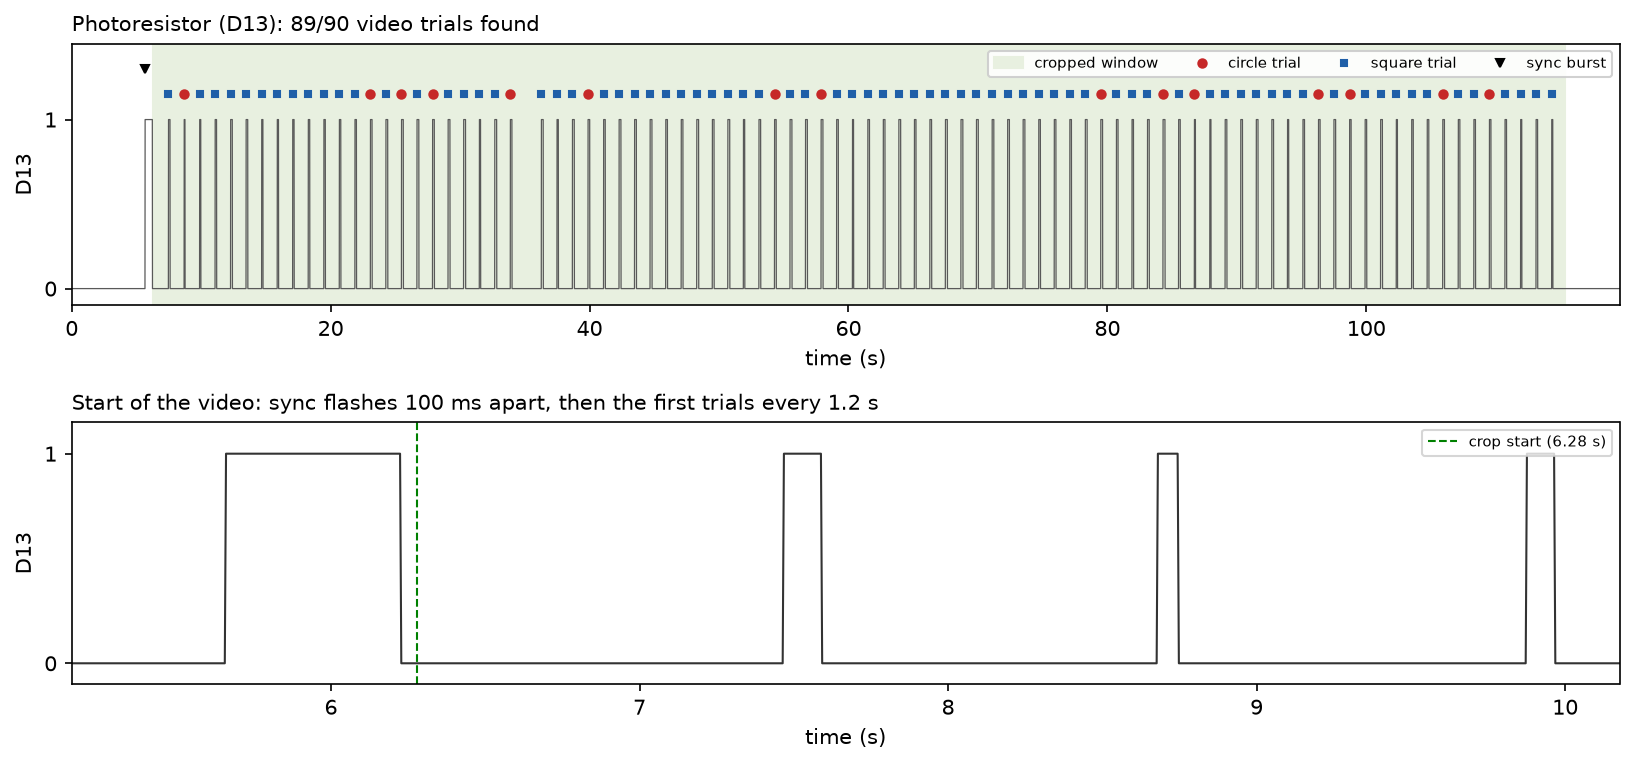
\includegraphics[width=0.94\linewidth]{run2_photoresistor.png}
  \caption{Run~2 event alignment. The upper panel shows D13 and the matched
  circle and square trials; the lower panel expands the start of the video.
  Five sync flashes appear as one recorded pulse. Trial~24's marker was missed.}
  \label{fig:alignment}
\end{figure}

\begin{figure}[htbp]
  \centering
  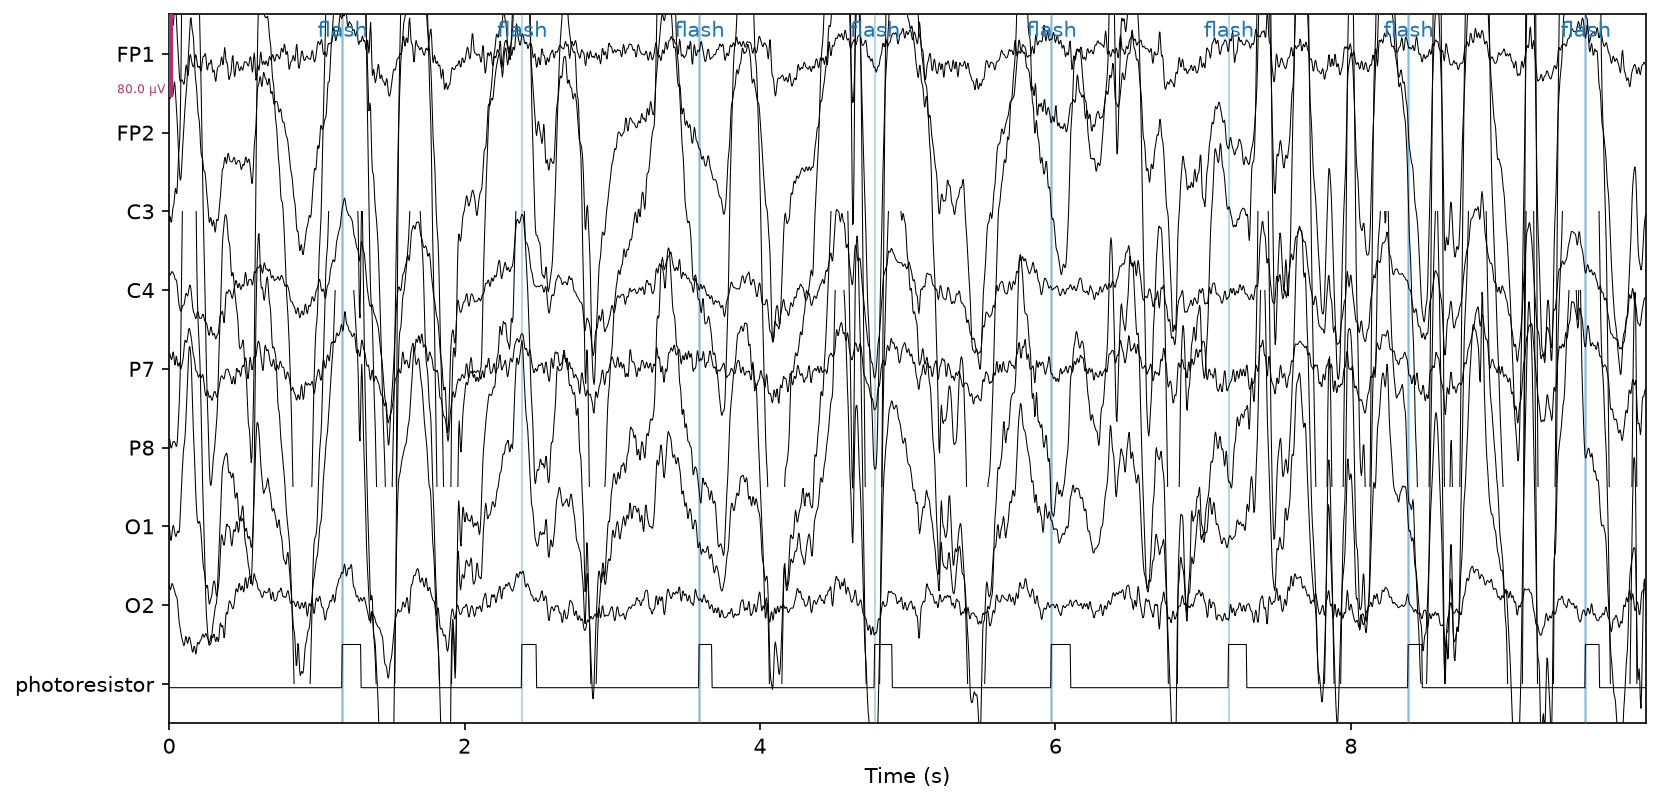
\includegraphics[width=0.94\linewidth]{run1_raw_annotations.png}
  \caption{First 10~s of cropped, filtered run~1 with event annotations and
  the D13 trace. The displayed EEG scale bar is 80~\uv. C3, FP2 and P8 have
  larger fluctuations than C4 and O2.}
  \label{fig:raw}
\end{figure}

\FloatBarrier
\clearpage
\section{Responses across all channels}
\label{app:allchannels}

\begin{figure}[htbp]
  \centering
  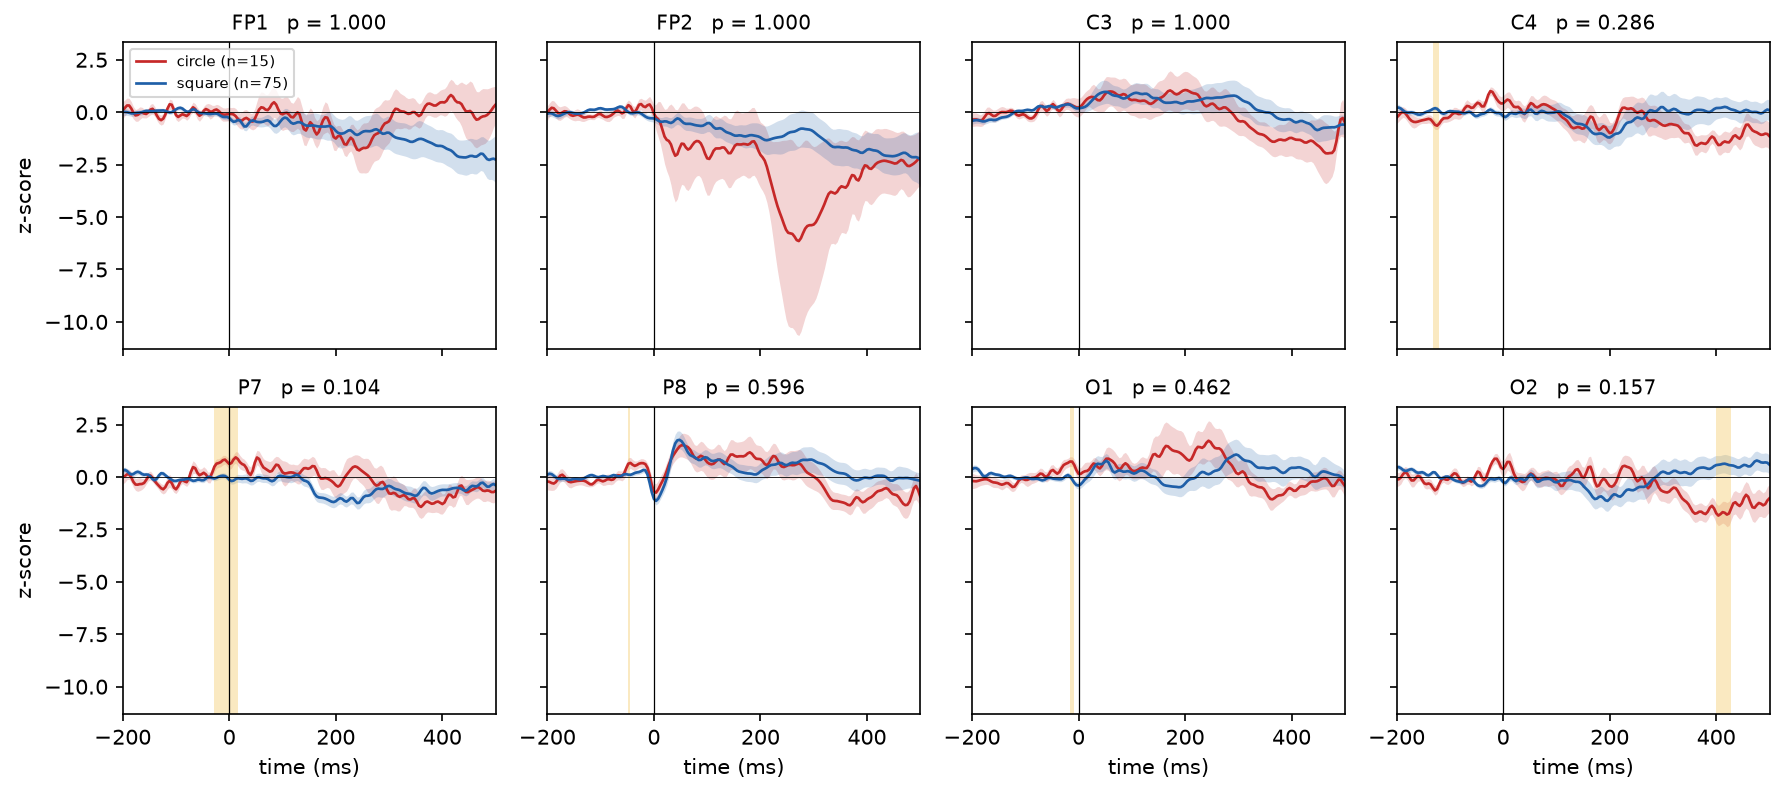
\includegraphics[width=0.94\linewidth]{run1_main_erp_all.png}
  \caption{Run~1 main-window responses: 15 circle and 75 square trials.
  Red and blue curves show means with SEM. Yellow marks each channel's
  selected cluster, including clusters above the permutation threshold.}
\end{figure}

\begin{figure}[htbp]
  \centering
  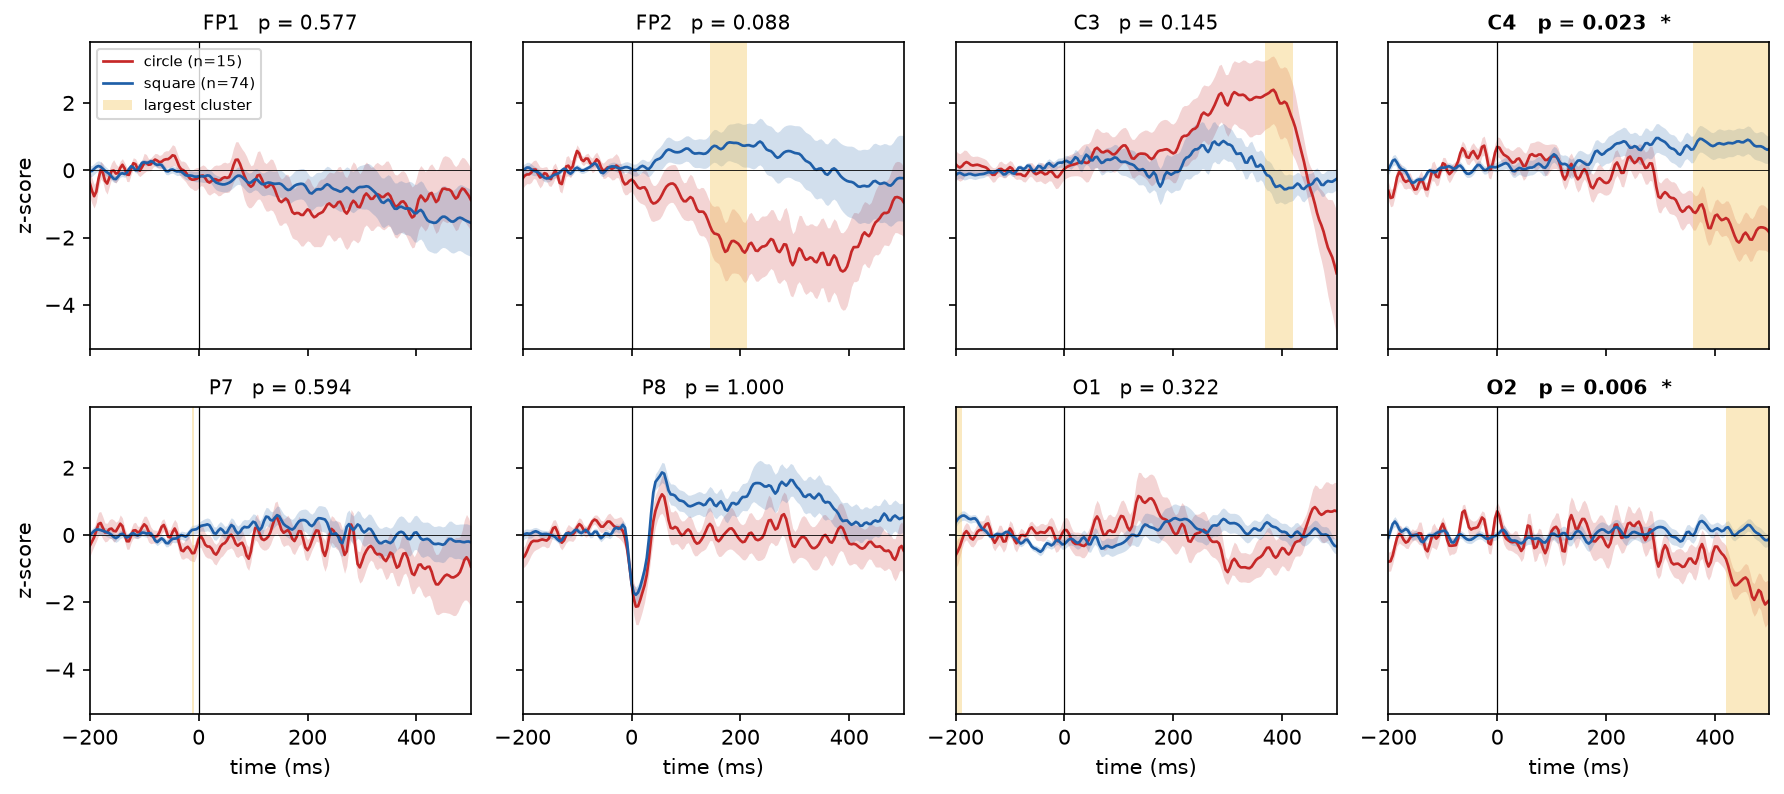
\includegraphics[width=0.94\linewidth]{run2_main_erp_all.png}
  \caption{Run~2 main-window responses: 15 circle and 74 square trials.
  Plot conventions are as above. Title values are channel-wise.}
\end{figure}

\clearpage
\begin{figure}[htbp]
  \centering
  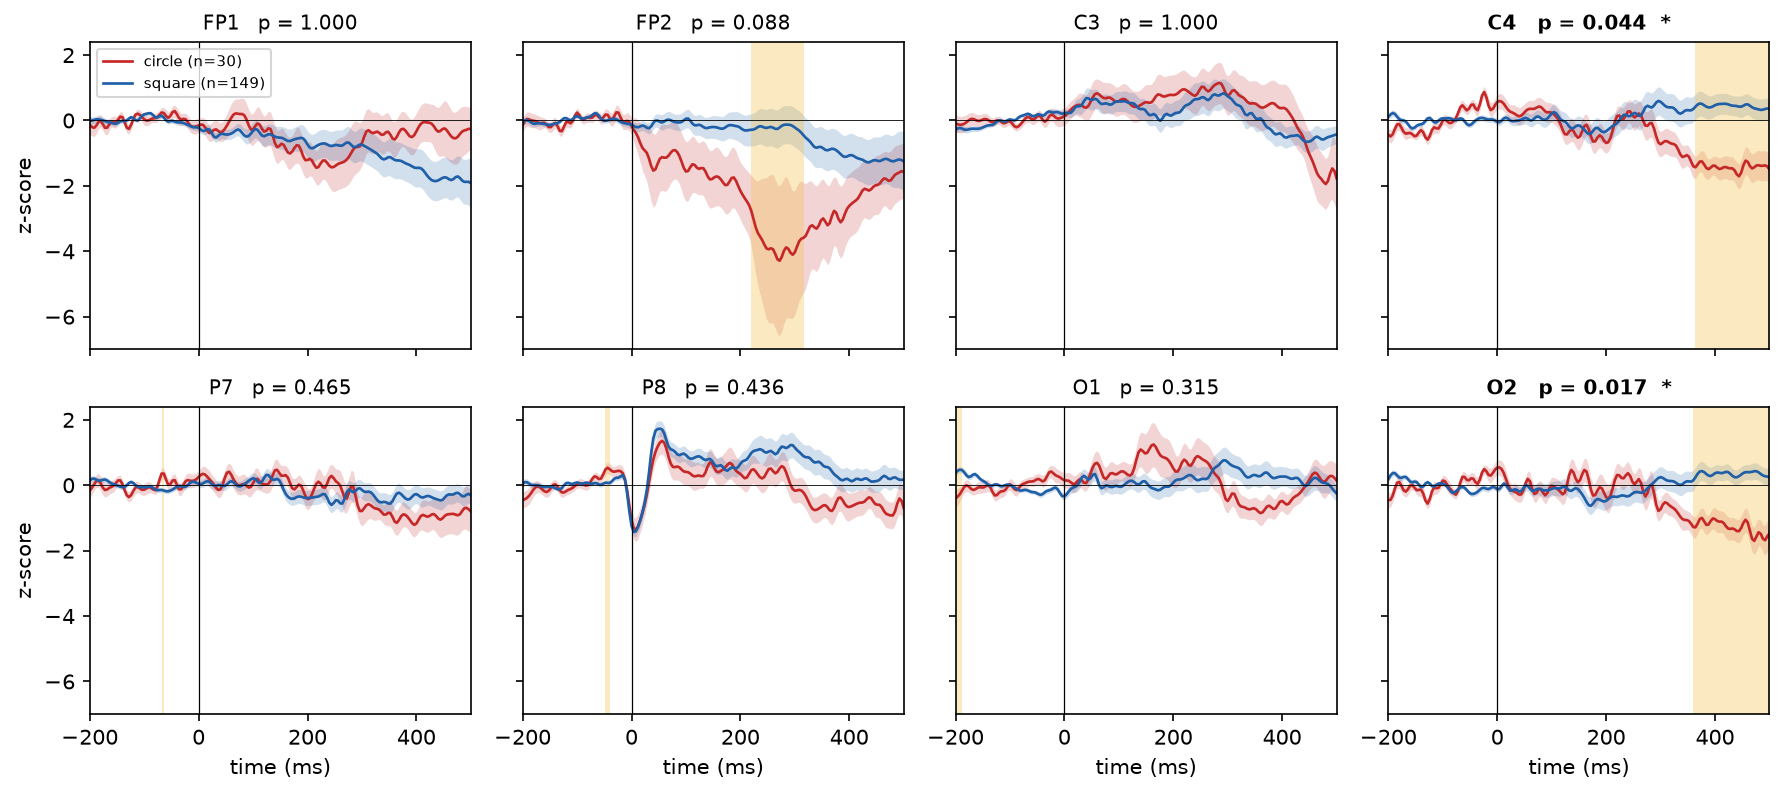
\includegraphics[width=0.94\linewidth]{pooled_main_erp_all.png}
  \caption{Pooled main-window responses: 30 circle and 149 square trials.}
\end{figure}

\begin{figure}[htbp]
  \centering
  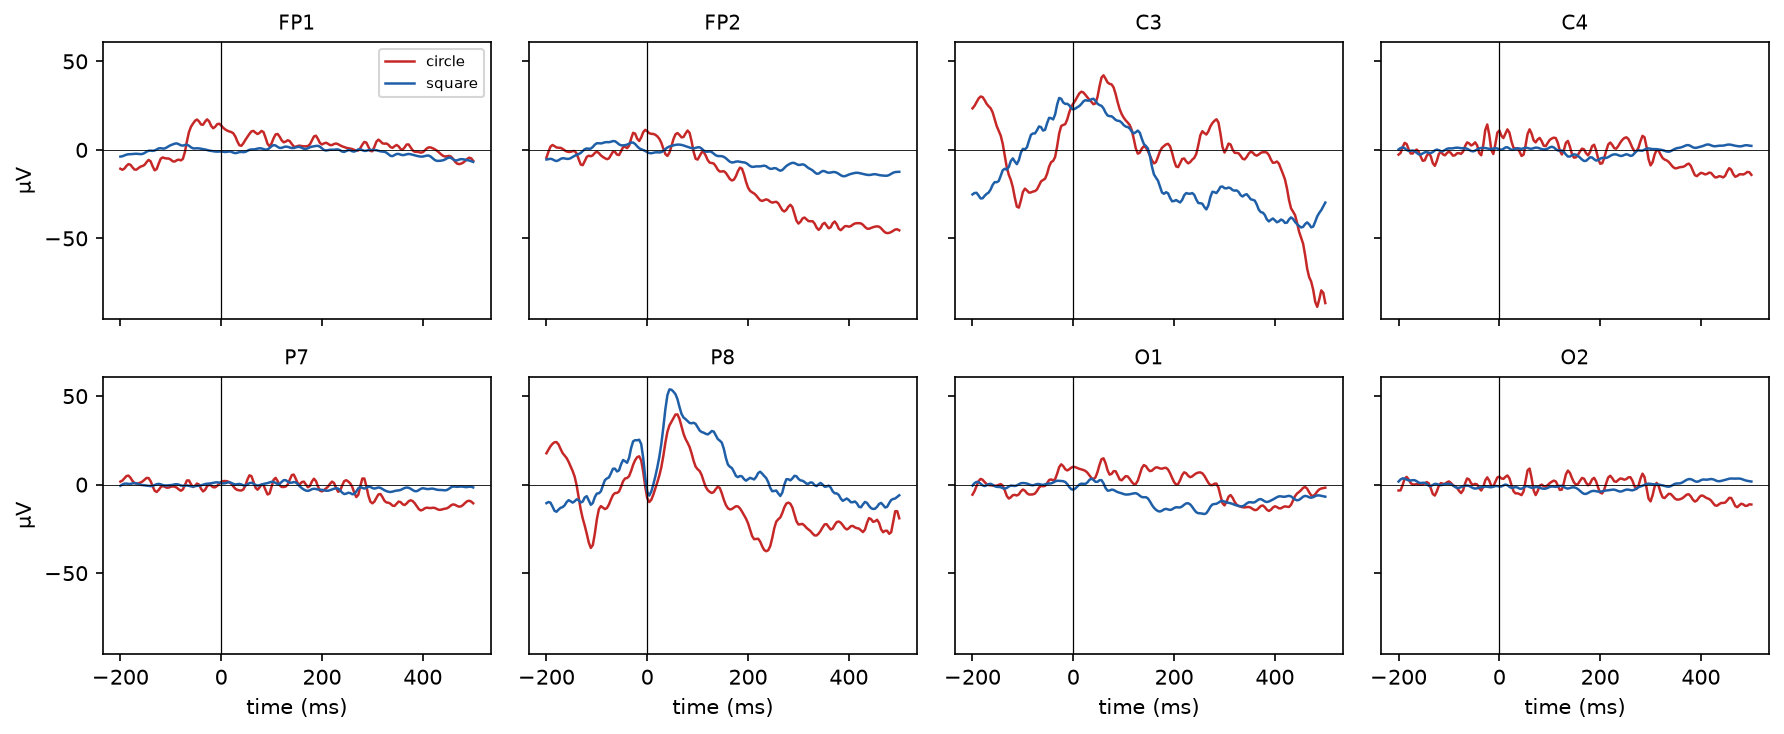
\includegraphics[width=0.94\linewidth]{pooled_evoked_microvolts.png}
  \caption{Pooled baseline-corrected averages in microvolts, without
  baseline-standard-deviation scaling.}
\end{figure}

\FloatBarrier
\clearpage
\section{Extended-window responses}
\label{app:extendedplots}

\begin{figure}[H]
  \centering
  \begin{minipage}{0.96\linewidth}
    \centering
    % Replace only the raster titles; retain all axes and waveform data.
    % Image dimensions are 1423 x 419 pixels (height/width = 0.29445).
    \setlength{\unitlength}{\linewidth}
    \begin{picture}(1,0.29445)
      \put(0,0){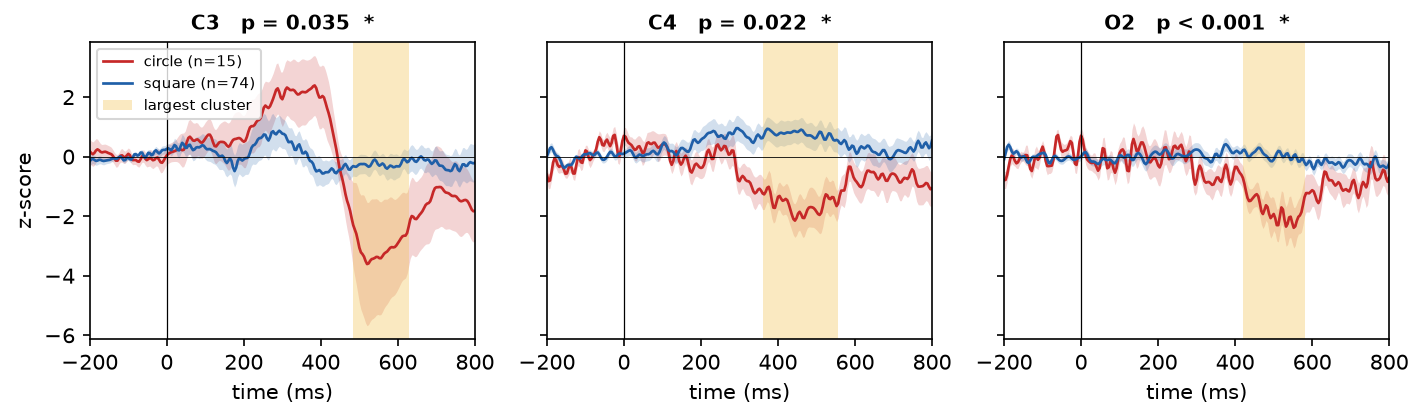
\includegraphics[width=\linewidth]{run2_extended_erp_significant.png}}
      \put(0,0.267){\color{white}\rule{\linewidth}{0.028\linewidth}}
      \put(0.20,0.280){\makebox(0,0){\small C3: $\hat p=0.035$}}
      \put(0.52,0.280){\makebox(0,0){\small C4: $\hat p=0.022$}}
      \put(0.84,0.280){\makebox(0,0){\small O2: $0/1000$}}
    \end{picture}
  \end{minipage}
  \caption{Run~2 responses over $-0.2$ to $0.8$~s at the three channels
  below the channel-wise threshold. Circles are red and squares blue;
  bands show SEM and yellow marks the selected cluster. For O2, none of
  the 1000 sampled partitions exceeded the observed mass. No channel
  survived correction across eight electrodes.}
  \label{fig:run2extended}
\end{figure}

\begin{figure}[H]
  \centering
  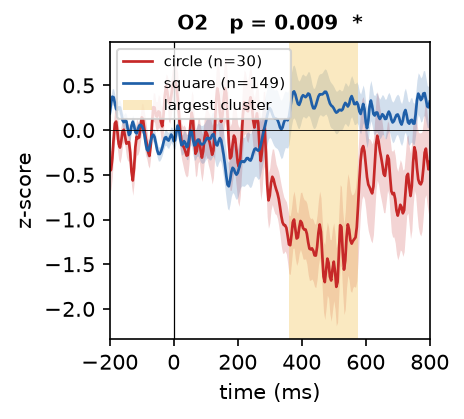
\includegraphics[width=0.46\linewidth]{pooled_extended_erp_significant.png}
  \caption{Pooled O2 responses over $-0.2$ to $0.8$~s, with 30 circle and
  149 square epochs. The channel-wise exceedance fraction is 0.009;
  after correction across eight electrodes it is 0.116. Plot conventions
  are as above.}
  \label{fig:pooledextended}
\end{figure}

\FloatBarrier
\clearpage
\section{Full cluster statistics}
\label{app:stats}

% These tables are generated from the original report/results.json.
% The empirical fractions and the analysis code have not been altered.
\footnotesize
\renewcommand{\arraystretch}{1.0}
\begin{table}[!htbp]
\centering
\caption{Main window: $-0.2$ to $0.5$~s. A dash indicates that no cluster crossed the sample-level threshold.}
\begin{tabular}{llrrrr}
\toprule
Data & Channel & Window (ms) & $\sum t$ & $\hat p$ & Corrected \\
\midrule
Run 1 & FP1 & --- & 0.00 & 1.000 & 1.000 \\
 & FP2 & --- & 0.00 & 1.000 & 1.000 \\
 & C3 & --- & 0.00 & 1.000 & 1.000 \\
 & C4 & $-132$ to $-120$ & -10.46 & 0.286 & 0.863 \\
 & P7 & $-28$ to $16$ & 27.07 & 0.104 & 0.526 \\
 & P8 & $-48$ to $-44$ & 4.16 & 0.596 & 0.992 \\
 & O1 & $-16$ to $-8$ & 7.03 & 0.462 & 0.947 \\
 & O2 & $400$ to $428$ & -18.14 & 0.157 & 0.678 \\
\addlinespace[5pt]
Run 2 & FP1 & $-192$ to $-192$ & -2.09 & 0.577 & 0.999 \\
 & FP2 & $144$ to $212$ & -40.46 & 0.088 & 0.392 \\
 & C3 & $368$ to $420$ & 31.58 & 0.145 & 0.482 \\
 & C4 & $360$ to $500$ & -92.68 & 0.023 & 0.174 \\
 & P7 & $-12$ to $-8$ & -4.30 & 0.594 & 0.996 \\
 & P8 & --- & 0.00 & 1.000 & 1.000 \\
 & O1 & $-200$ to $-188$ & -9.97 & 0.322 & 0.859 \\
 & O2 & $420$ to $500$ & -71.91 & 0.006 & 0.230 \\
\addlinespace[5pt]
Pooled & FP1 & --- & 0.00 & 1.000 & 1.000 \\
 & FP2 & $220$ to $316$ & -57.80 & 0.088 & 0.338 \\
 & C3 & --- & 0.00 & 1.000 & 1.000 \\
 & C4 & $364$ to $500$ & -85.50 & 0.044 & 0.220 \\
 & P7 & $-68$ to $-64$ & 5.77 & 0.465 & 0.970 \\
 & P8 & $-48$ to $-40$ & 6.75 & 0.436 & 0.953 \\
 & O1 & $-200$ to $-188$ & -11.68 & 0.315 & 0.835 \\
 & O2 & $360$ to $500$ & -100.65 & 0.017 & 0.179 \\
\bottomrule
\end{tabular}
\end{table}

\begin{table}[!htbp]
\centering
\caption{Extended window: $-0.2$ to $0.8$~s. A dash indicates that no cluster crossed the sample-level threshold.}
\begin{tabular}{llrrrr}
\toprule
Data & Channel & Window (ms) & $\sum t$ & $\hat p$ & Corrected \\
\midrule
Run 1 & FP1 & --- & 0.00 & 1.000 & 1.000 \\
 & FP2 & --- & 0.00 & 1.000 & 1.000 \\
 & C3 & --- & 0.00 & 1.000 & 1.000 \\
 & C4 & $-132$ to $-120$ & -10.46 & 0.384 & 0.942 \\
 & P7 & $-28$ to $16$ & 27.07 & 0.157 & 0.704 \\
 & P8 & $-48$ to $-44$ & 4.16 & 0.695 & 0.998 \\
 & O1 & $-16$ to $-8$ & 7.03 & 0.568 & 0.979 \\
 & O2 & $400$ to $428$ & -18.14 & 0.205 & 0.822 \\
\addlinespace[5pt]
Run 2 & FP1 & $-192$ to $-192$ & -2.09 & 0.609 & 0.999 \\
 & FP2 & $144$ to $212$ & -40.46 & 0.126 & 0.530 \\
 & C3 & $484$ to $628$ & -93.65 & 0.035 & 0.245 \\
 & C4 & $360$ to $556$ & -126.12 & 0.022 & 0.162 \\
 & P7 & $-12$ to $-8$ & -4.30 & 0.615 & 0.997 \\
 & P8 & --- & 0.00 & 1.000 & 1.000 \\
 & O1 & $-200$ to $-188$ & -9.97 & 0.401 & 0.920 \\
 & O2 & $420$ to $580$ & -152.63 & $0/1000$ & 0.123 \\
\addlinespace[5pt]
Pooled & FP1 & --- & 0.00 & 1.000 & 1.000 \\
 & FP2 & $220$ to $316$ & -57.80 & 0.130 & 0.481 \\
 & C3 & --- & 0.00 & 1.000 & 1.000 \\
 & C4 & $364$ to $512$ & -92.91 & 0.059 & 0.284 \\
 & P7 & $-68$ to $-64$ & 5.77 & 0.526 & 0.991 \\
 & P8 & $-48$ to $-40$ & 6.75 & 0.535 & 0.980 \\
 & O1 & $-200$ to $-188$ & -11.68 & 0.426 & 0.920 \\
 & O2 & $360$ to $576$ & -153.68 & 0.009 & 0.116 \\
\bottomrule
\end{tabular}
\end{table}


\clearpage
\normalsize
\section{Code: lab4\_stats.py}
\label{app:statscode}
\begin{figure}[H]
  \centering
  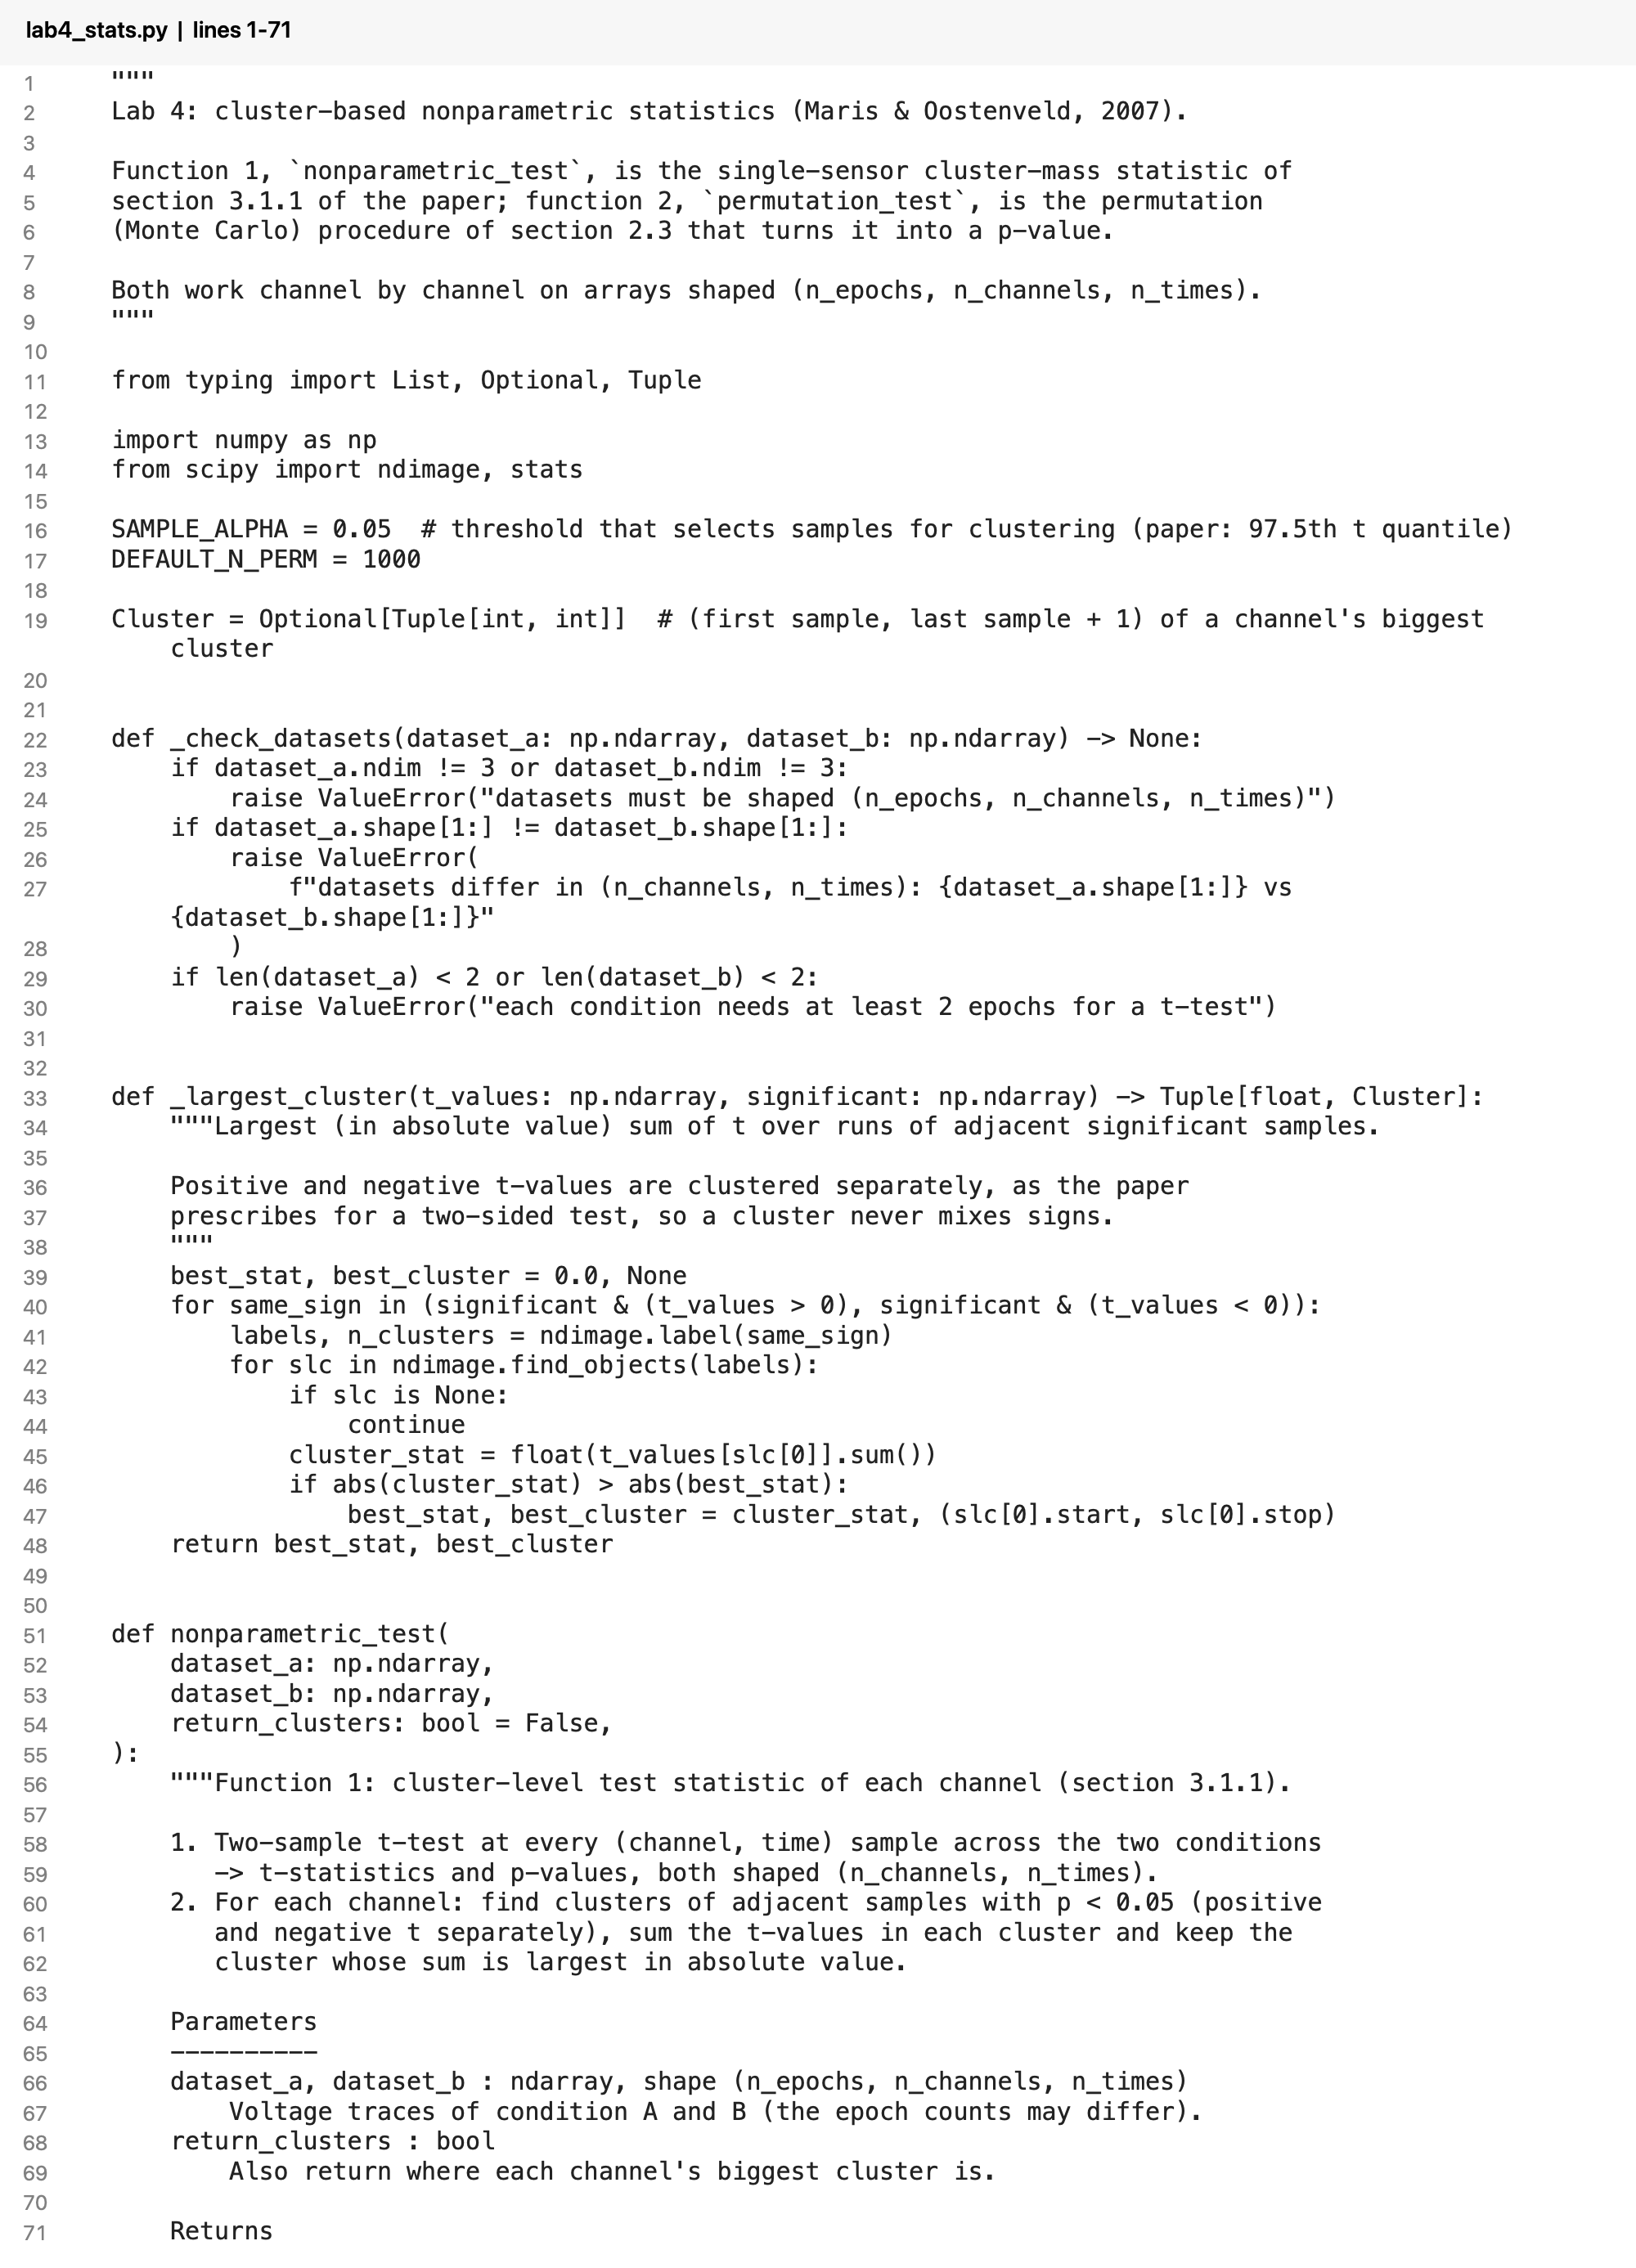
\includegraphics[width=\linewidth,height=0.84\textheight,keepaspectratio]{code_screenshots/stats-01.png}
  \caption{\texttt{lab4\_stats.py}, lines 1--71.}
\end{figure}
\clearpage
\begin{figure}[H]
  \centering
  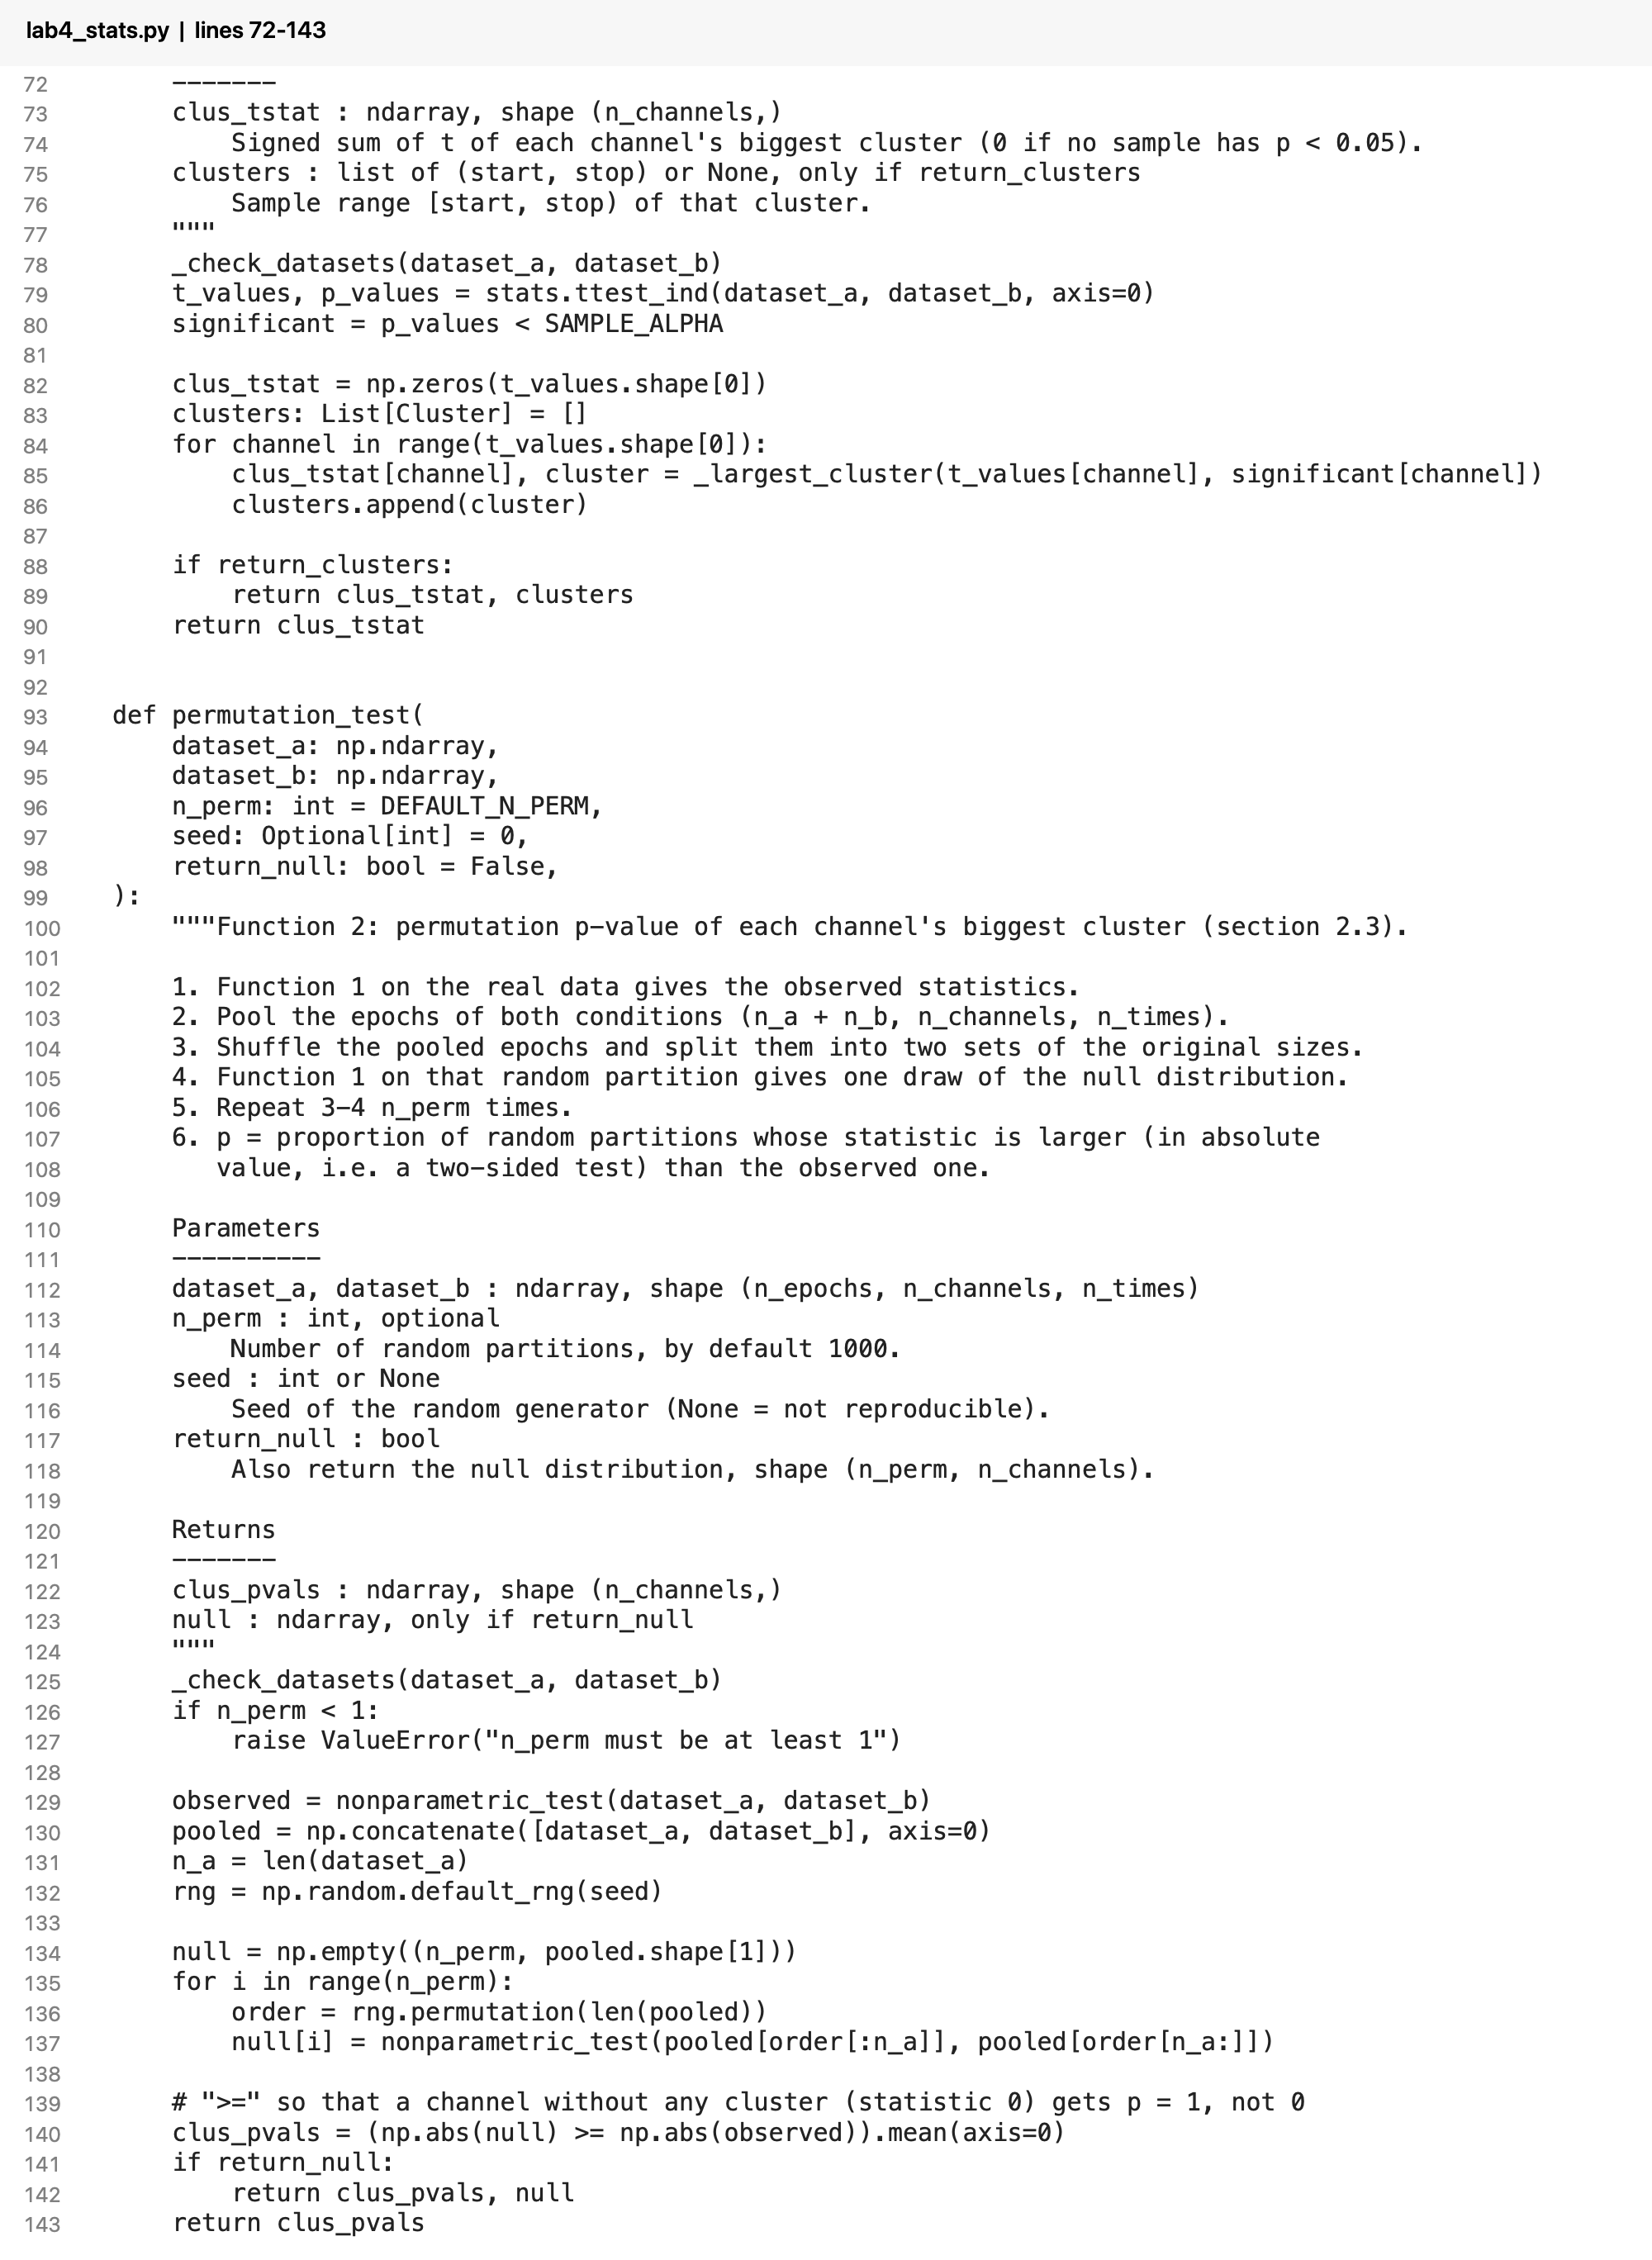
\includegraphics[width=\linewidth,height=0.92\textheight,keepaspectratio]{code_screenshots/stats-02.png}
  \caption{\texttt{lab4\_stats.py}, lines 72--143.}
\end{figure}

\clearpage
\normalsize
\section{Code: lab4\_analysis.py}
\label{app:analysiscode}
\begin{figure}[H]
  \centering
  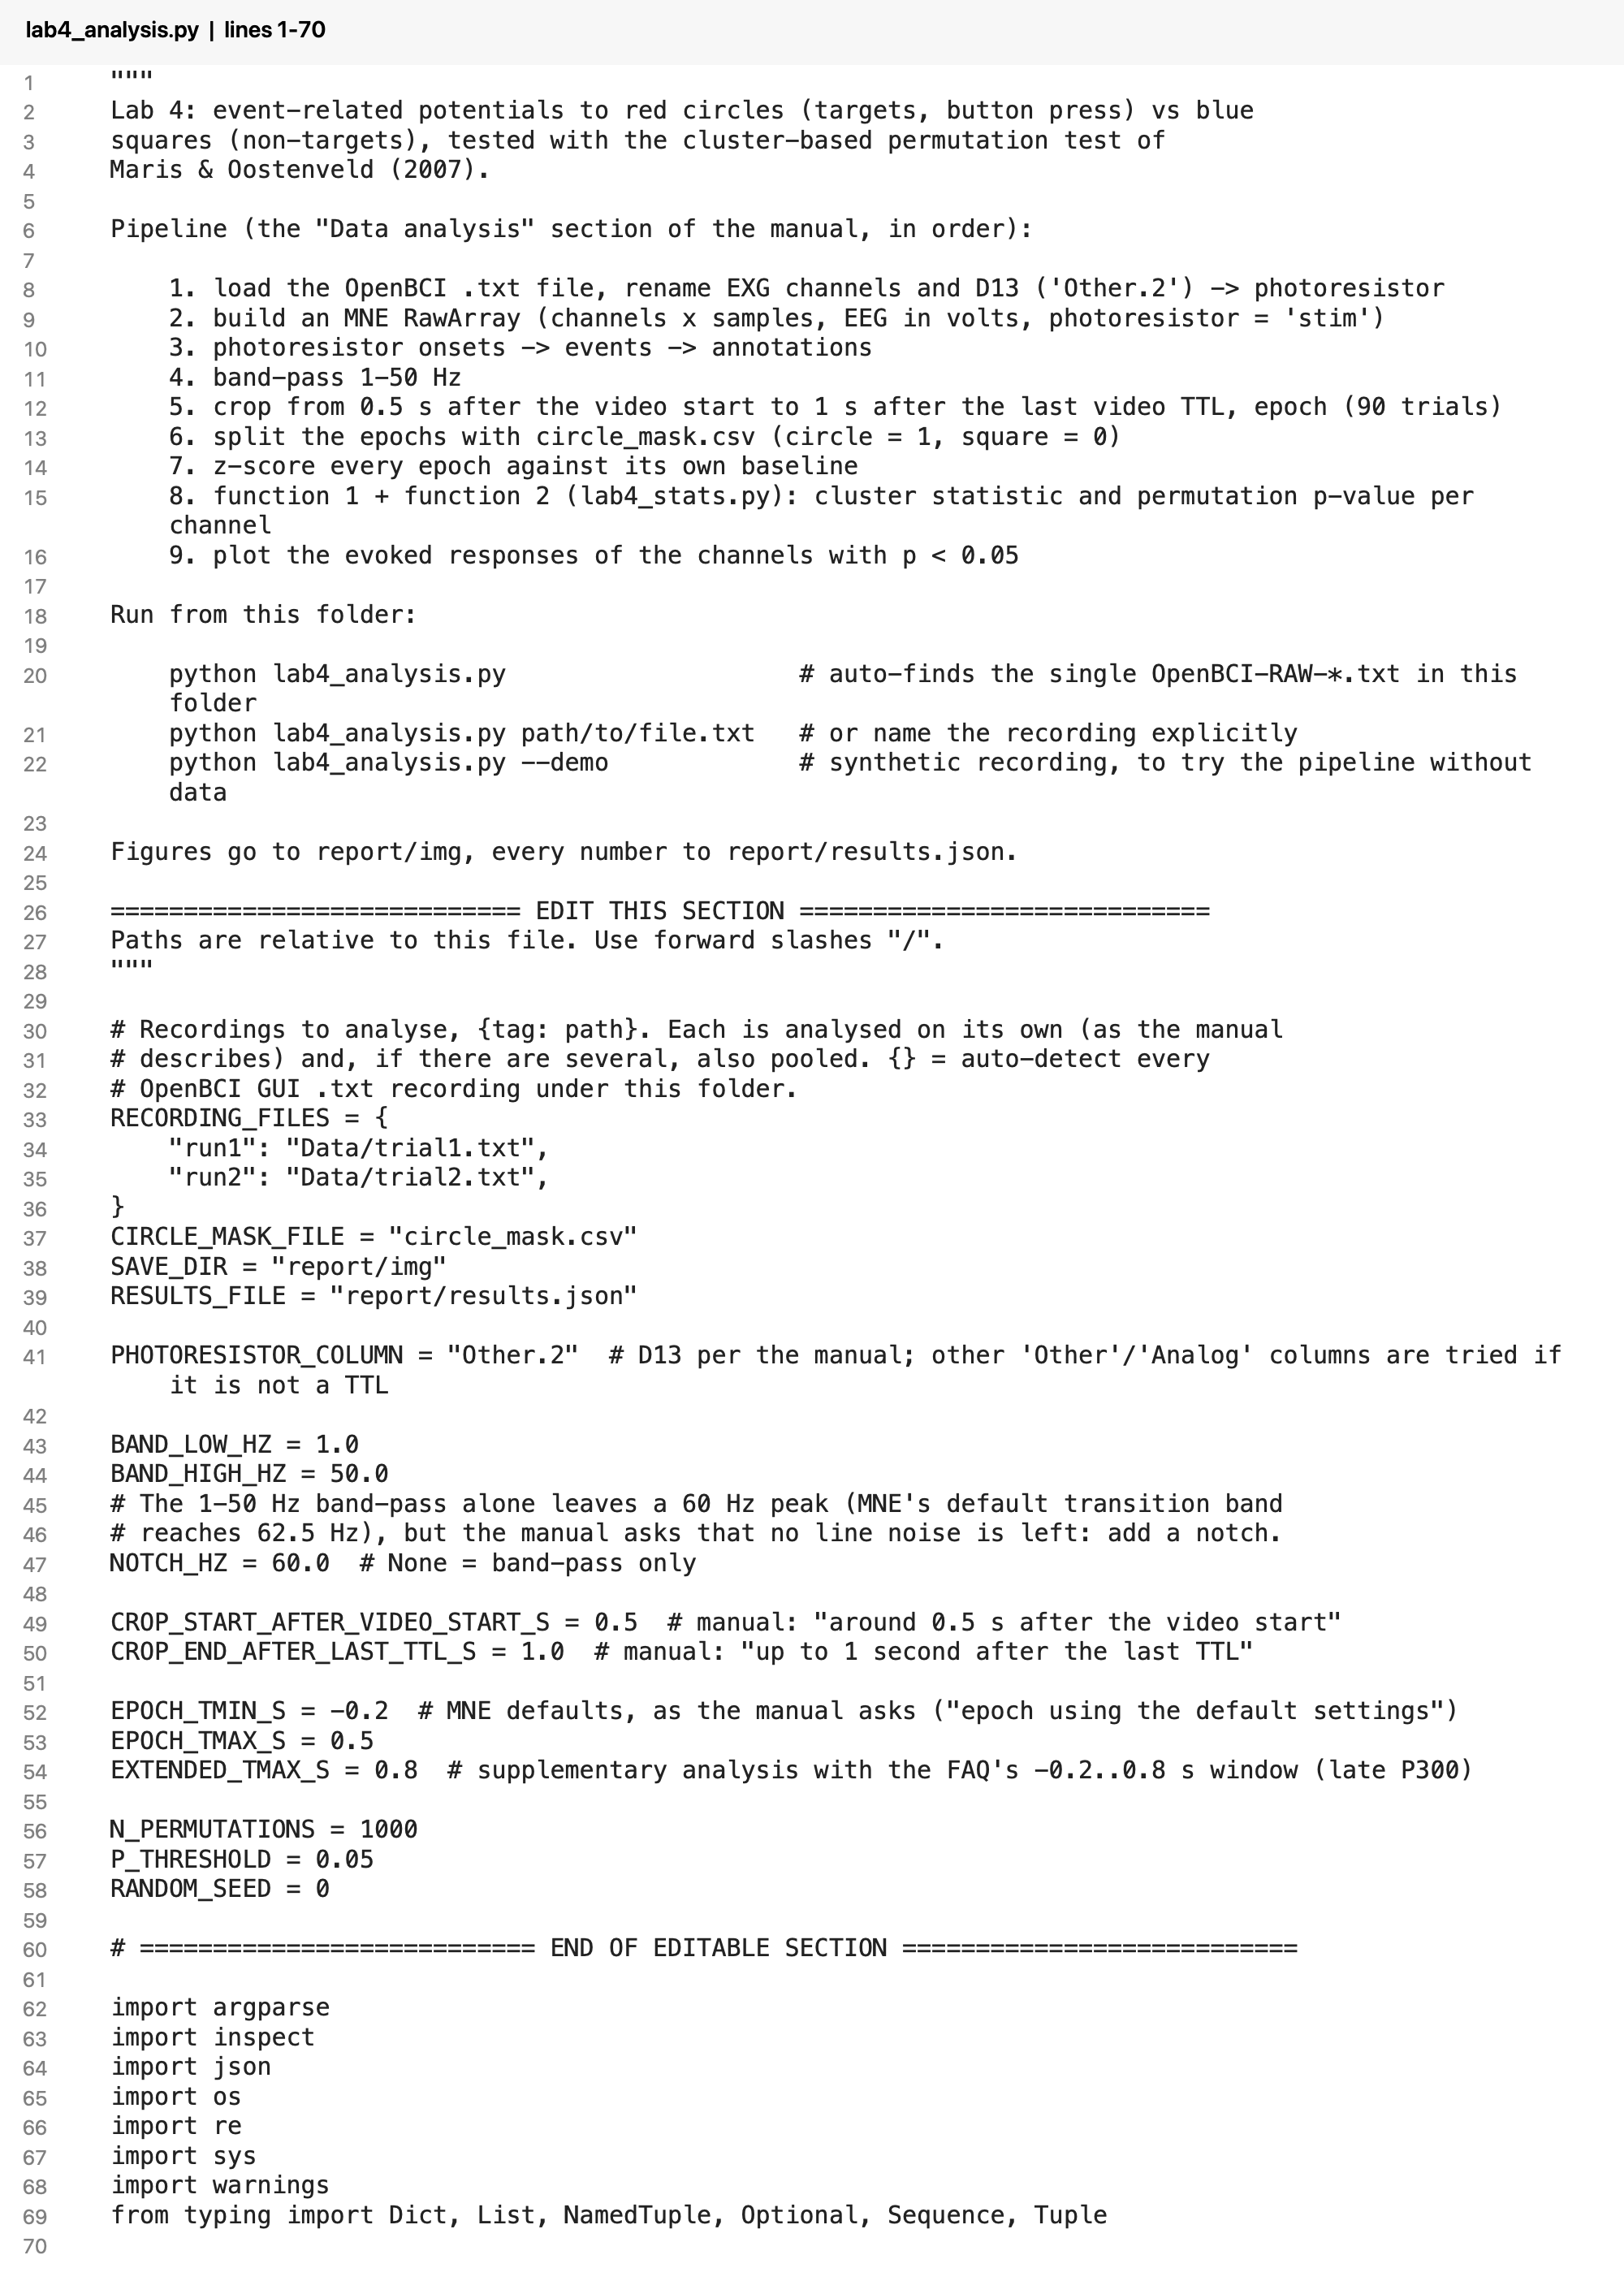
\includegraphics[width=\linewidth,height=0.84\textheight,keepaspectratio]{code_screenshots/analysis-01.png}
  \caption{\texttt{lab4\_analysis.py}, lines 1--70.}
\end{figure}
\clearpage
\begin{figure}[H]
  \centering
  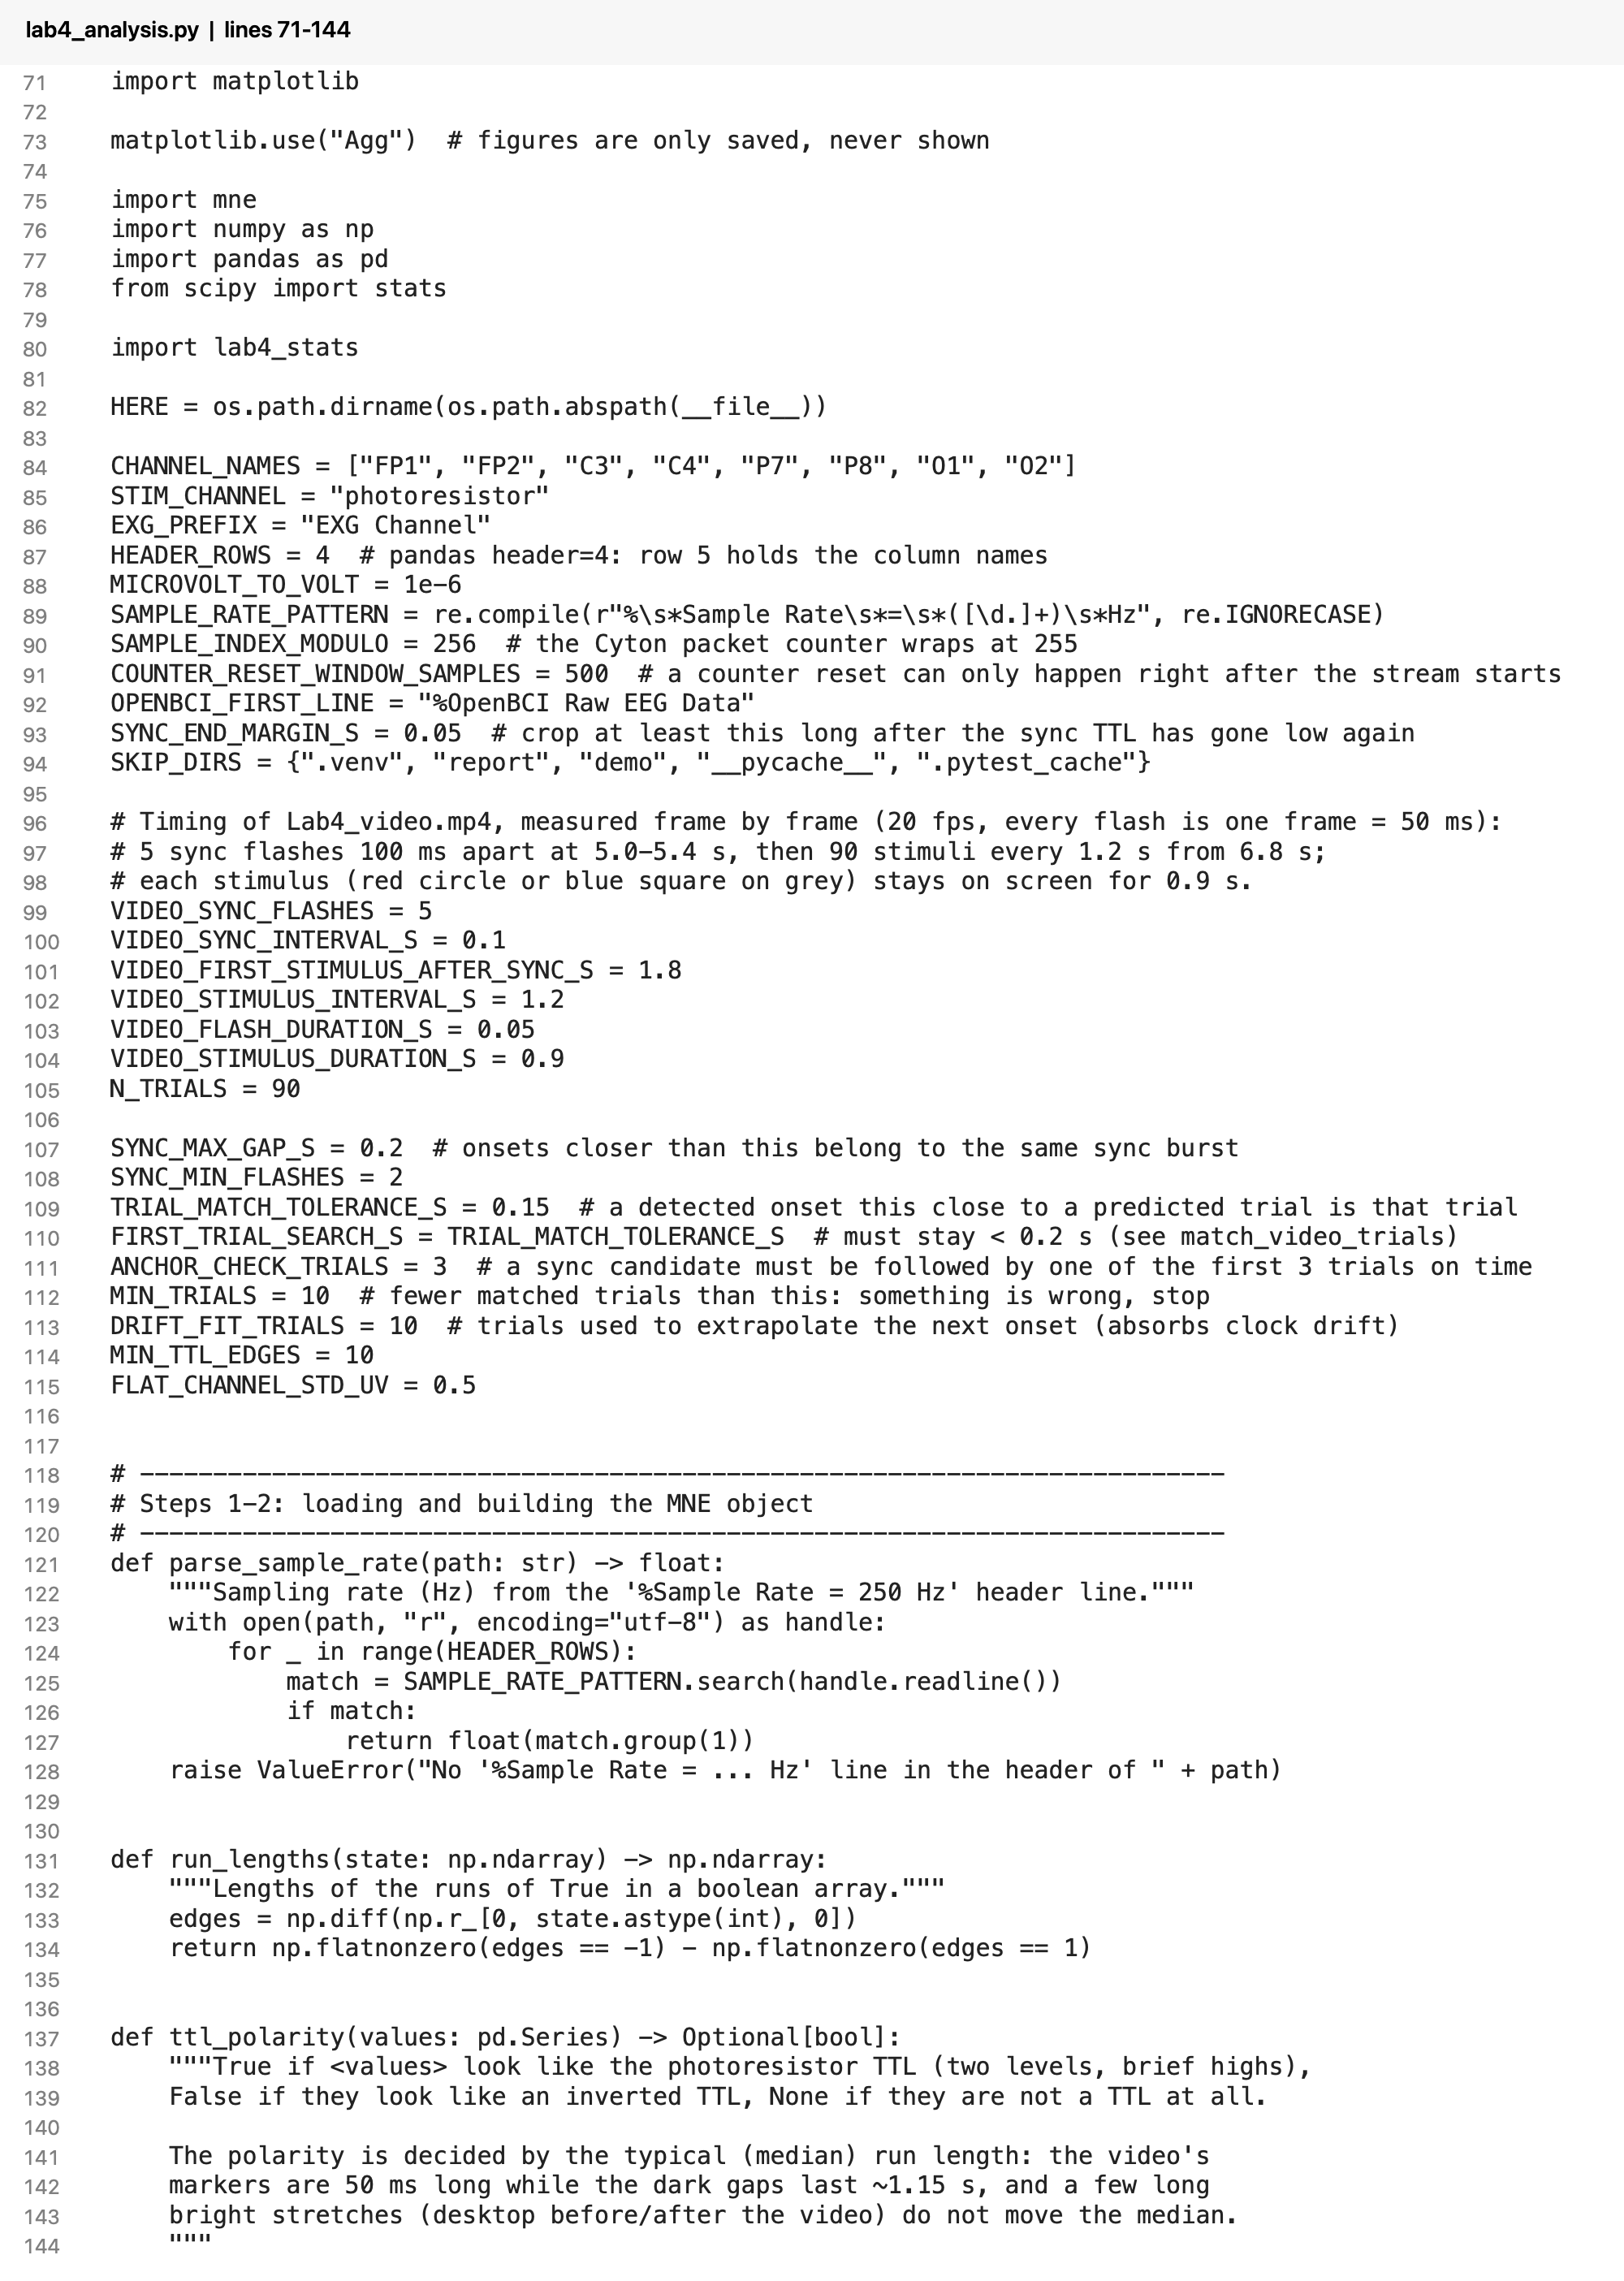
\includegraphics[width=\linewidth,height=0.92\textheight,keepaspectratio]{code_screenshots/analysis-02.png}
  \caption{\texttt{lab4\_analysis.py}, lines 71--144.}
\end{figure}
\clearpage
\begin{figure}[H]
  \centering
  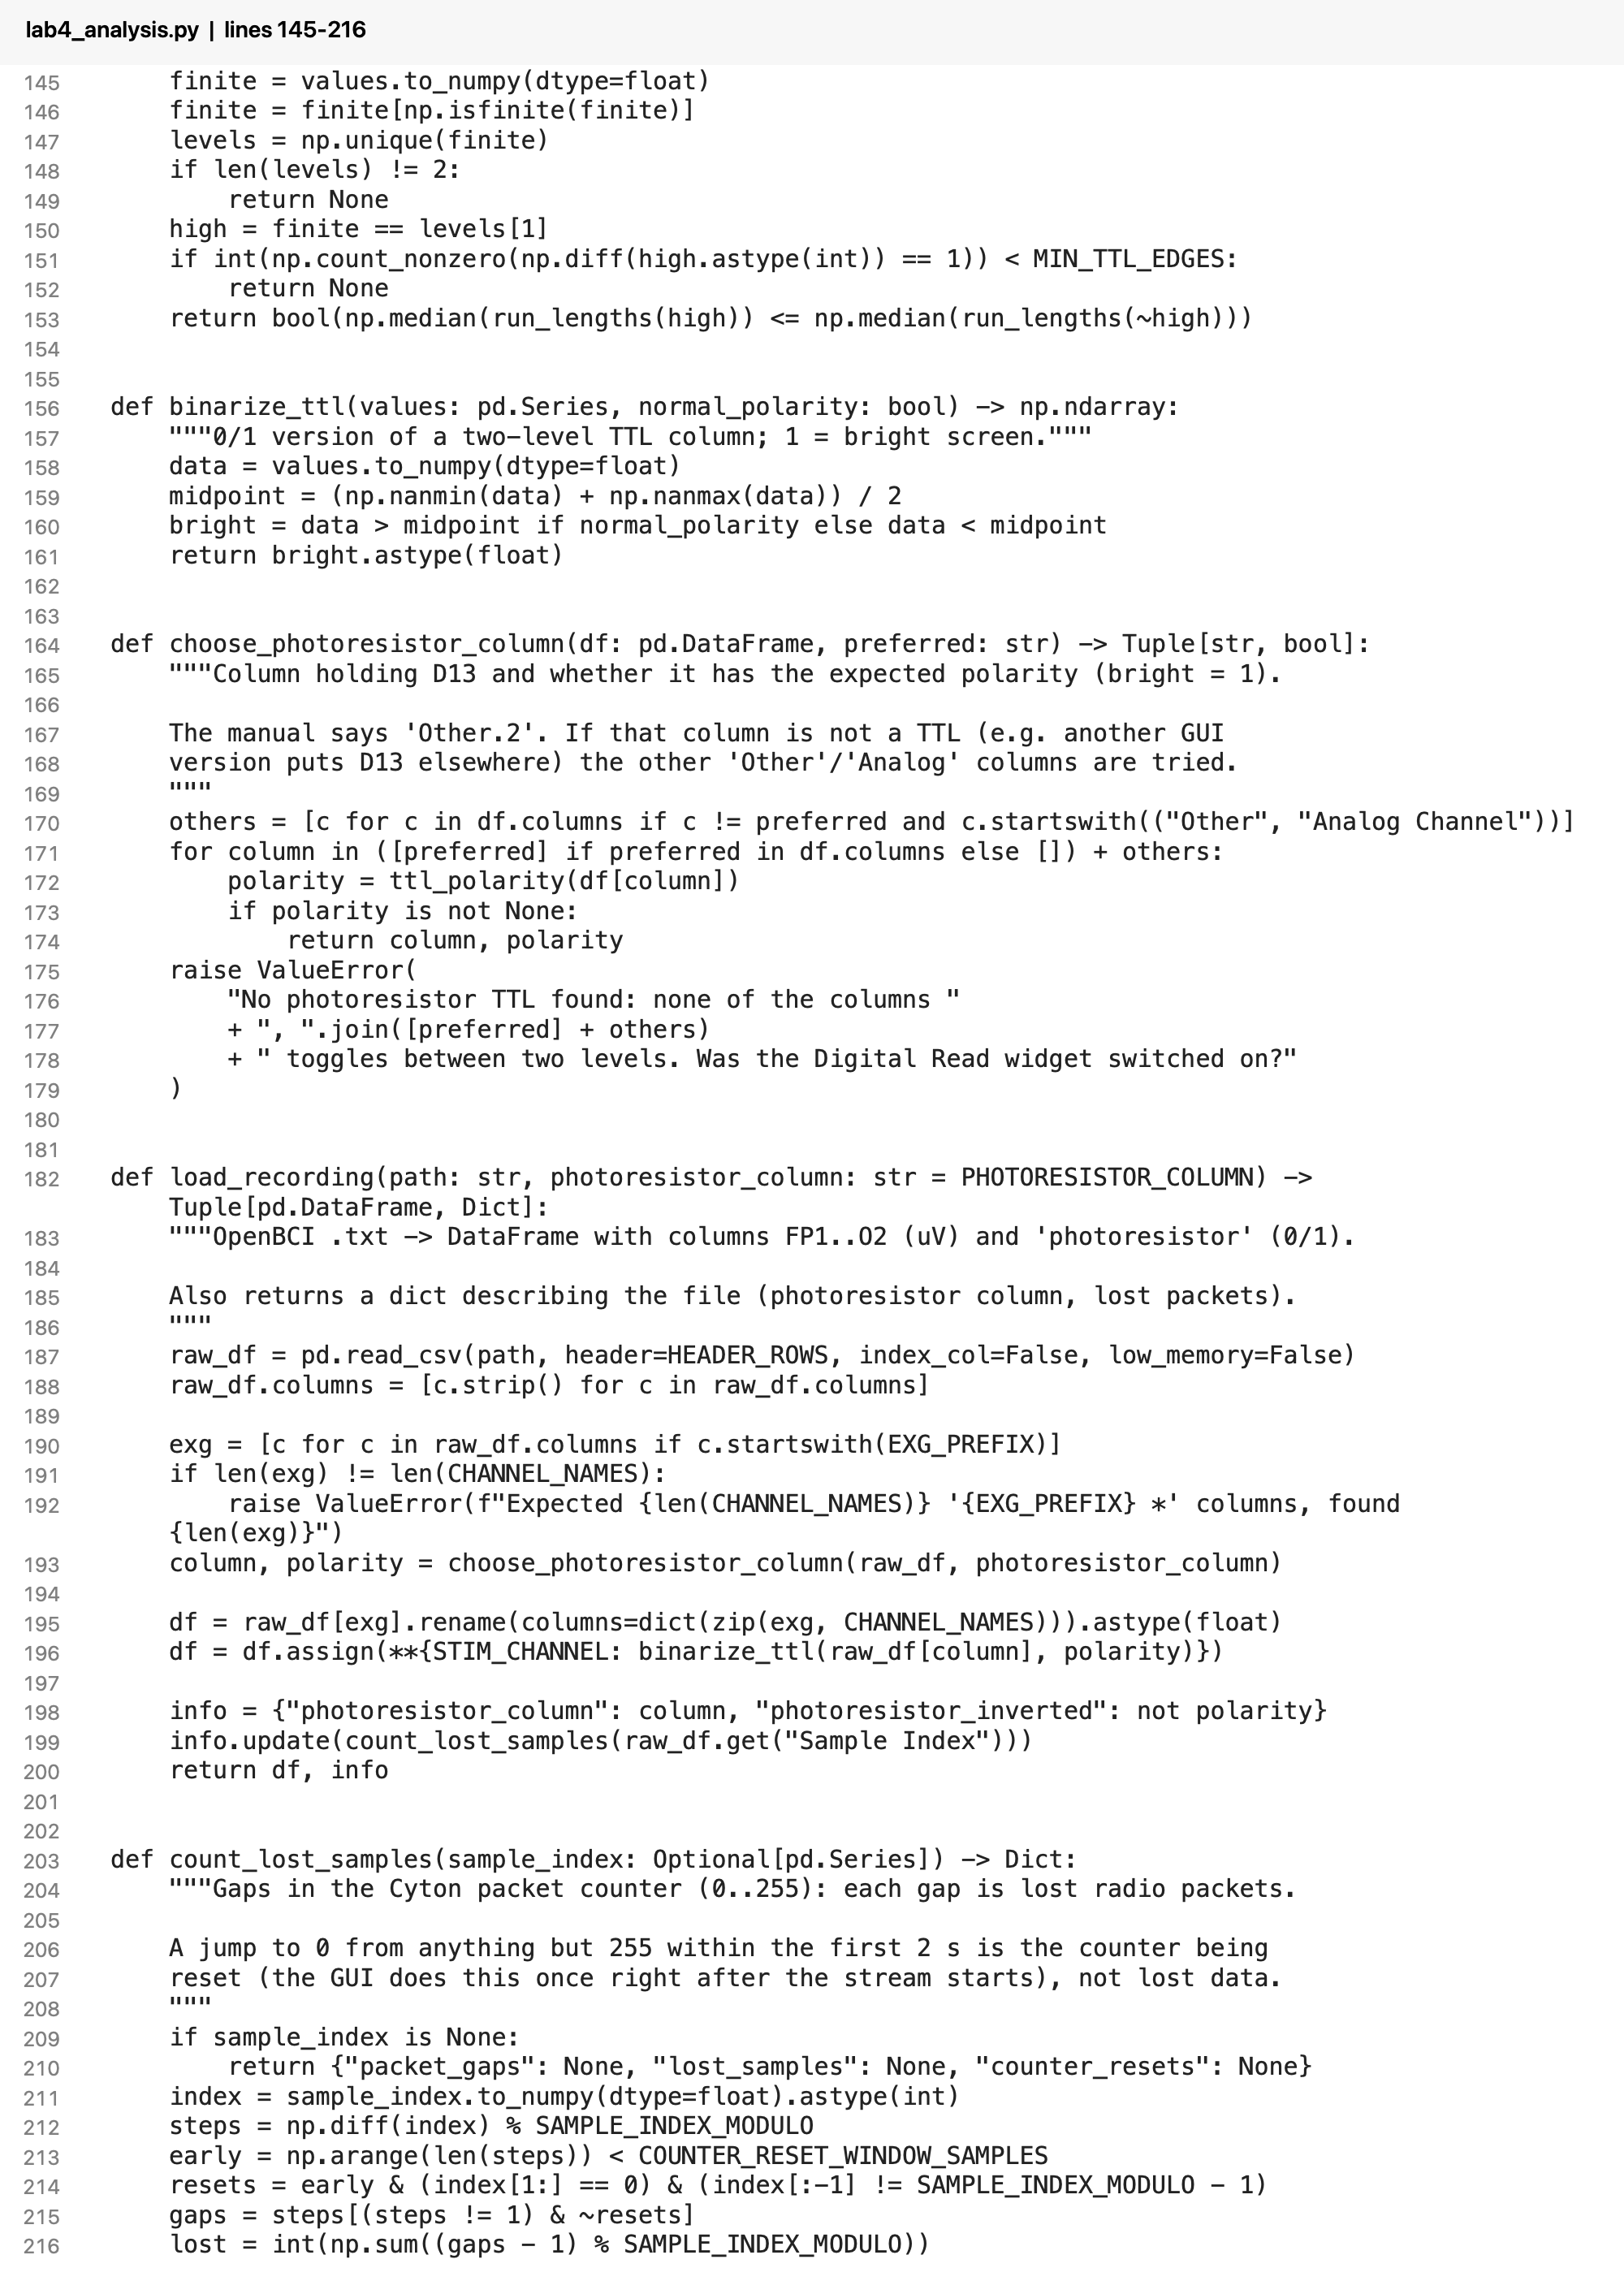
\includegraphics[width=\linewidth,height=0.92\textheight,keepaspectratio]{code_screenshots/analysis-03.png}
  \caption{\texttt{lab4\_analysis.py}, lines 145--216.}
\end{figure}
\clearpage
\begin{figure}[H]
  \centering
  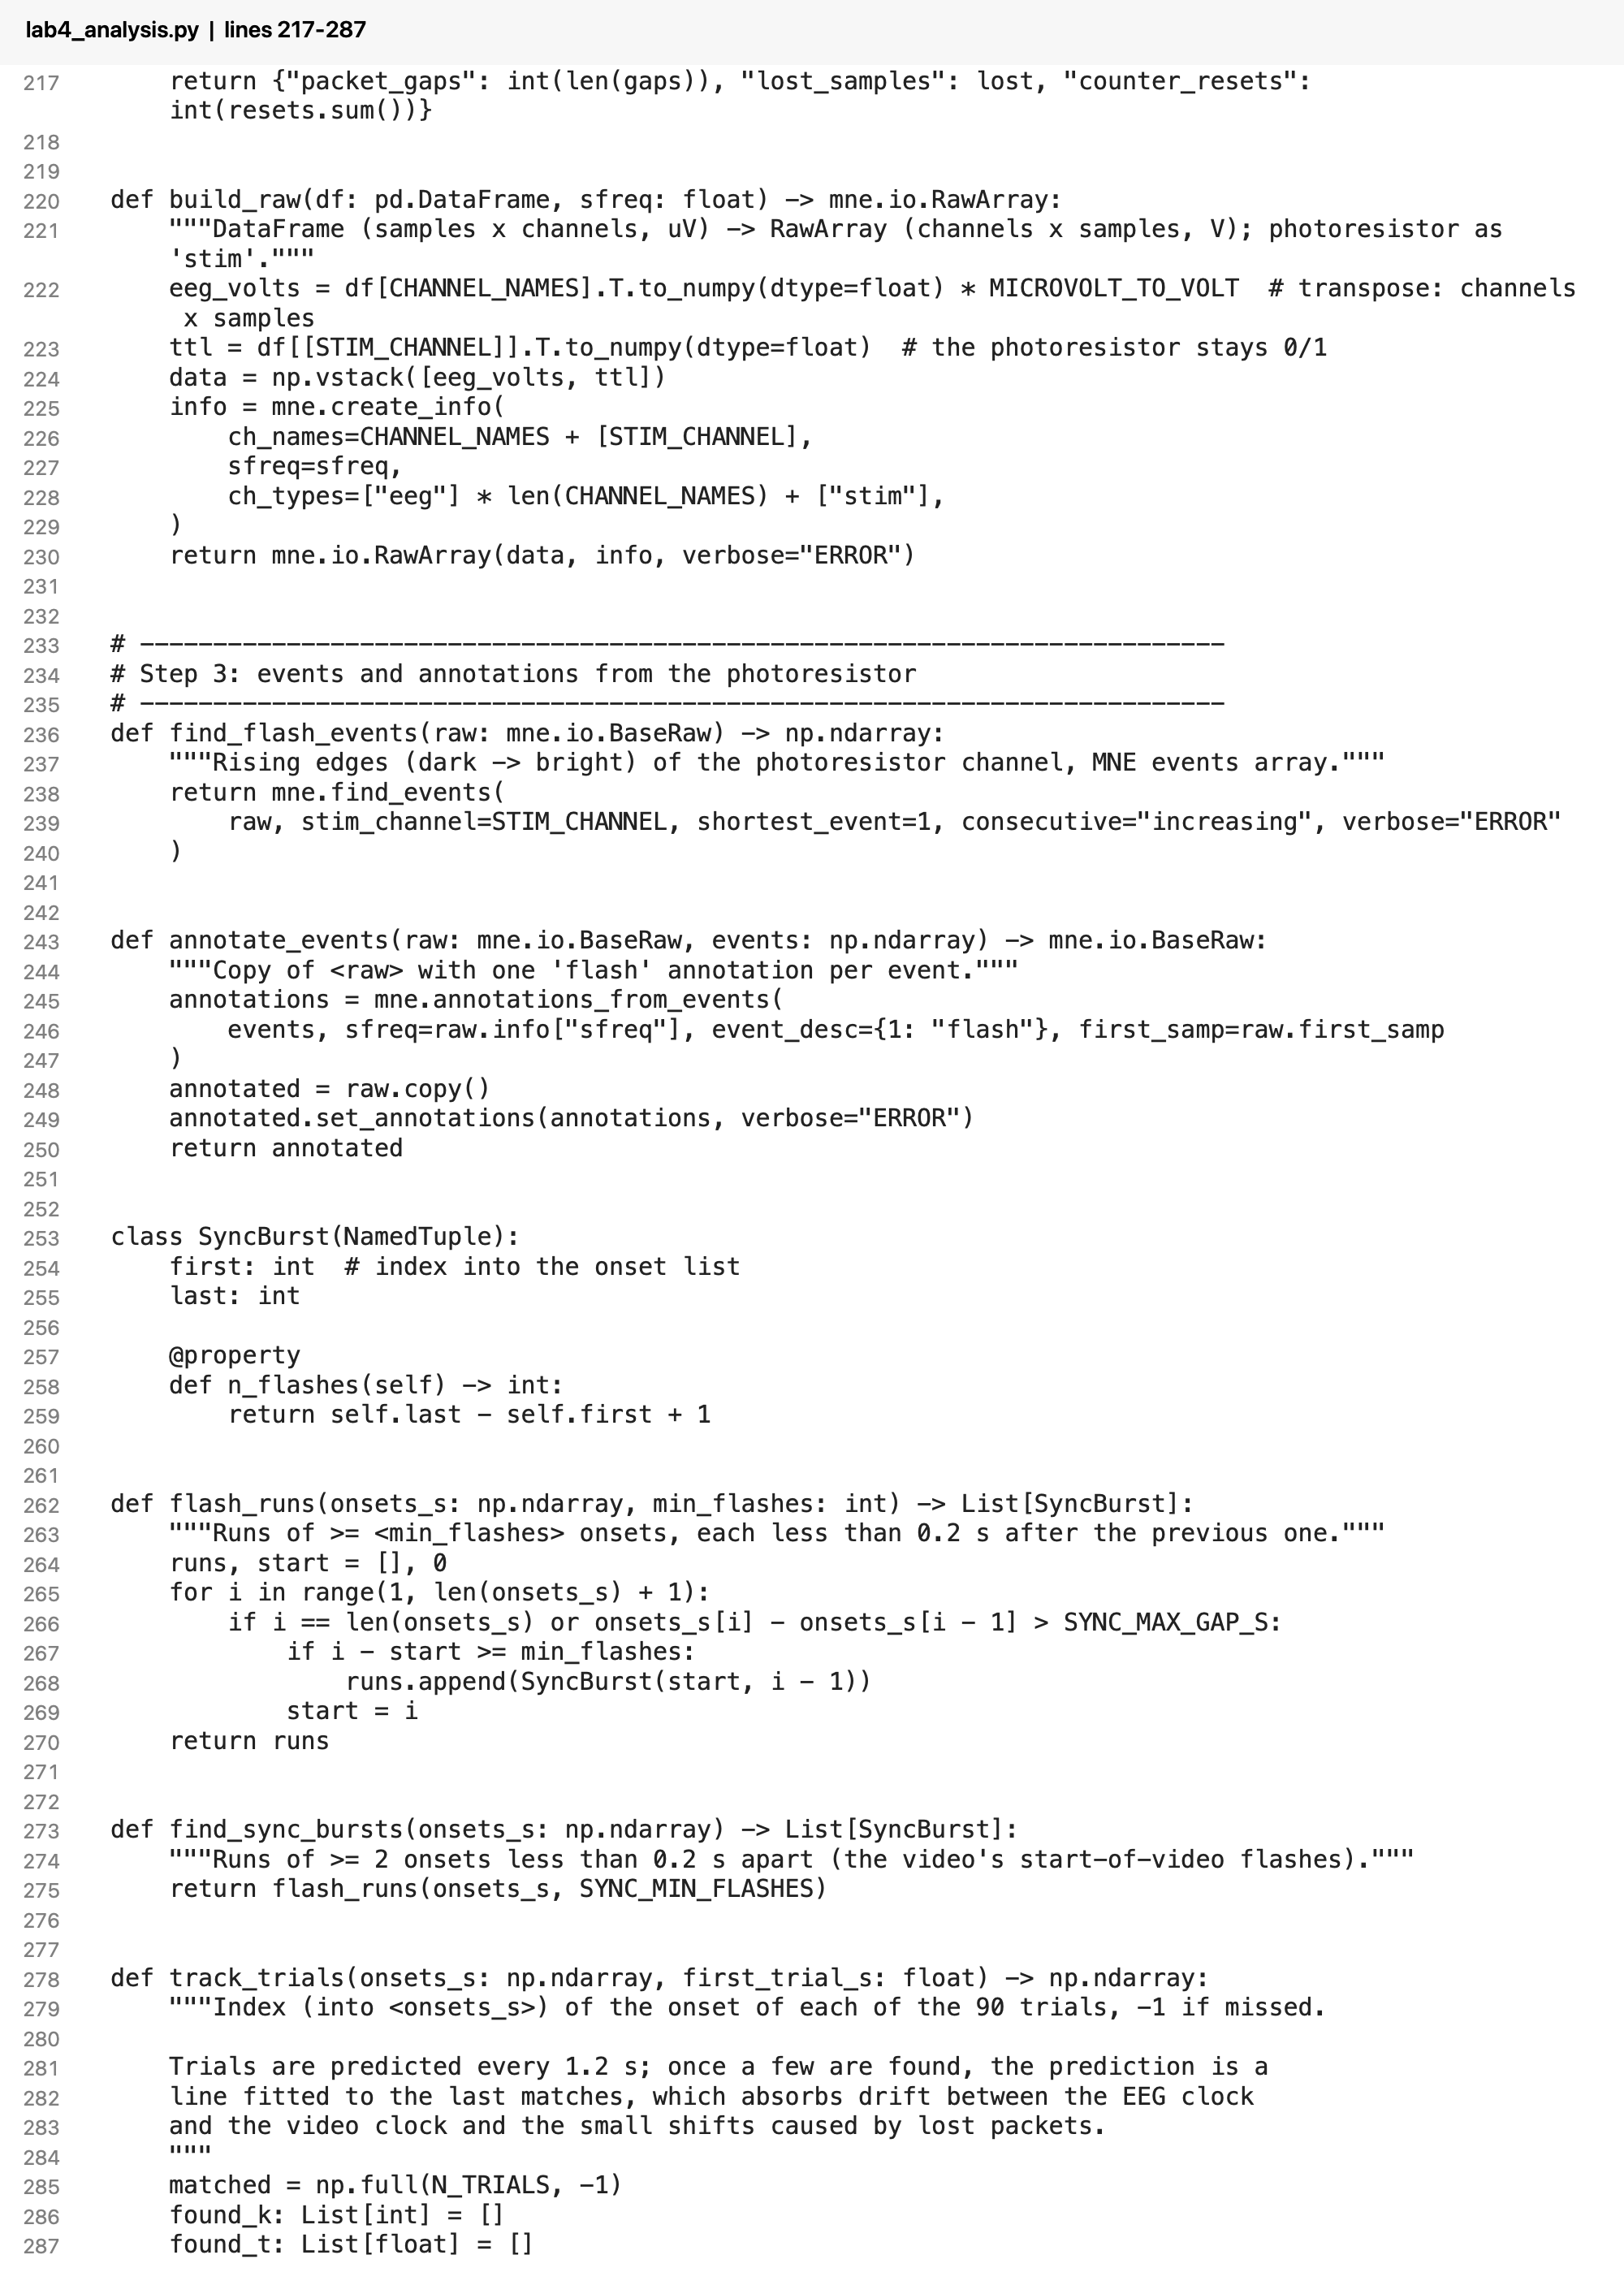
\includegraphics[width=\linewidth,height=0.92\textheight,keepaspectratio]{code_screenshots/analysis-04.png}
  \caption{\texttt{lab4\_analysis.py}, lines 217--287.}
\end{figure}
\clearpage
\begin{figure}[H]
  \centering
  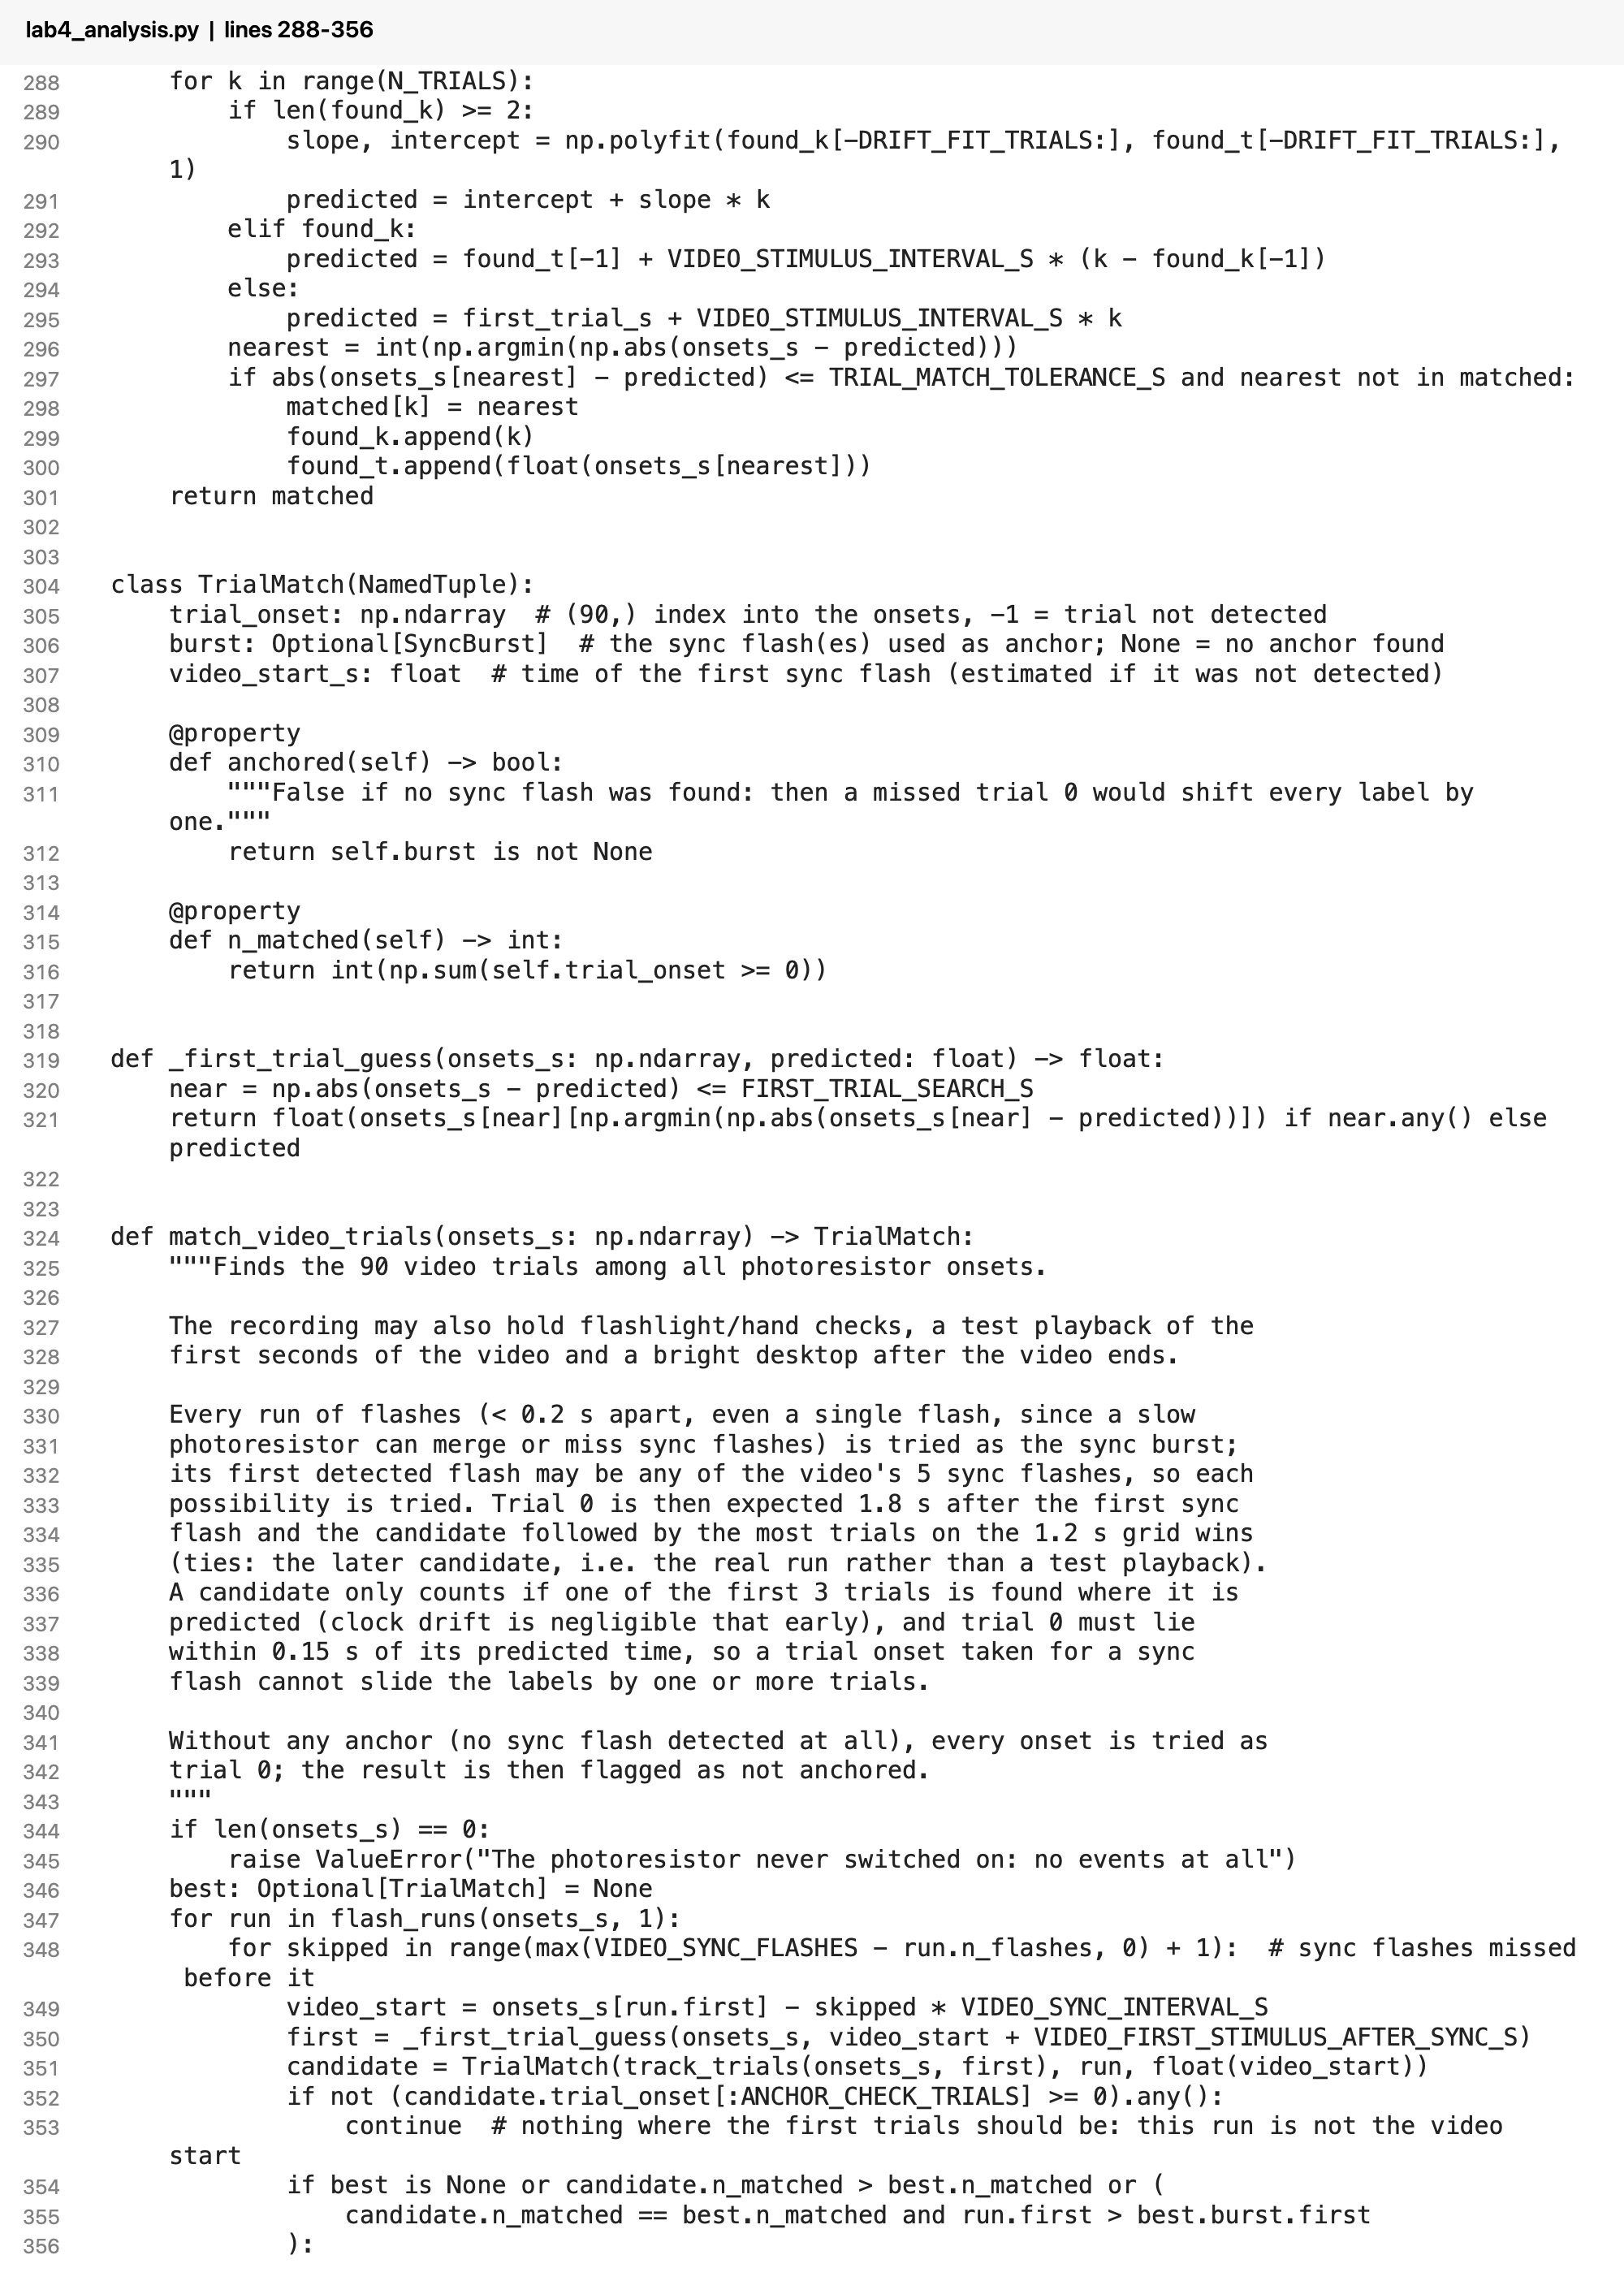
\includegraphics[width=\linewidth,height=0.92\textheight,keepaspectratio]{code_screenshots/analysis-05.png}
  \caption{\texttt{lab4\_analysis.py}, lines 288--356.}
\end{figure}
\clearpage
\begin{figure}[H]
  \centering
  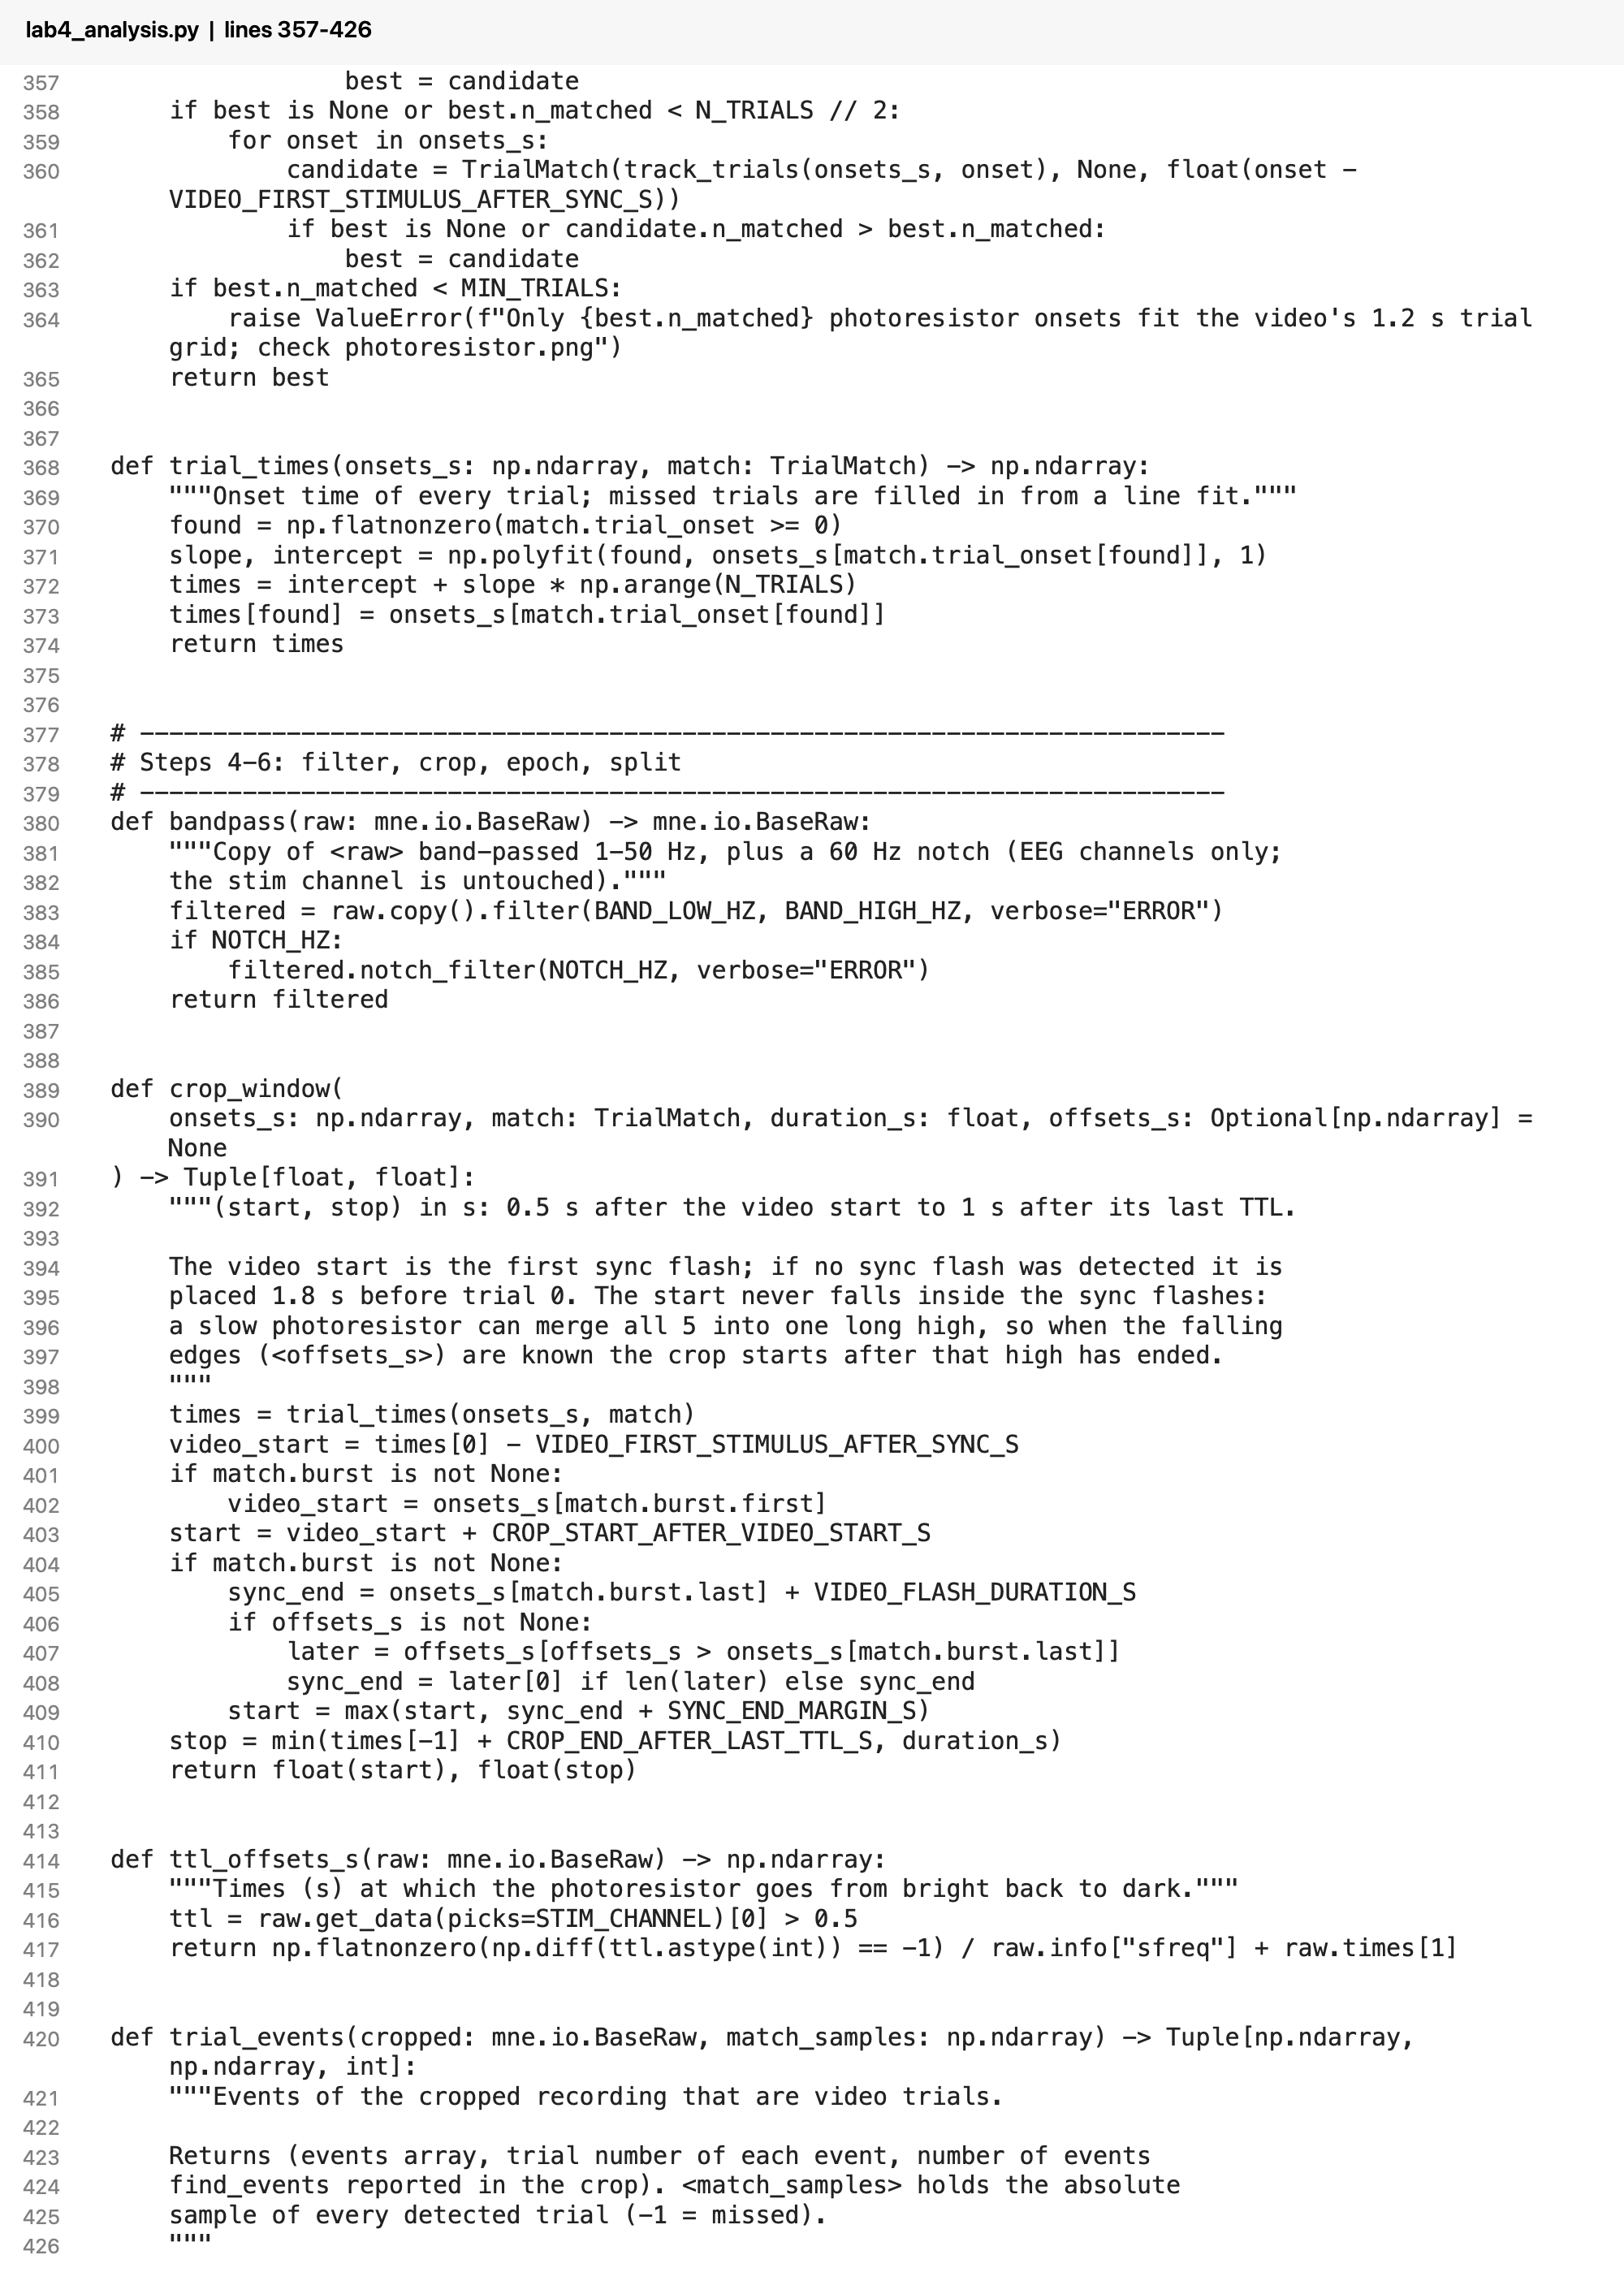
\includegraphics[width=\linewidth,height=0.92\textheight,keepaspectratio]{code_screenshots/analysis-06.png}
  \caption{\texttt{lab4\_analysis.py}, lines 357--426.}
\end{figure}
\clearpage
\begin{figure}[H]
  \centering
  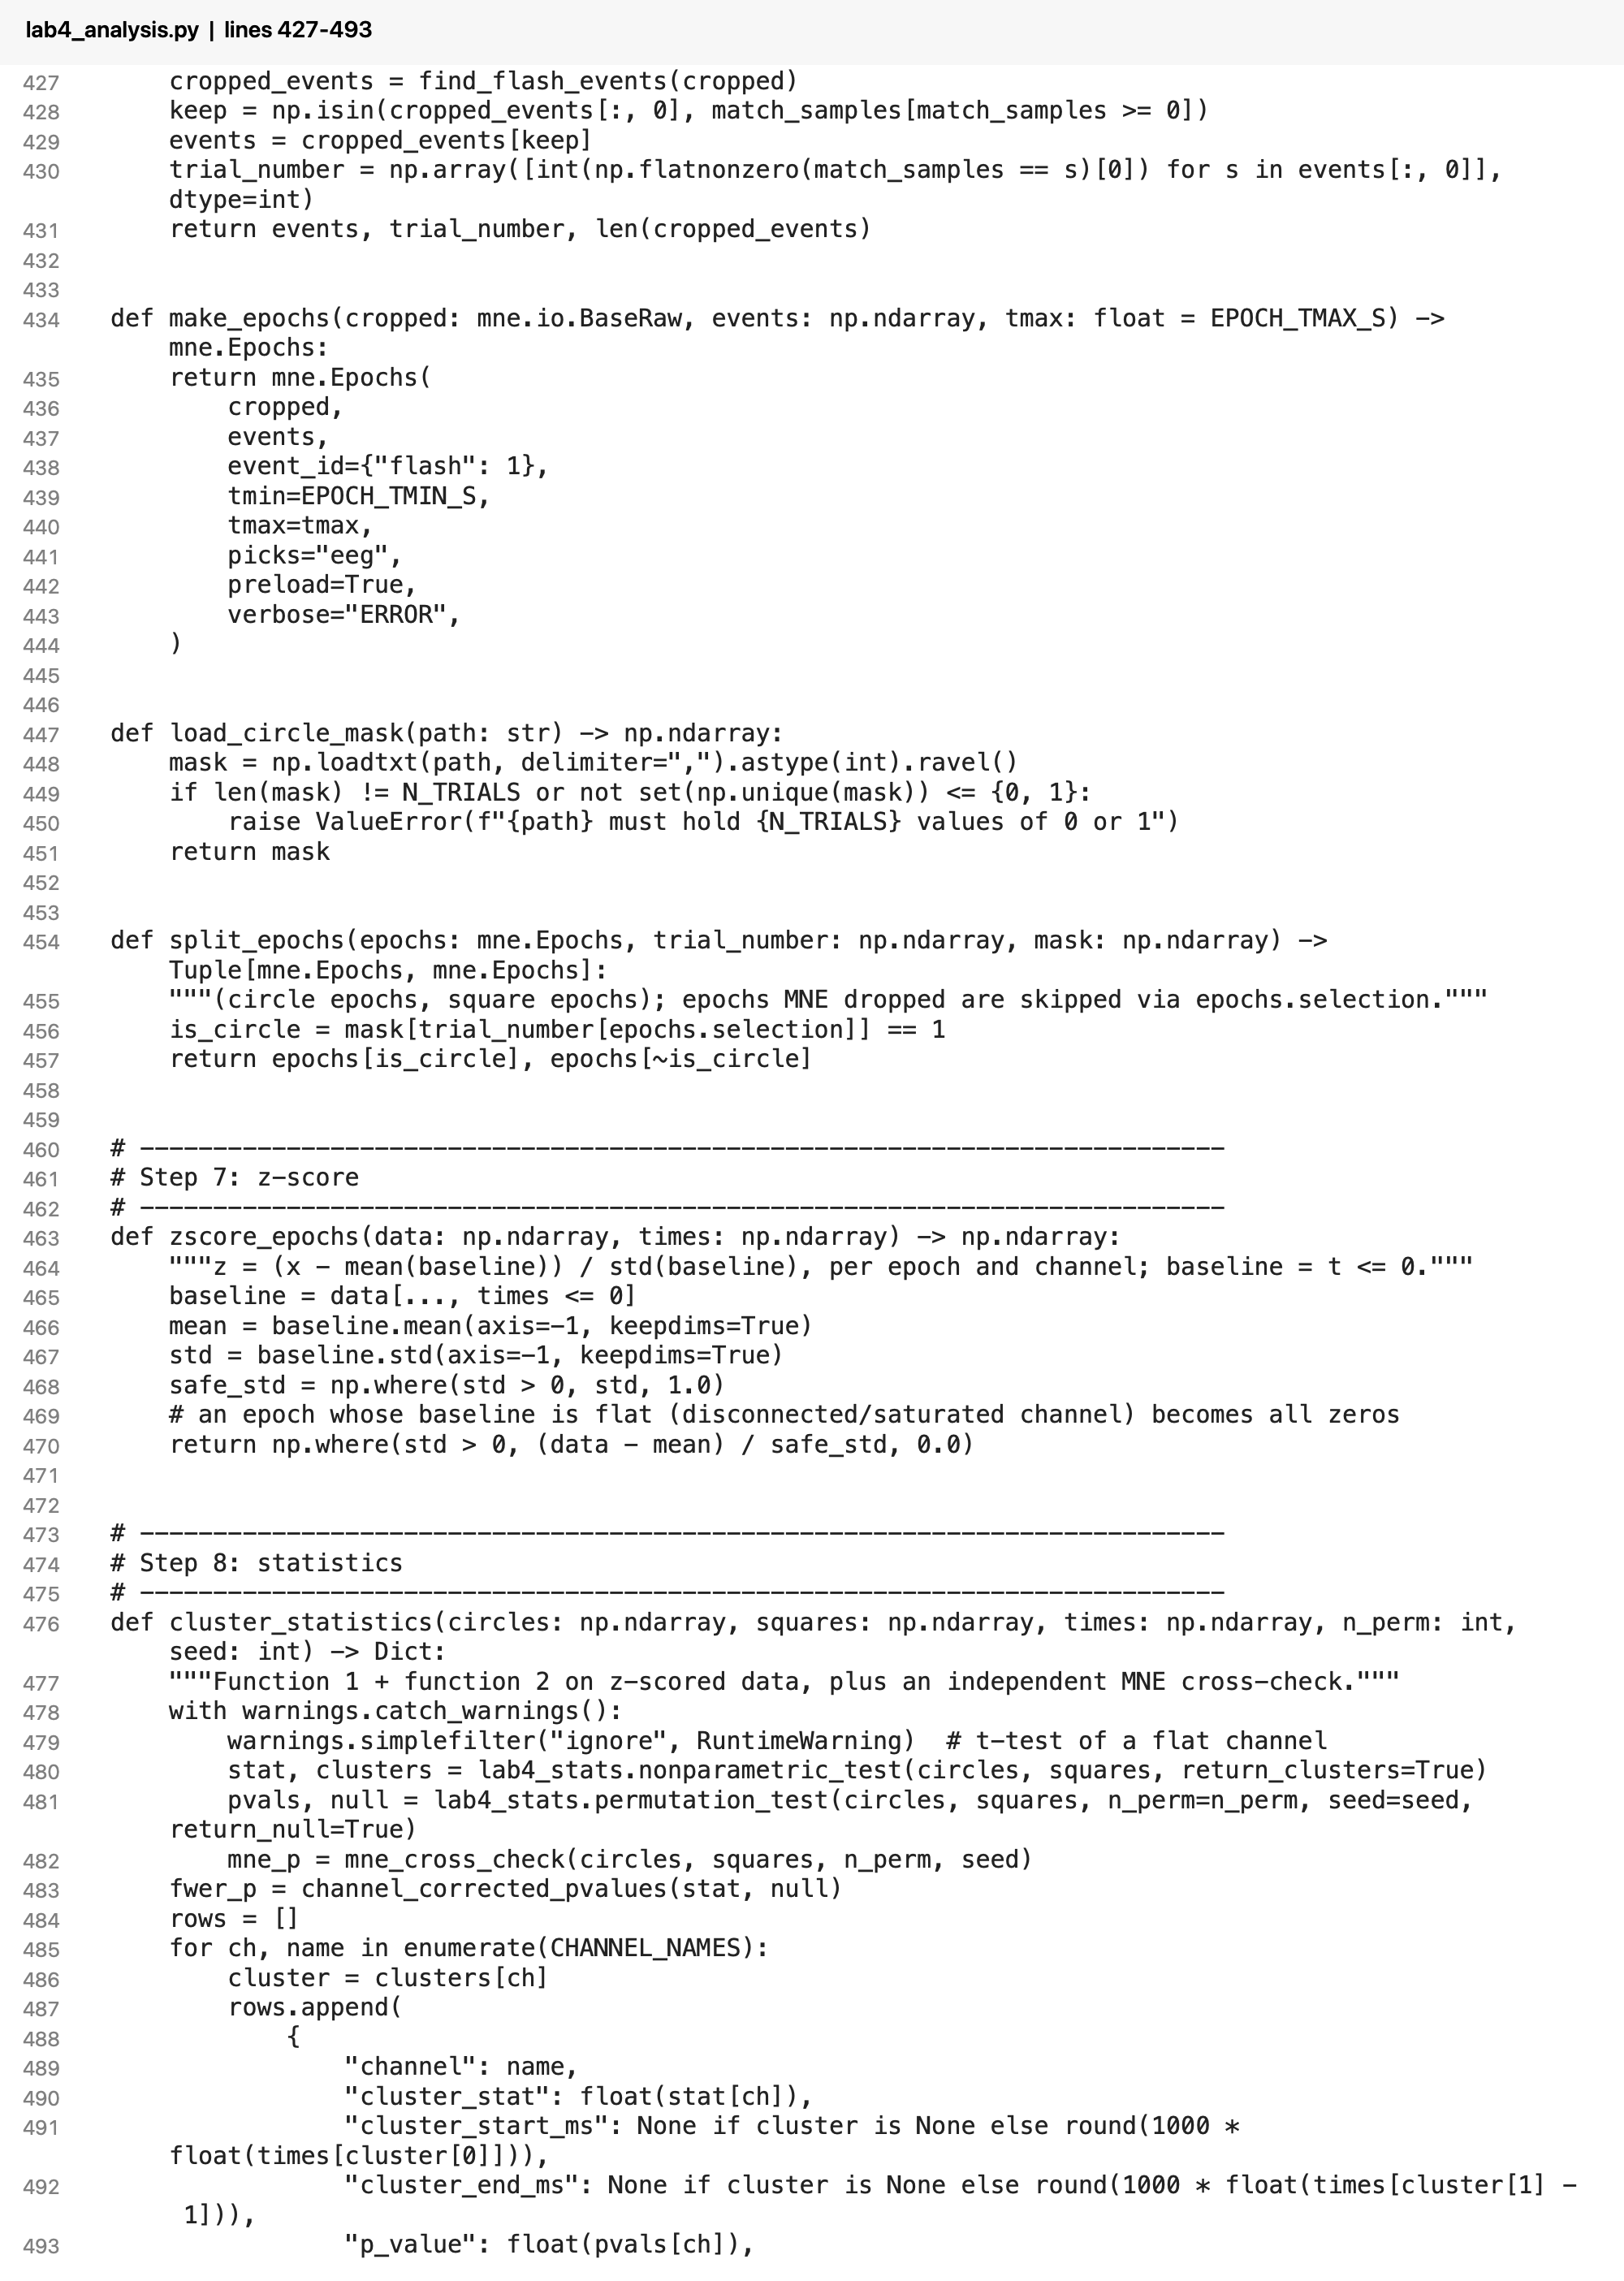
\includegraphics[width=\linewidth,height=0.92\textheight,keepaspectratio]{code_screenshots/analysis-07.png}
  \caption{\texttt{lab4\_analysis.py}, lines 427--493.}
\end{figure}
\clearpage
\begin{figure}[H]
  \centering
  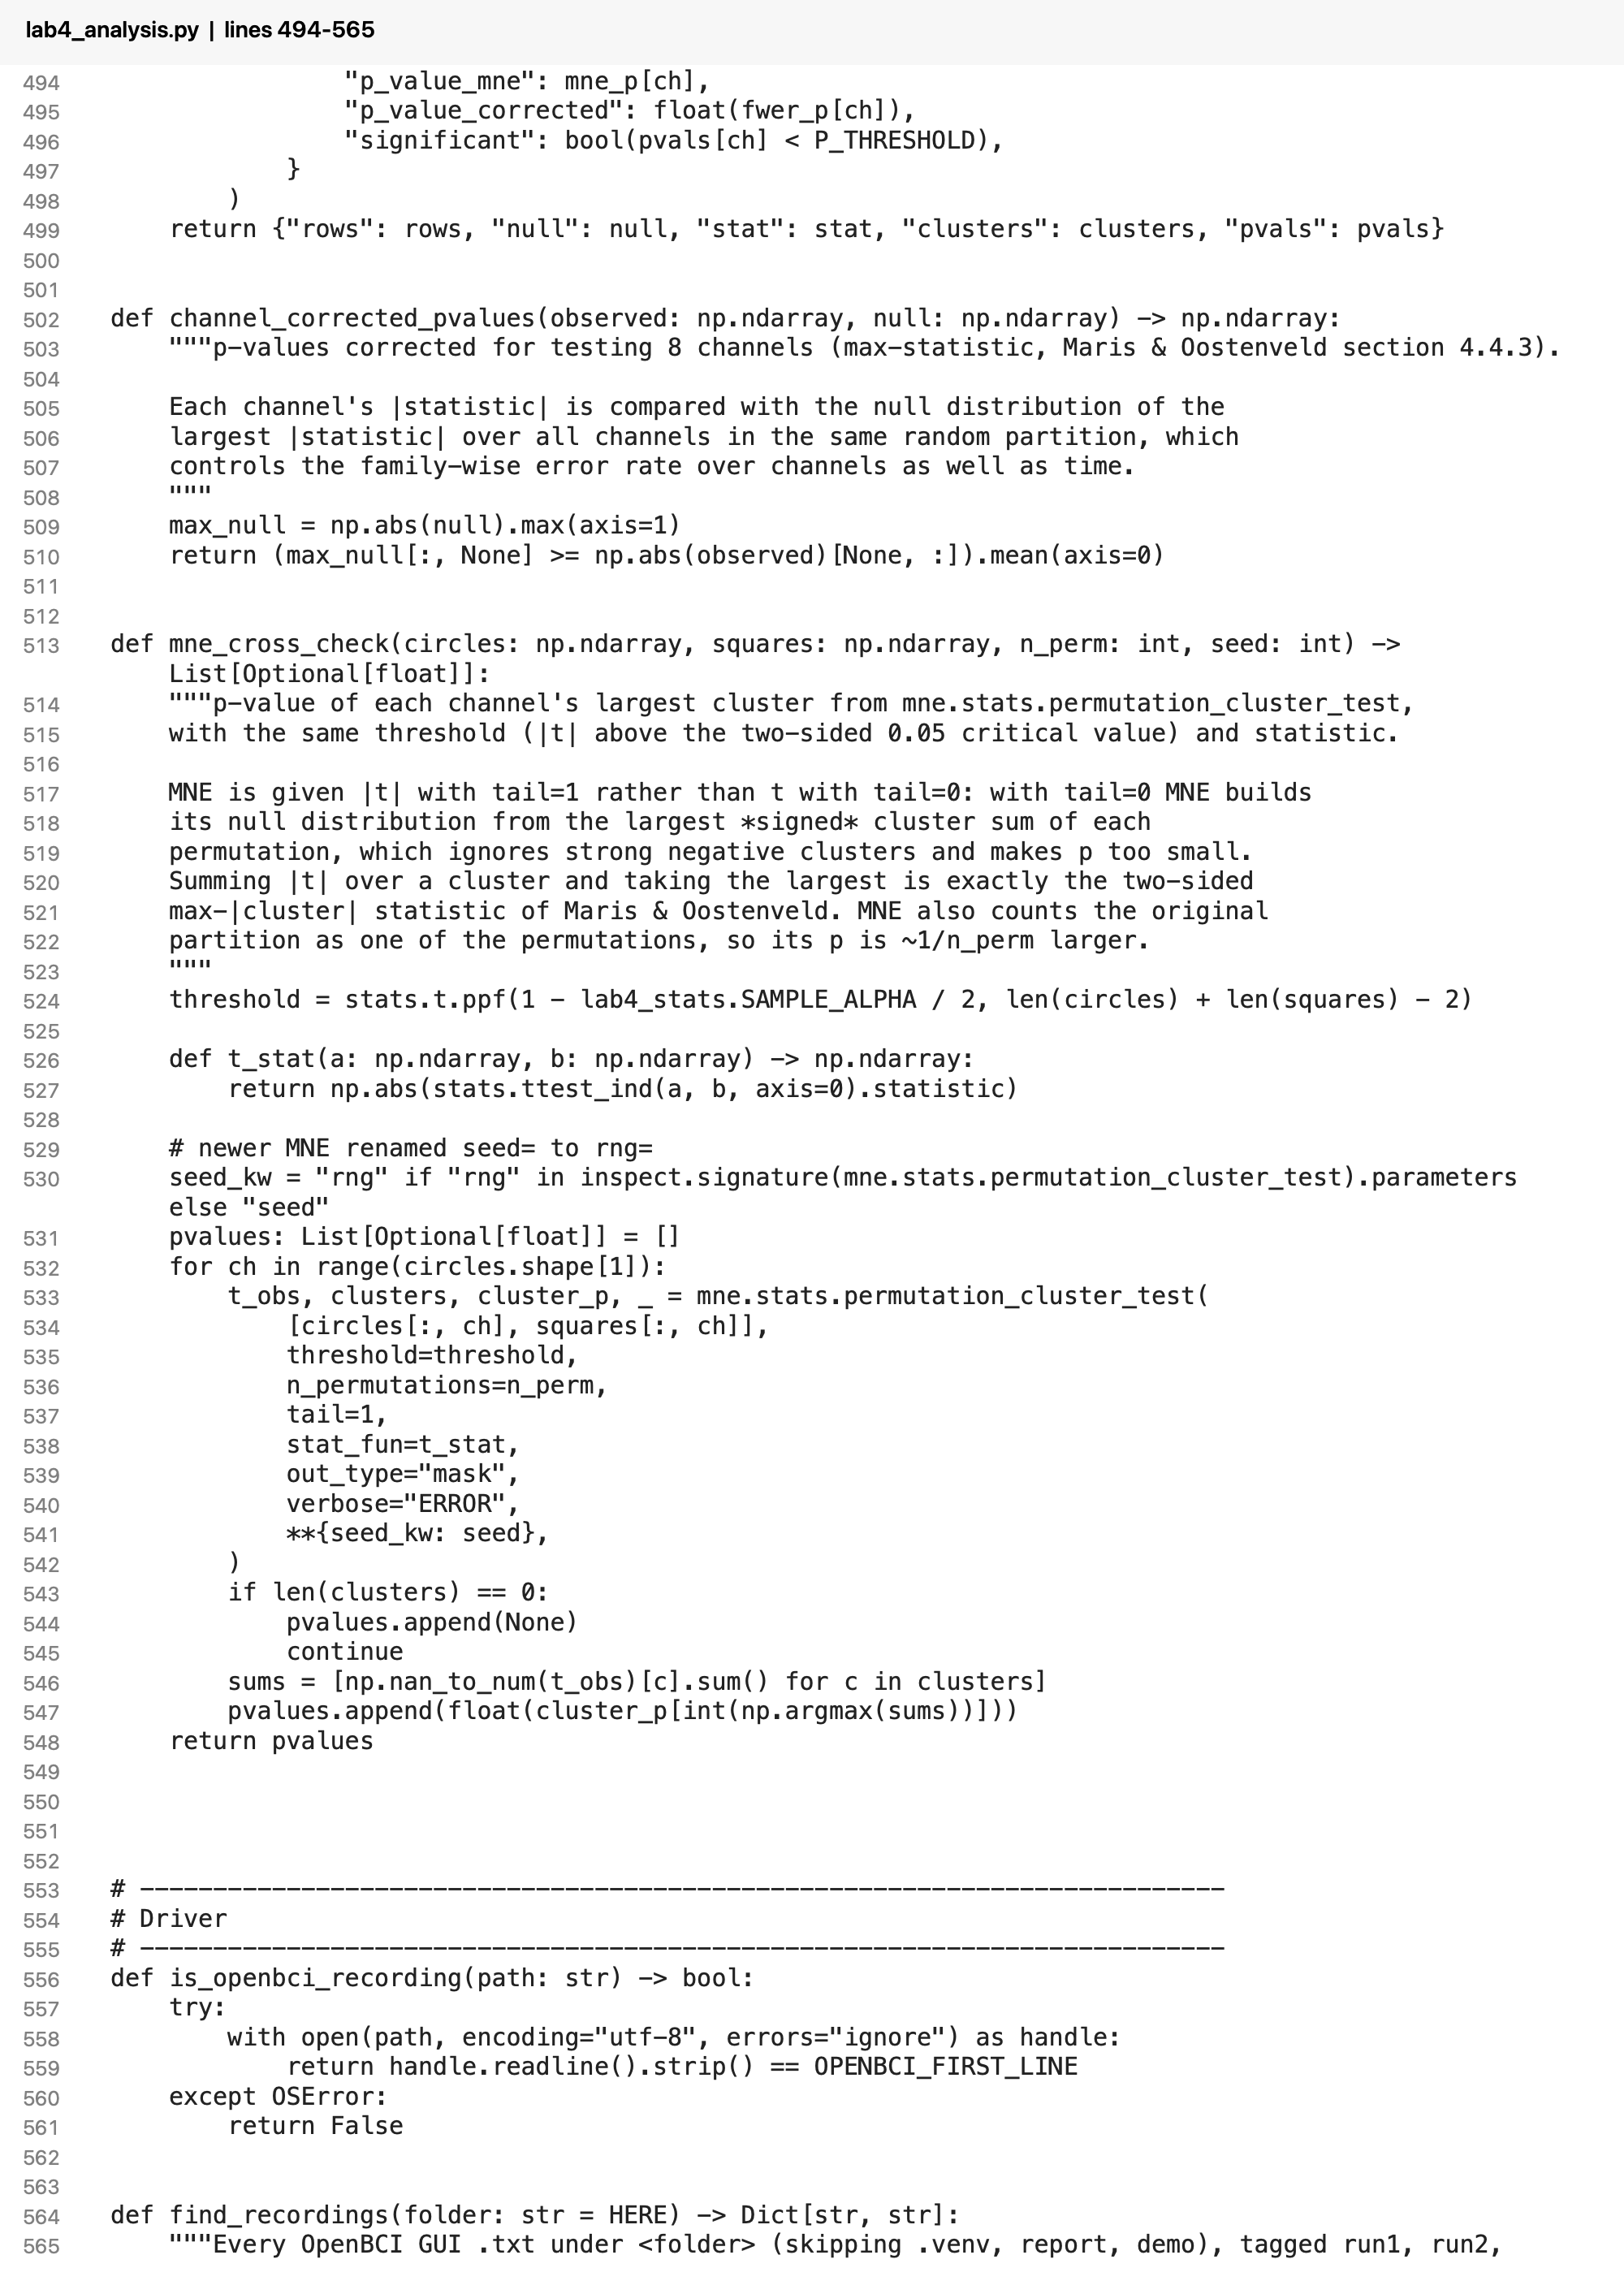
\includegraphics[width=\linewidth,height=0.92\textheight,keepaspectratio]{code_screenshots/analysis-08.png}
  \caption{\texttt{lab4\_analysis.py}, lines 494--565.}
\end{figure}
\clearpage
\begin{figure}[H]
  \centering
  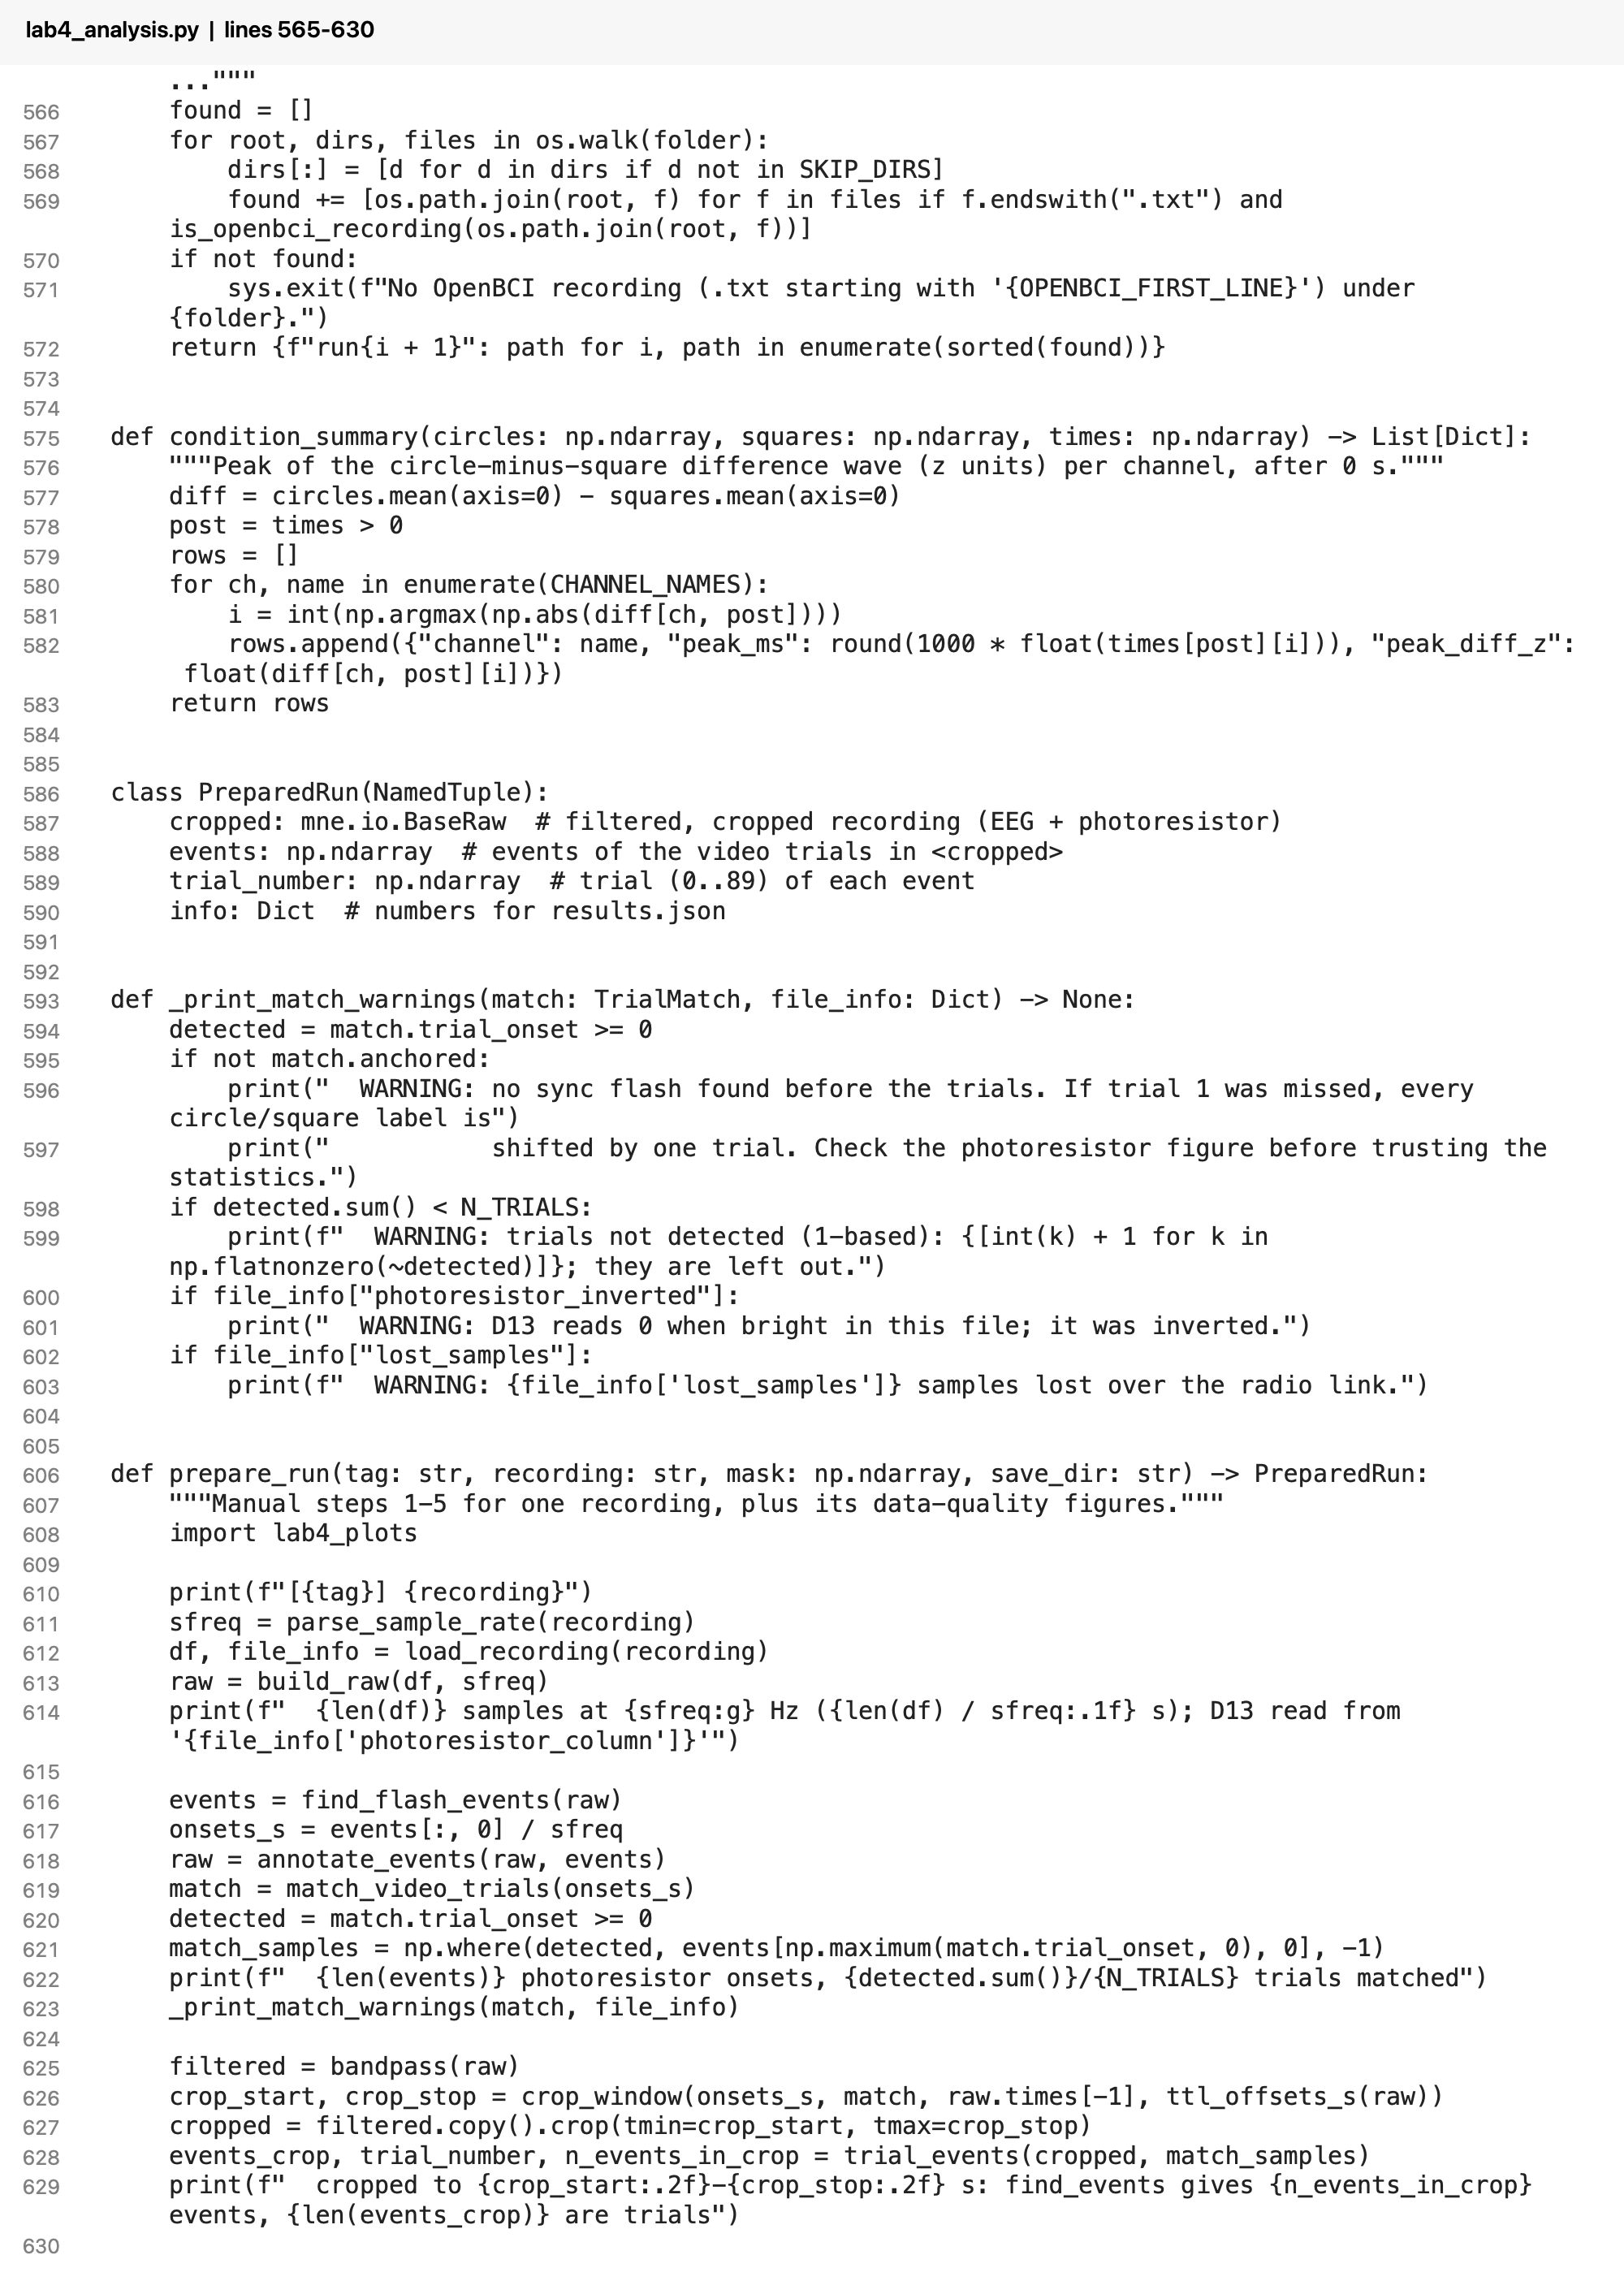
\includegraphics[width=\linewidth,height=0.92\textheight,keepaspectratio]{code_screenshots/analysis-09.png}
  \caption{\texttt{lab4\_analysis.py}, lines 565--630.}
\end{figure}
\clearpage
\begin{figure}[H]
  \centering
  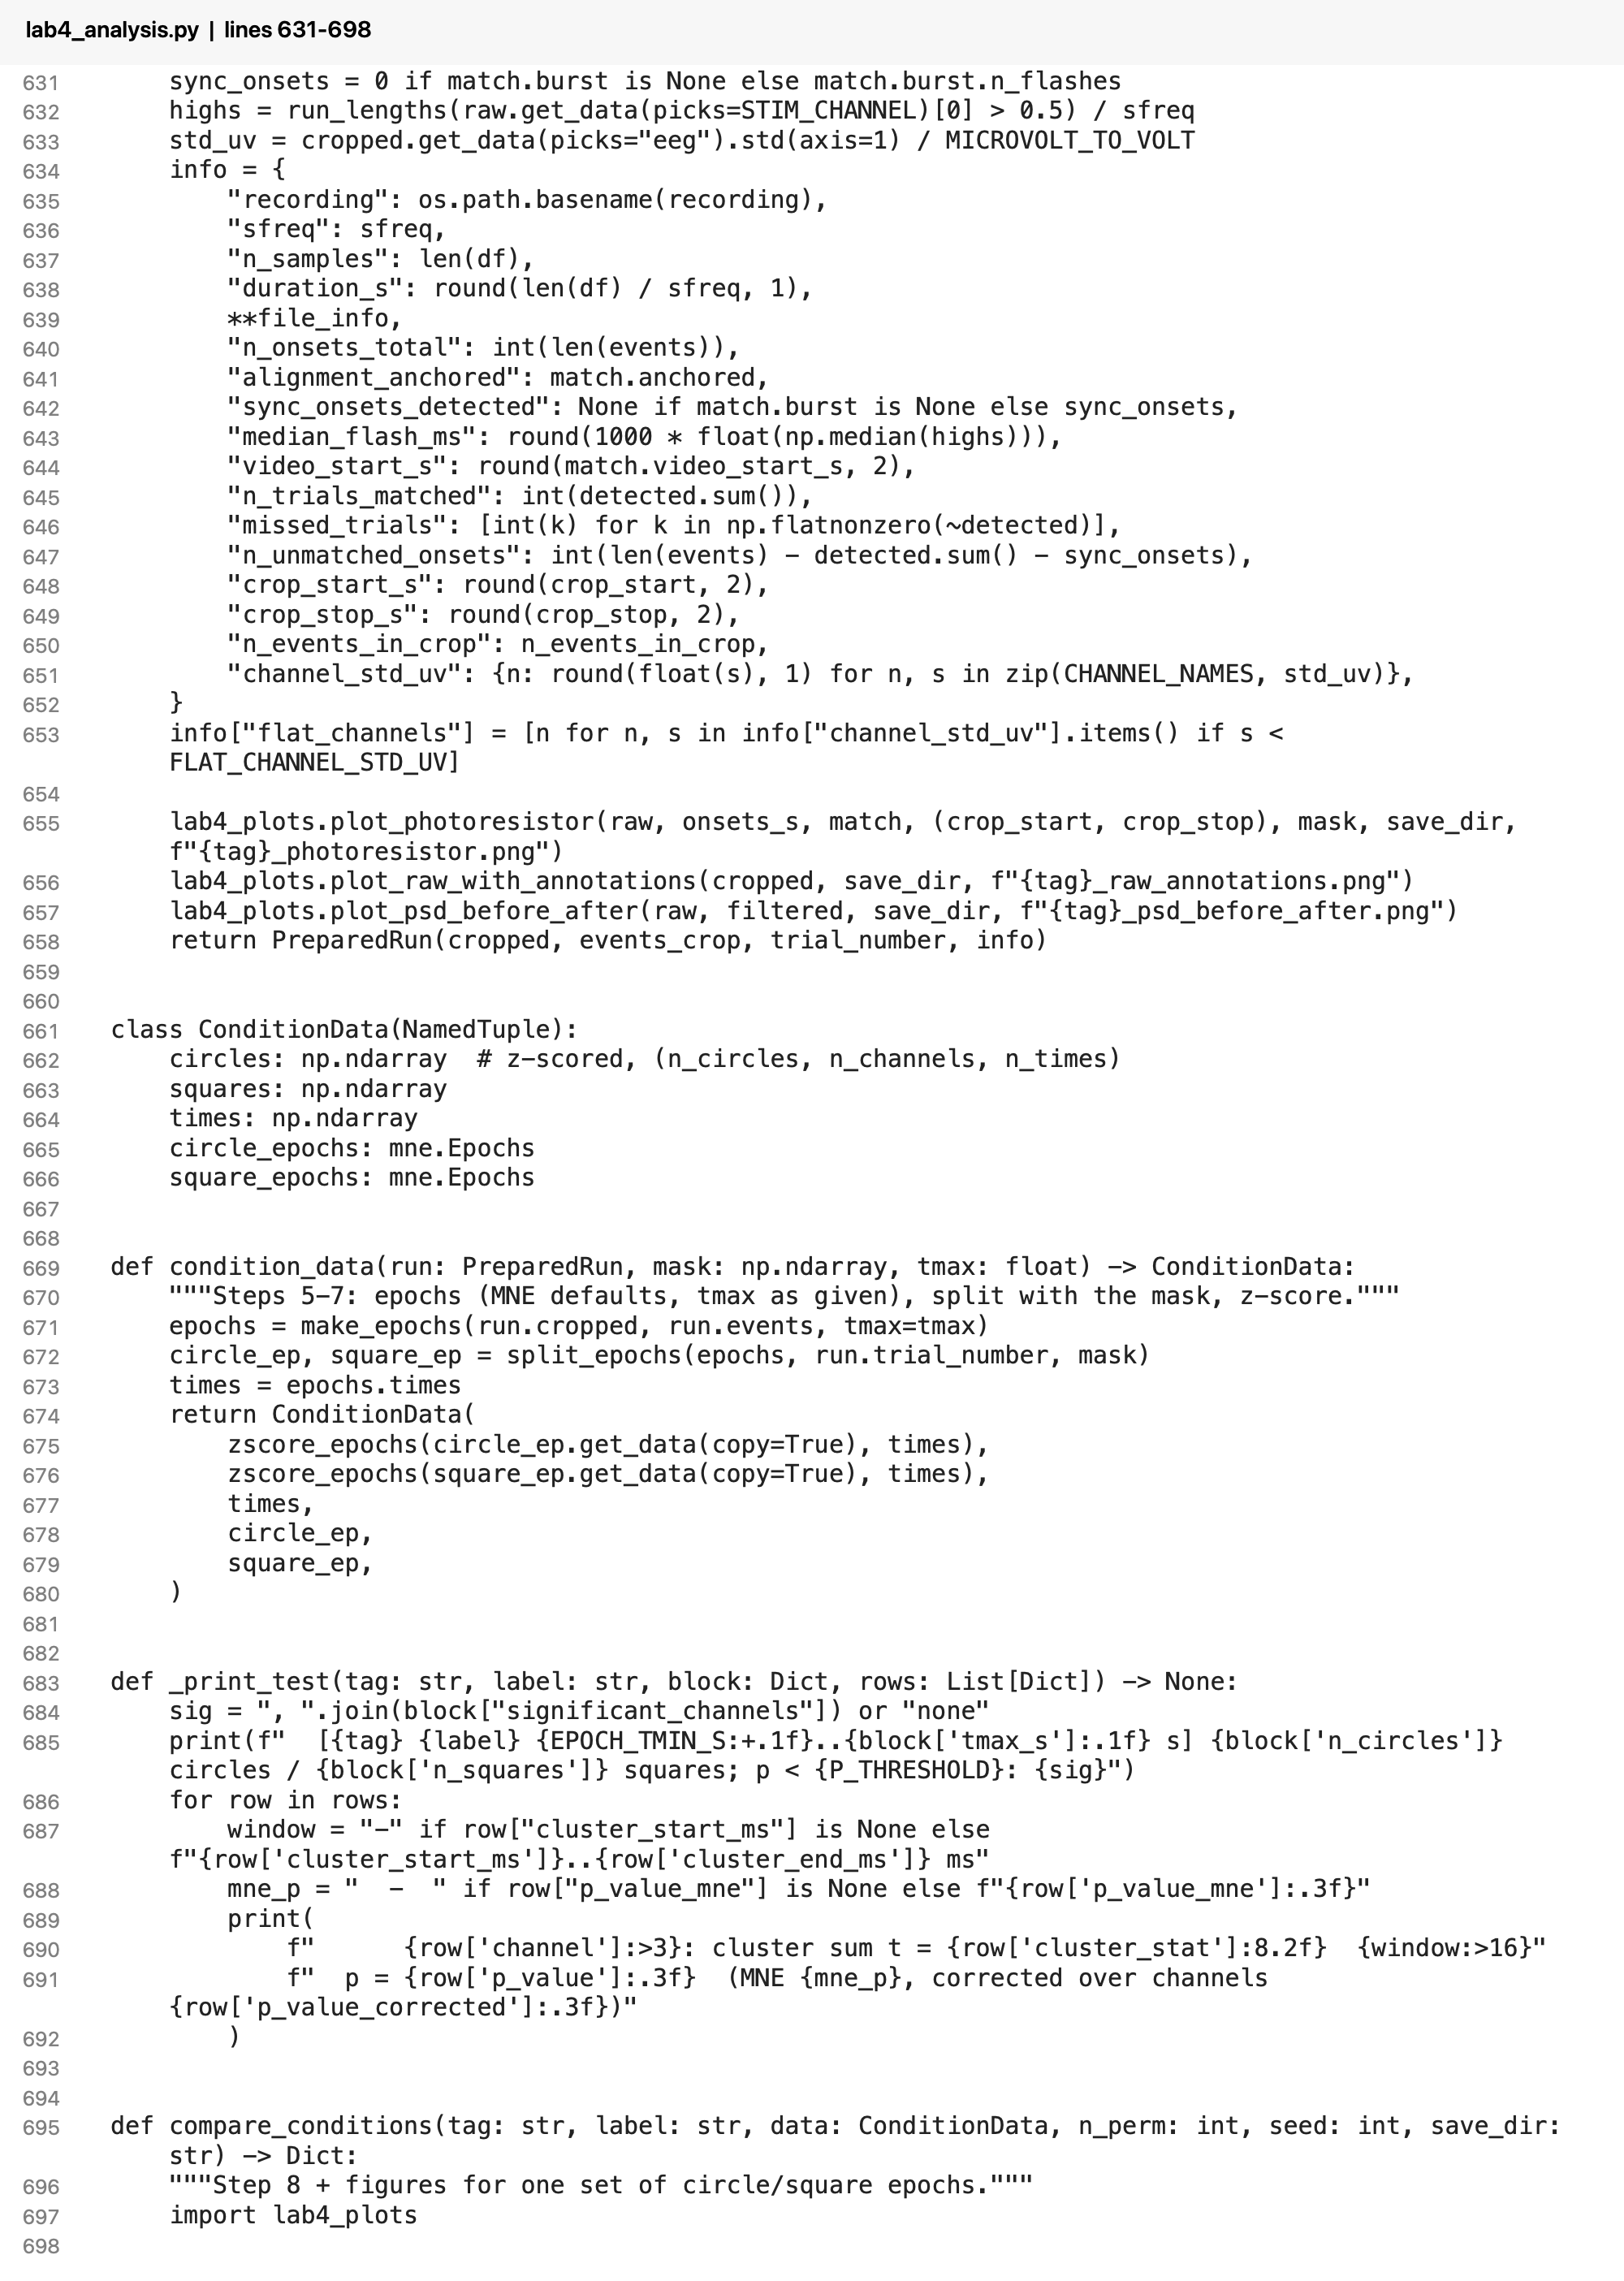
\includegraphics[width=\linewidth,height=0.92\textheight,keepaspectratio]{code_screenshots/analysis-10.png}
  \caption{\texttt{lab4\_analysis.py}, lines 631--698.}
\end{figure}
\clearpage
\begin{figure}[H]
  \centering
  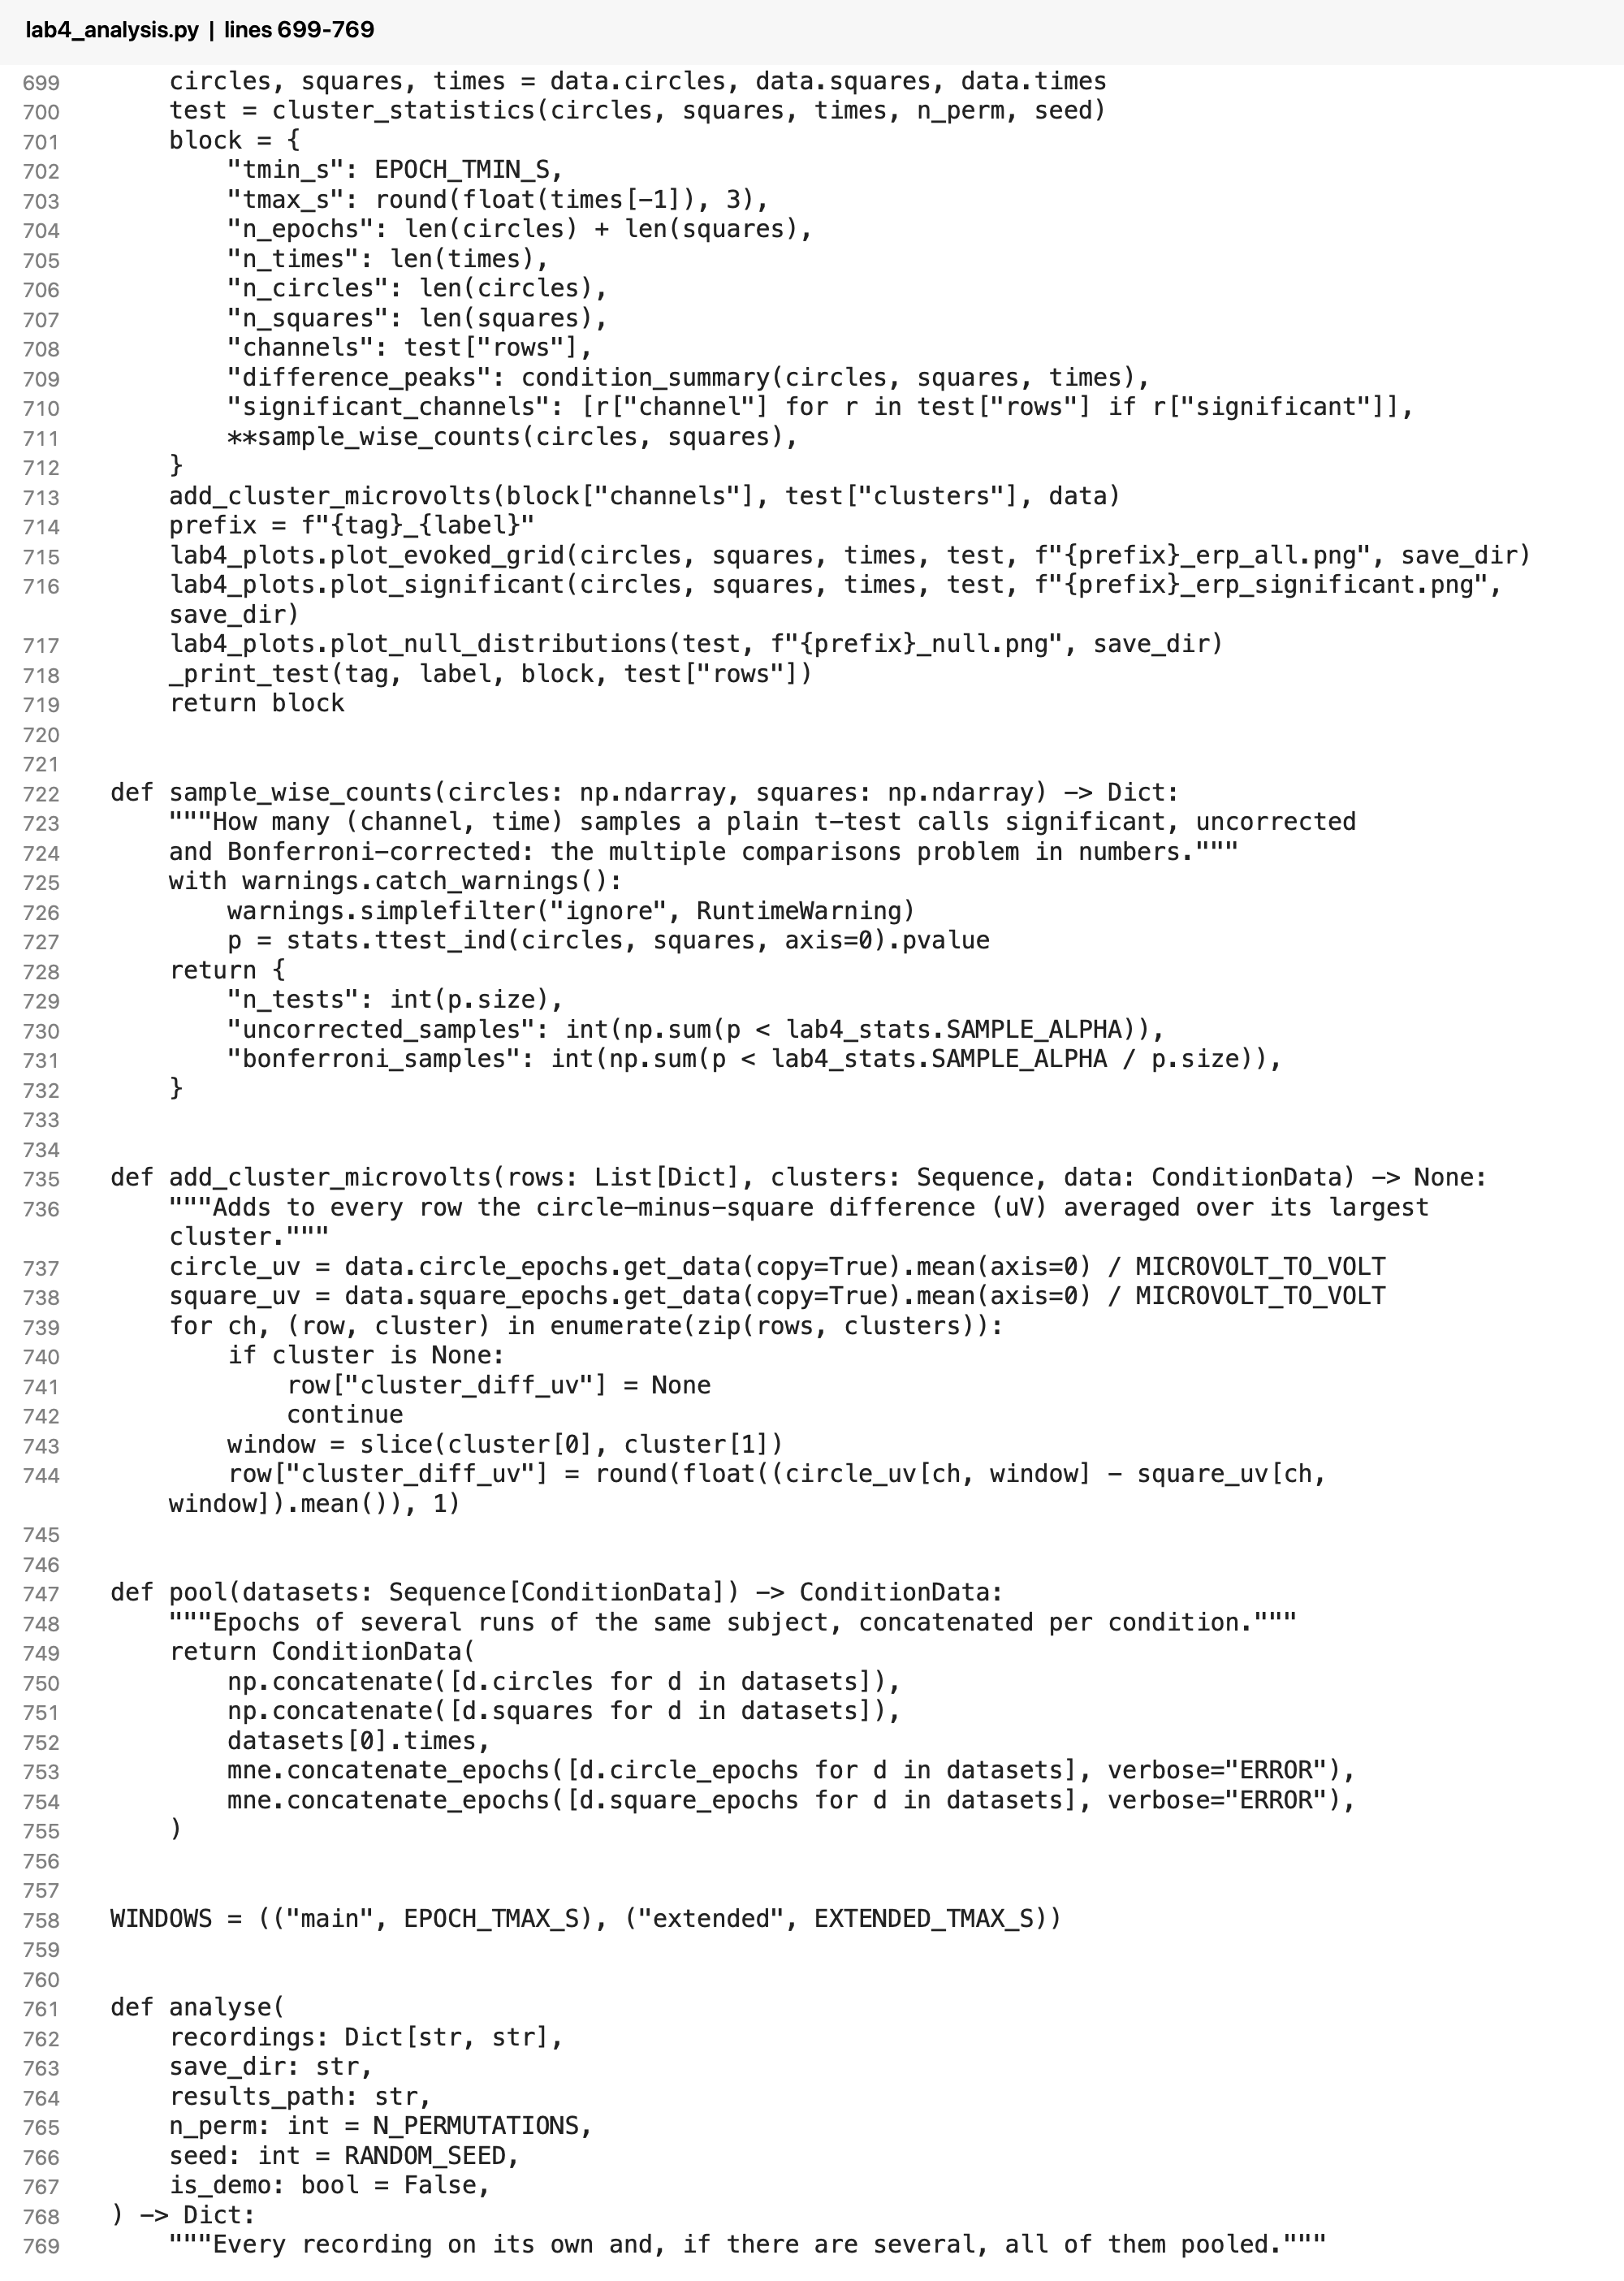
\includegraphics[width=\linewidth,height=0.92\textheight,keepaspectratio]{code_screenshots/analysis-11.png}
  \caption{\texttt{lab4\_analysis.py}, lines 699--769.}
\end{figure}
\clearpage
\begin{figure}[H]
  \centering
  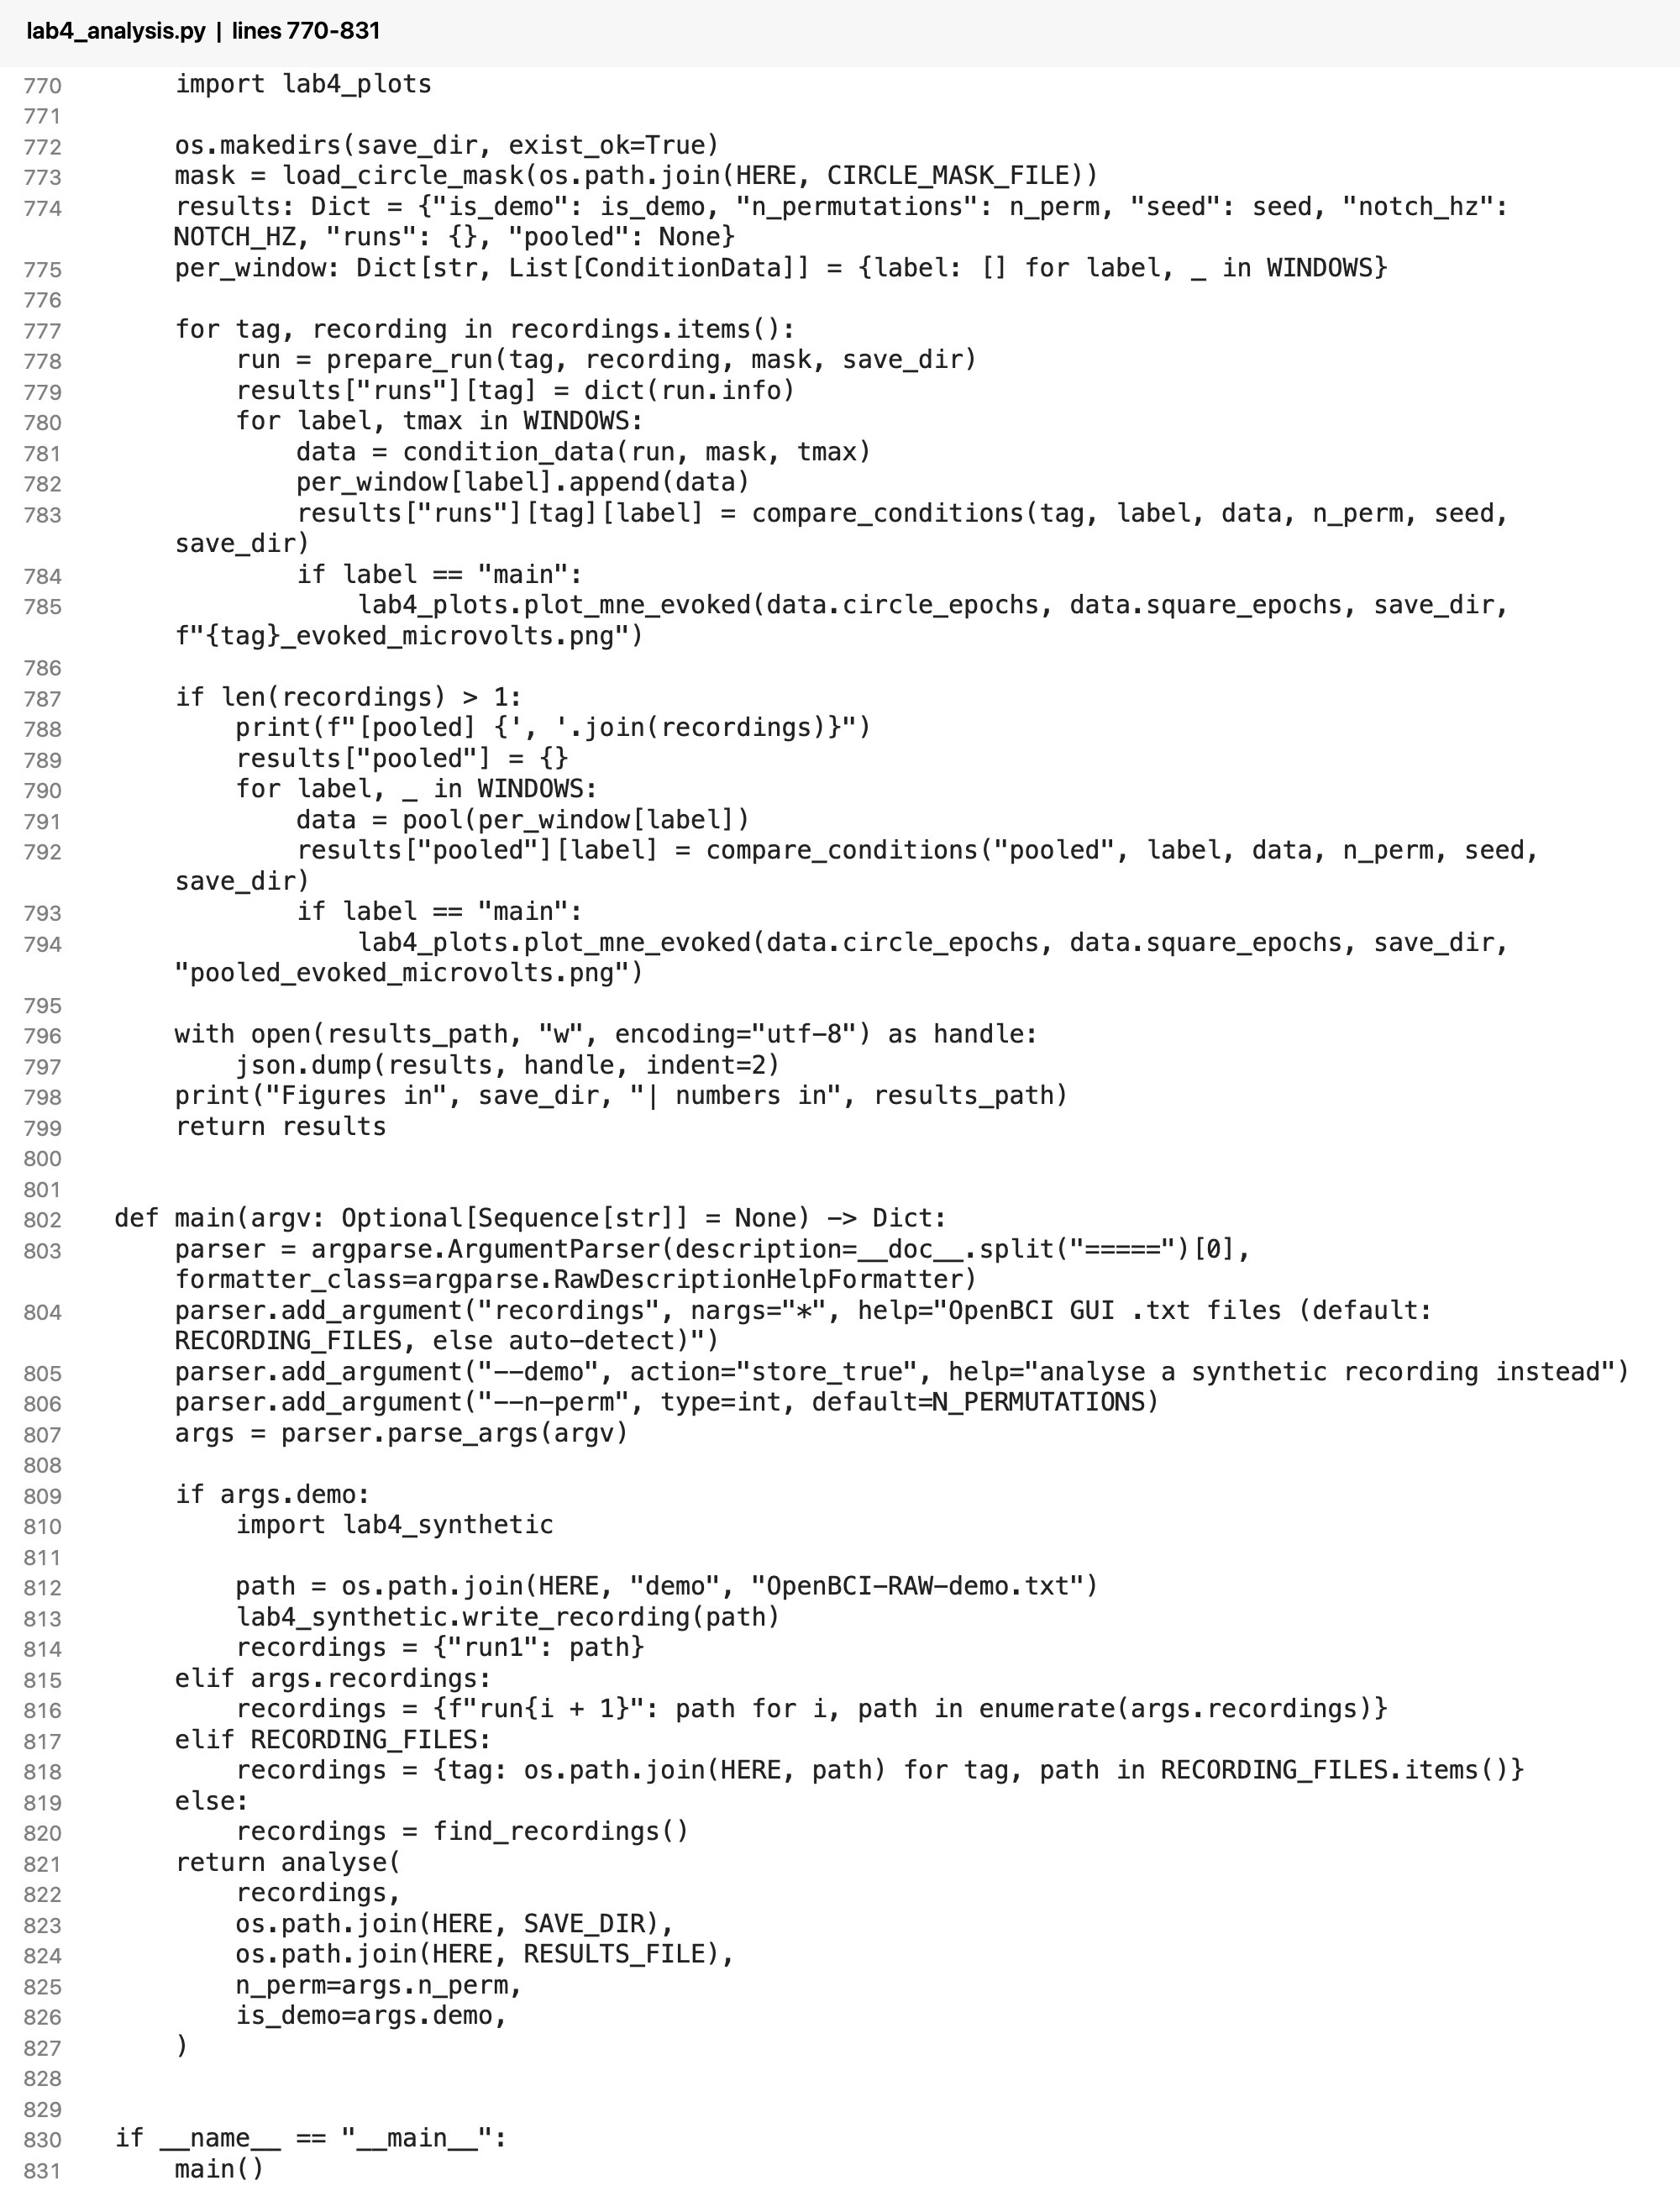
\includegraphics[width=\linewidth,height=0.92\textheight,keepaspectratio]{code_screenshots/analysis-12.png}
  \caption{\texttt{lab4\_analysis.py}, lines 770--831.}
\end{figure}


\end{document}
